% !TEX Program = lualatex
% class
\documentclass[ngerman]{scrartcl}

% input preamble
\usepackage{iftex}

% text input and font
\ifluatex  % LuaLaTeX
    \usepackage{fontspec}
    % main font automatically: Latin Modern
    \IfFontExistsTF{Fira Code}{% true branch
        \setmonofont{Fira Code}[
            Contextuals=Alternate,  % Activate the calt feature
            StylisticSet={1,3,5,8}, % fontspec docs S. 46
            CharacterVariant={16}, % fontspec docs S. 37
            Numbers={SlashedZero} % fontspec docs S. 44
        ]}{% false branch
    }
\else  % pdfLaTeX
    \usepackage[utf8]{inputenc}  % input in UTF-8
    \usepackage[T1]{fontenc}  % output in T1 fonts (west European encoding)
    \usepackage{lmodern}  % Latin modern font for main text
    \IfFileExists{fira.sty}{% true branch
        \usepackage[mono]{fira}  % Fira (not Code!) font for monospaced text
    }{% false branch
    }
\fi

% text processing
\usepackage{babel}  % language package
\usepackage[intlimits]{mathtools}  % upgrade of amsmath (automatically loaded) - \int^_ like \limits^_
\usepackage{amssymb}  % upgrade of amsfonts (American Math Society)
\usepackage{amstext}  % \text command in math environments
\usepackage{letltxmacro}  % \let command for robust macros (new sqrt)
\usepackage{chemformula}  % typeset chemical formulas


% page geometry
\usepackage{scrlayer-scrpage}  % page formatting with KOMA options
\usepackage[paper=a4paper, hmargin=3cm, vmargin=2.5cm, includehead, includefoot]{geometry}  % horizontal: 3cm, vertical: 2.5cm strict with or without headers and footers
\usepackage{tabto}  % tab stops
\NumTabs{8}  % 8 equally spaced of \textwidth tab stops



% floats
\usepackage[hypcap=false, labelfont=bf]{caption, subcaption}  % caption editing - hypcap warning with hyperref
% counter prefixed with section number and therefore reset at each section:
\counterwithin{figure}{section}
\counterwithin{table}{section}
\usepackage{float}  % for [H] (forced here) specifier
\usepackage{tabularray}  % better tables
\usepackage{caption}  % better captions


% graphical input
\usepackage{graphicx}  % input JPEG, PNG, PDF, etc.
\usepackage{pdfpages}  % input PDF as whole pages
\usepackage{lastpage}  % reference to last page
\usepackage{import} % include files from other directories


% text
\usepackage[locale=DE, uncertainty-mode=separate]{siunitx}  % SI units, German formatting - \pm stays \pm instead of ..(.)
\let\sqty\qty  % physics overrides \qty of siunitx, therefore make it available as \sqty
\usepackage{physics}  % macros for easier typesetting of physical formulas
\usepackage{icomma}  % no space after commas instead of English points) in decimal values
\usepackage{enumitem}  % better enumerating with style options
\usepackage{nicefrac}  % inline-fractions in n/d-style
\usepackage{xcolor}  % custom colors
%TU-Graz colors
\definecolor{TUred}{HTML}{e4154b}
\definecolor{TUgray}{HTML}{bcbcbc}
\usepackage{listings, scrhack}  % code display; listings in combination with KOMA
\ifluatex
    \IfFontExistsTF{Fira Code}{%
        \usepackage[verbatim]{lstfiracode}  % Fira Code in listings
        \lstset{style=FiraCodeStyle}
    }{}
\fi
\usepackage{fancyvrb}  % Verbatim environment with better options (capital V!)


% literacy
\usepackage[sorting=none, giveninits=true]{biblatex}  % defaults: backend=Biber, style=numeric
% bibliography styles: https://www.overleaf.com/learn/latex/Biblatex_bibliography_styles
% citation styles: https://www.overleaf.com/learn/latex/Biblatex_citation_styles
\usepackage{csquotes}  % better quotation - should also be used in combination with package babel (warning)
\usepackage{xurl}  % breaks links - after BibLaTeX, but before hyperref!
\usepackage[hidelinks]{hyperref}  % produces most errors, last to load


% enumerate paragraphs and subparagraphs
% depths: https://www.overleaf.com/learn/latex/Sections_and_chapters
% -1 \part{part}
%  0 \chapter{chapter}
%  1 \section{section}
%  2 \subsection{subsection}
%  3 \subsubsection{subsubsection}
%  4 \paragraph{paragraph}
%  5 \subparagraph{subparagraph}
\setcounter{secnumdepth}{3}


% KOMA setups
% header and footer
\pagestyle{scrheadings}  % KOMA style
\clearpairofpagestyles  % reset
\setkomafont{pageheadfoot}{\normalfont}  % standard font in header and footer
\setlength{\headheight}{27.2pt}  % warning
\cfoot{\pagemark{} / \pageref*{LastPage}}  % center foot - *: ref but no hyperlink
% {}: empty statement
% \ : protected space
% \,: small space
\DeclareTOCStyleEntry[linefill=\TOCLineLeaderFill]{tocline}{section}  % sections in TableOfContents with dotted lines
% source: https://tex.stackexchange.com/a/651532
\KOMAoptions{parskip=half-}  % paragraphs with half a line height space instead of indentation, last line with no special treatment


% package setups

% rewrite names (babel overwrites German with standard English names, therefore at document beginn [after everything is loaded])
\AtBeginDocument{\renewcommand{\refname}{Literaturverzeichnis}}
% others:
% \contentsname
% \listtablename
% \listfigurename

% make title in bibliography upright
\DeclareFieldFormat{title}{#1}  % https://tex.stackexchange.com/a/311837
% make size of url in bibliography smaller
\renewcommand{\UrlFont}{\footnotesize\ttfamily}  % https://tex.stackexchange.com/a/151115, https://www.overleaf.com/learn/latex/Font_sizes%2C_families%2C_and_styles


% xcolor
\definecolor{code_keyword}{HTML}{A06E9D}
\definecolor{code_string}{HTML}{AD6E3E}
\definecolor{code_comment}{HTML}{6A9955}
% \definecolor{keyword_pink}{HTML}{c678dd}
% \definecolor{vscode_bg}{HTML}{282c34}
% \definecolor{vscode_var}{HTML}{e06c75}
% \definecolor{vscode_comment}{HTML}{7f848e}
% \definecolor{vscode_constant}{HTML}{d19a66}
% \definecolor{vscode_function}{HTML}{61afe3}
% \definecolor{background_grey}{HTML}{f8f8f8}
% \definecolor{code_basic}{HTML}{D4D4D4}
% \definecolor{code_background}{HTML}{1E1E1E}

% custom siunitx units
\DeclareSIUnit{\dig}{dig}  % digits for uncertainty of electronical measurement devices
\DeclareSIUnit{\px}{px}  % pixels
\sisetup{table-align-uncertainty=true}


% listings
\lstset{
    basicstyle=\ttfamily\footnotesize,%\color{code_basic},  % \footnotesize contains \selectfont implicitly
    %backgroundcolor=\color{code_background},
    commentstyle=\color{code_comment},
    keywordstyle=\bfseries\color{code_keyword},
    numberstyle=\tiny,
    stringstyle=\color{code_string},
    breakatwhitespace=false,
    breaklines=true,
    captionpos=b,
    keepspaces=true,
    numbers=left,
    numbersep=5pt,
    showspaces=false,
    showstringspaces=false,
    showtabs=false,
    tabsize=2
}


% new sqrt
% https://en.wikibooks.org/wiki/LaTeX/Mathematics
\makeatletter
\let\oldr@@t\r@@t
\def\r@@t#1#2{%
    \setbox0=\hbox{$\oldr@@t#1{#2\,}$}\dimen0=\ht0
    \advance\dimen0-0.2\ht0
    \setbox2=\hbox{\vrule height\ht0 depth -\dimen0}%
    {\box0\lower0.4pt\box2}}
\LetLtxMacro{\oldsqrt}{\sqrt}
\renewcommand{\sqrt}[2][\ ]{\oldsqrt[#1]{#2} }
\makeatother


% own commands
% \newcommand* can't contain multiple lines
% \newcommand can
\newcommand*{\mup}[1]{\ensuremath{\text{\textup{#1}}}}  % math mode upright normal font
\newcommand*{\inkgraphics}[3][\linewidth]{\def\svgwidth{#1}\import{#2}{#3}}
\newcommand{\todo}[1]{\textbf{\textcolor{TUred}{#1\\}}}


% custom tabularray environments

% imports and setups of tabularray: {
%     expl3,
%     xparse,
%     ninecolors
%     \hypersetup{pdfborder={0 0 0}}
% }

% additionally loaded libraries:
% diagbox
% varwidth
% booktabs
% counter

\UseTblrLibrary{amsmath}  % +array, +matrix, +bmatrix, +Bmatrix, +pmatrix, +vmatrix, +Vmatrix and +cases like tabularray with graphical options
\UseTblrLibrary{siunitx}  % siunitx suited for tabularray
\UseTblrLibrary{diagbox}  % table cells with diagonal lines, suited for tabularray
\UseTblrLibrary{varwidth}  % measure cell width
\UseTblrLibrary{booktabs}
\UseTblrLibrary{counter}


% custom tabularray environments:

% info:
% colcycle: https://github.com/lvjr/tabularray/issues/74
% guard: https://github.com/lvjr/tabularray/issues/175#event-6567229210

% guard S columns if latest feature ={guard} is not yet available
\newcommand*{\SiGuard}[1]{{#1}}

% standard environment
\SetTblrInner{
    hlines,
    vlines,
    columns={
            halign=c,
            valign=m,
        },
    measure=vbox,
}

% X columns
\NewTblrEnviron{tblrx}
\SetTblrInner[tblrx]{
    hlines,
    vlines,
    columns={
            halign=c,
            valign=m,
            co=1,  % coefficient of width for expendable columns (X columns)
        },
    width=\linewidth,
    vspan=minimal,
    measure=vbox,
}

% -X columns
\NewTblrEnviron{tblr-x}
\SetTblrInner[tblr-x]{
    hlines,
    vlines,
    columns={
            halign=c,
            valign=m,
            co=-1,  % shrinks X column down to natural width
        },
    width=\linewidth,
    vspan=minimal,
    measure=vbox,
}

% no hline and vline left and on top of first cell
\NewTblrEnviron{tblr_omit_first_cell}
\SetTblrInner[tblr_omit_first_cell]{
    hlines,
    vlines,
    columns={
            halign=c,
            valign=m,
        },
    hspan=even,
    vspan=minimal,
    %
    hline{1}={1}{white},  % first row, only first cell
    vline{1}={1}{white},
    measure=vbox,
}

% longtblr
\DefTblrTemplate{conthead-text}{default}{(Fortsetzung)}  % default: define and set at the same time
\DefTblrTemplate{contfoot-text}{default}{Fortsetzung auf nächster Seite}
\SetTblrStyle{caption-tag}{font=\bfseries}  % caption tag bold
\SetTblrInner[longtblr]{
    hlines,
    vlines,
    columns={
            halign=c,
            valign=m,
        },
    measure=vbox,
}

% longtblr - to adjust width of caption 
\DefTblrTemplate{firsthead}{default}{\addtocounter{table}{-1}\captionof{table}[\InsertTblrText{entry}]{\InsertTblrText{caption}}}
\DefTblrTemplate{middlehead,lasthead}{default}{\addtocounter{table}{-1}\captionof{table}[]{\InsertTblrText{caption}~(Fortsetzung)}}
%info ADD this to a local environment around the longtblr: \captionsetup{format=plain,labelfont=bf,font=small,  width=\linewidth}
\usepackage{framed}

% manual header
\ihead{Interferometrie}  % inner (left) head
\chead{\textsc{Wachmann} Elias (12004232)\\\textsc{Zach} Andreas (12004790)}  % center head
\ohead{10.03.2023}  % outer (right) head

\addbibresource{Interferometrie.bib}



\begin{document}

%%%%Title Page %%%%
\begin{titlepage}
    \centering
    
\includegraphics[width=0.5\textwidth]{../../99_Misc/Logo_KF.pdf}\par\vspace{0.8cm}
    {\scshape\LARGE{Karl-Franzens-Universität Graz}\par}
    {\scshape\LARGE{Institut für Physik}\par}
    \vspace{1cm}
    {\scshape\Large{23S PHY.L02UB Fortgeschrittenenpraktikum 2}\par}
    678 Bachelorstudium Physik, UG2002/2021W\par
    \vspace{1.5cm}
    {\huge\bfseries II. Interferometrie\par}
    \vspace{2cm}
    \begin{table}[H]
        \centering
        \begin{tabular}{c c c}
            \Large Wachmann Elias &  & \Large Zach Andreas \\
            \Large 12004232       &  & \Large 12004790     \\
            \multicolumn{3}{c}{Gruppe 12}
        \end{tabular}
    \end{table}
    \vfill
    \Large Betreut von\par
    Thomas Georg \textsc{Boné}, BSc MSc
    \vfill
    % Bottom of the page
    {\large 10.03.2023\par}
\end{titlepage}
%%%%

\clearpage
\tableofcontents
\newpage

\section[Aufgabenstellung]{Aufgabenstellung \cite{ref:angabe}}
\label{sec:aufgabenstellung}

Der folgende Laborversuch besteht aus vier separaten Teilversuchen, welche sich abermals wie folgt in Unterversuche gliedern:

\begin{itemize}
    \item \textbf{Young'scher Doppelspalt}
          \begin{itemize}
              \item Aufzeichnen des Beugungsmusters von vier Doppelspalten mit unterschiedlichen Spaltbreiten und Spaltabständen % check
              \item Berechnen der Wellenlänge des Lasers % check
              \item Erklären der aufgezeichneten Beugungsmuster durch Vergleich mit theoretisch errechneten Mustern % TODO
              \item Aufzeichnen des Beugungsmusters eines Liniengitters % check
              \item Bestimmen der Gitterkonstante % check
          \end{itemize}
    \item \textbf{Wellenfront-Analyse / Shearing Interferometer}
          \begin{itemize}
              \item Vermessen des Interferenzmusters % check
              \item Berechnen des Wellenfrontradius % check
          \end{itemize}
    \item \textbf{Polarisation}
          \begin{itemize}
              \item Darstellen der winkelabhängigen Transmission zusammen mit dem theoretischen Verlauf % check
              \item Verifizieren des Gesetzes von Malus % TODO
              \item Untersuchen des Einflusses des Durchlasswinkels eines weiteren Polarisators zwischen zwei gekreuzten Polarisatoren % TODO
          \end{itemize}
    \item \textbf{Michelson Interferometer}
          \begin{itemize}
              \item Justieren und generieren von konzentrischen Interferenzmustern % check
              \item Bestimmen der Wellenlänge des Lasers durch Weglängenänderung % check
              \item Untersuchen des absoluten Weglängenunterschieds in den beiden Interferometerarmen sowie Auflösung und Stabilität des Interferometers % TODO
              \item Justieren und generieren von streifenförmigen Interferenzmustern % check
              \item Untersuchen der Rolle der Polarisation auf die Interfenzfähigkeit des Laserlichts % TODO
          \end{itemize}
\end{itemize}


\section[Grundlagen]{Grundlagen \cite{ref:angabe}}
\label{sec:grundlagen}

\subsection{Young'scher Doppelspalt}
\label{sec:grundlagen_youngscher_doppelspalt}

Bescheint man mit einer Lichtquelle zwei eng beieinanderliegende Spalte mit dem Abstand $d$ und projiziert das Bild auf einen ansonsten undurchsichtigen Schirm, so wirkt der Spalt als kohärente Lichtquelle. Dies ist evident für eine kohärente Lichtquelle, gilt für eine thermische Lichtquelle aber nur unter der Bedingung räumlicher Kohärenz. Die Wellen aus den Spalten überlagern sich in Abhängigkeit vom Beobachtungswinkel konstruktiv oder destruktiv, was auf einen Schirm projiziert eine Abfolge an Intensitätsmaxima und -minima ergibt.

Konstruktive Interferenz tritt bei ganzzahlig Vielfachen $n$ der Wellenlänge $\lambda$ auf, dies nennt man auch den \textit{optischen Gangunterschied} $\Delta$.
\begin{equation}
    \label{eq:konstruktive_interferenz}
    \Delta = n \lambda
\end{equation}
Unter der Bedingung, dass der Abstand zwischen Doppelspalt und Beobachtungsebene $z$ viel größer als der Spaltabstand $d$ ist, ergibt sich der optische Gangunterschied in die durch den Winkel $\phi$ definierte Richtung als
\begin{equation}
    \label{eq:optischer_gangunterschied}
    \Delta = \frac{2 \pi d}{\lambda} \sin(\phi)
\end{equation}
mit $\lambda$ der Wellenlänge.
Mit der Näherung $\sin(\phi) \approx \nicefrac{x}{z}$ (erfüllt für große Abstände $z$ zwischen Doppelspalt und Schirm, $x$ Abstand vom 0. Maximum zum n. Maximum) ergibt sich ein Streifenmuster mit der Periode $x$ der Form
\begin{equation}
    \label{eq:intensity_interferenz}
    I_{\text{Interferenz}}(x) = I_0 \left(1 + \cos(\frac{2 \pi x d}{\lambda z}) \right)
\end{equation}
Dafür wurde die endliche Breite des Spalts vernachlässigt bzw. ein unendlich schmaler Spalt angenommen. Tatsächlich überlagert sich dem Interferenzmuster das Beugungsmuster des Einzelspalts, das i.A. symmetrisch mit zu größeren Winkeln hin abnehmender Intensität ist. Ein einzelner rechteckiger Spalt der Breite $D$ führt zu einem Beugungsmuster der Form
\begin{equation}
    \label{eq:intensity_beugung}
    I_{\text{Beugung}}(x) = I_0 \cdot \frac{\sin^2(\frac{\pi D x}{\lambda z})}{\left(\frac{\pi D x}{\lambda z}\right)^2}
\end{equation}
Das Beugungsmuster des Doppelspalts ergibt sich multiplikativ als
\begin{equation}
    \label{eq:intensity_gesamt}
    I(x) = I_{\text{Interferenz}}(x) \cdot I_{\text{Beugung}}(x).
\end{equation}
Möchte man abschließend noch den optischen Gangunterschied mit den Abständen vom und auf dem Schirm in Verbindung bringen, so ergibt sich \autoref{eq:konstruktive_interferenz_approx}.
\begin{equation}
    \label{eq:konstruktive_interferenz_approx}
    n \lambda = d \cdot \frac{x}{z}
\end{equation}

Ein Liniengitter ist de facto nur eine Ansammlung vieler Spalte, gewissermaßen ein $N$-fachspalt. Allgemein treten bei einem Gitter Beugungs- und Interferenzeffekt auf (wie bei \autoref{eq:intensity_gesamt}), dies beschreibt \autoref{eq:intensity_gitter}. $N$ beschreibt dabei die Anzahl an Spalten, die mit der Intensität $I_0$
bestrahlt werden, $D$ die Breite des Spaltes, $d$ den Abstand zwischen den benachbarten Spalten, $\lambda$ die Wellenlänge des Lichtes und $\theta$ den Winkel zur Flächennormale.
\begin{equation}
    \label{eq:intensity_gitter}
    I(\theta) = I_0 \cdot \underbrace{\left[ \frac{\sin(N \pi \cdot \nicefrac{d}{\lambda} \cdot \sin(\theta))}{\sin(\pi \cdot \nicefrac{d}{\lambda} \cdot \sin(\theta))} \right]^2}_{\text{Gitterfunktion}} \cdot \underbrace{\left[ \frac{\sin(\pi \cdot \nicefrac{D}{\lambda} \cdot \sin(\theta))}{(\pi \cdot \nicefrac{D}{\lambda} \cdot \sin(\theta))} \right]^2}_{\text{Einzelspaltfunktion}}
\end{equation}
Möchte man abschließend noch den optischen Gangunterschied mit den Abständen vom und auf dem Schirm in Verbindung bringen, so ergibt sich \autoref{eq:konstruktive_interferenz_approx}.
\begin{equation}
    \label{eq:konstruktive_interferenz_approx_gitter}
    n \lambda = g \cdot \frac{x}{z}
\end{equation}
wobei $g$ die Gitterkonstante bezeichnet.


\subsection{Shearing-Interferometer / Wellenfront-Analyse}
\label{sec:grundlagen_shearing_interferometer}

Das Erscheinungsbild von optischen Interferenzmustern ist sowohl durch die Natur der Lichtwelle als auch der optischen Grenzflächen bestimmt, man denke an die färbigen Interferenzen auf Seifenblasen. Entsprechend ist es möglich, aus der Beobachtung von Interferenzen an Grenzflächen bekannter Geometrie auf die Eigenschaften der Lichtwelle zu schließen.
%? Evtl. Bilder
Beim Shearing-Interferometer handelt es sich um ein simples Interferometer, mit dem bestimmt werden kann, ob ein Lichtstrahl kollimiert, konvergent oder divergent ist. Dazu trifft das Licht unter \SI{45}{\degree} auf eine Glasplatte (in Seitenansicht, siehe \autoref{fig:shearing_interferometer}a), welche keilförmig ausgeführt ist. Durch die Reflexion an der vorderen und hinteren Fläche der Glasplatte entstehen zwei reflektierte Strahlen (\autoref{fig:shearing_interferometer}a), in deren Überlappungsbereich Interferenz auftritt (\autoref{fig:shearing_interferometer}b). Durch die keilförmige Geometrie führt dies für einen kollimierten Strahl zu einem zur Einfallsebene des Lichts parallelen Streifenmuster (\autoref{fig:shearing_interferometer}b). Ein konvergierender bzw. divergierender Strahl führt dagegen nach \autoref{fig:shearing_interferometer}b zu einem gedrehten Streifenmuster. Aus dem lateralen Versatz der beiden reflektierten Strahlen $l$, dem Streifenabstand $s$ und dem (auf die Senkrechte bezogenen) Winkel der Interferenzstreifen $\Theta$ (siehe \autoref{fig:shearing_interferometer}b) lässt sich der Radius $r$ der Wellenfront mit
\begin{equation}
    \label{eq:radius_wellenfront}
    r = \frac{ls}{\lambda \cdot \sin(\Theta)}
\end{equation}
berechnen.

\begin{figure}[H]
    \centering
    \begin{samepage}
        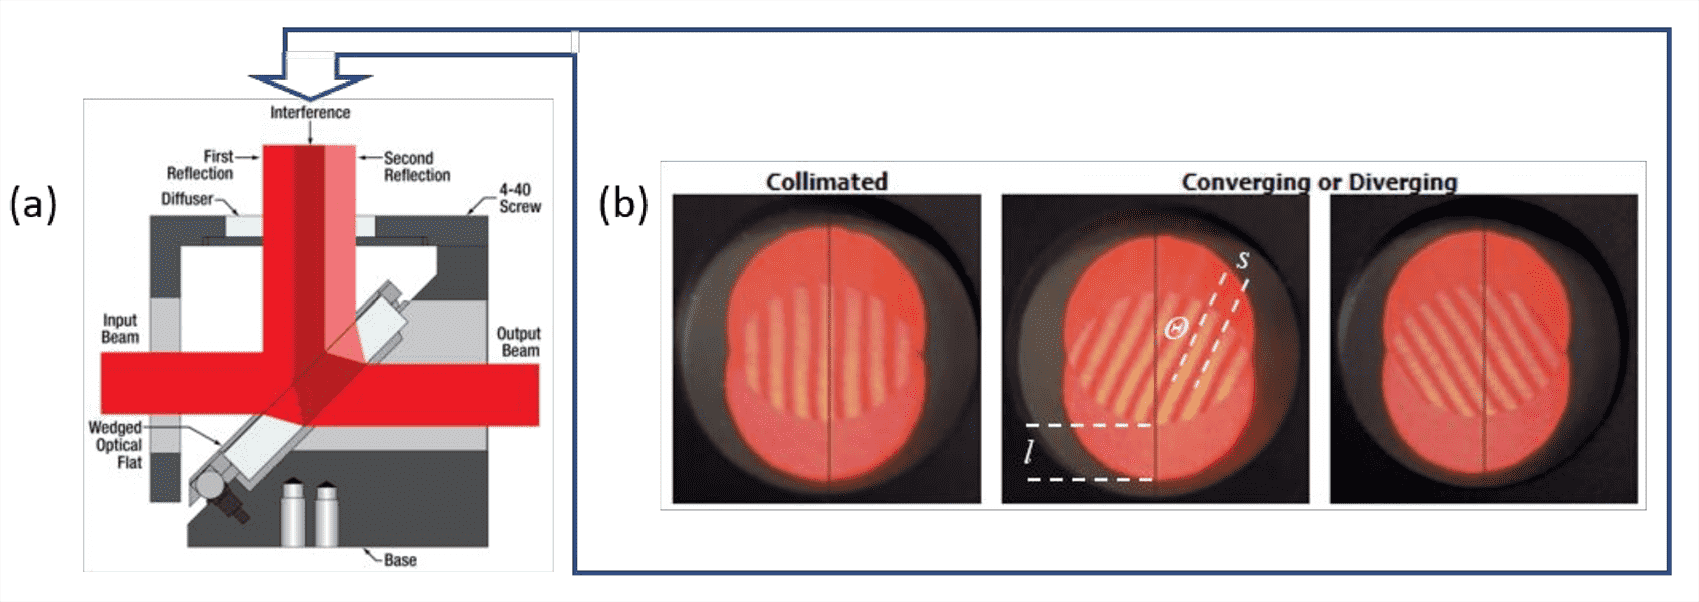
\includegraphics[width=0.8\linewidth]{fig/Compressed/Angabe_Abb5.png}
        \caption[Shearing-Interferometer]{Shearing-Interferometer. (a) Schematischer Aufbau in Seitenansicht, (b) beobachtete
            Interferenzmuster (in Aufsicht) für kollimierte, konvergierende und divergierende Wellenfronten, im
            mittleren Bild sind die im Text besprochenen Bestimmungsgrößen eingezeichnet. \copyright{} Thorlabs, Quelle: \cite{ref:angabe}}
        \label{fig:shearing_interferometer}
    \end{samepage}
\end{figure}


\subsection{Polarisation}
\label{sec:grundlagen_polarisation}

Für den Fall linearer Polarisation gilt für die transmittierte Intensität durch einen Polarisator mit der Durchlassrichtung entlang der durch den Winkel Null definierten Richtung das Gesetz von Malus.
\begin{equation}
    I(\alpha) = I_0 \cos^2(\alpha)
\end{equation}
Die nicht transmittierte Intensität wird je nach Art des Polarisators absorbiert oder reflektiert. Die Polarisation ist entscheidend für die Interferenzfähigkeit von Licht, es gelten die vier Gesetze nach Fresnel und Arago.
%? Is diese Anmerkung nötig?
%? \textbf{(siehe dazu auch einen entsprechenden Versuch mit dem Michelson-Interferometer)}.
\begin{framed}
    \begin{itemize}
        \item In dieselbe Richtung linear polarisierte Lichtstrahlen interferieren (wie nicht polarisiertes Licht).
        \item Zueinander senkrecht linear polarisierte Lichtstrahlen interferieren nicht (mit den nachfolgend aufgelisteten zwei Einschränkungen).
        \item Zueinander senkrecht linear polarisierte Lichtstrahlen interferieren, wenn sie ursprünglich dieselbe Polarisationsebene besaßen und wieder in diese zurückgeführt werden.
        \item  Zueinander senkrecht linear polarisierte Lichtstrahlen interferieren nicht, wenn sie in dieselbe Polarisationsebene zurückgeführt werden, diese aber nicht ursprünglich besaßen.
    \end{itemize}
\end{framed}

\subsection{Michelson-Interferometer}
\label{sec:grundlagen_michelson_interferometer}

Der prinzipielle Strahlengang eines Michelson-Interferometers ist in \autoref{fig:michalson_interferometer} dargestellt. Ein Lichtstrahl aus einer (Laser-)Quelle (1) wird an einem Strahlteiler (2) aufgeteilt. Der Strahlteiler ist ein dünnes Glasplättchen mit einer teilreflektierenden Schicht auf einer Fläche. Die beiden resultierenden Lichtstrahlen werden an zwei Spiegeln reflektiert und am Strahlteiler wieder vereint. Die Lichtstrahlen im Detektorarm treffen auf den Schirm (4), wo sie sich in Abhängigkeit vom Unterschied der Weglängen $s_1$ und $s_2$ überlagern. Für ebene Wellen der Form
\begin{equation}
    E(x,t) = E_0 e^{\omega t - k x}
\end{equation}
ist die Lichtintensität am Beobachtungsschirm gegeben durch
\begin{equation}
    I = \nicefrac{1}{4} \cdot c \cdot \varepsilon_0 \cdot E_0^2 \cdot (1 + \cos(\Delta \varphi))
\end{equation}
wobei $\Delta \phi$ die Phasendifferenz bezeichnet, die mit dem Unterschied der Weglängen\linebreak
$\Delta s = \left| s_1 - s_2 \right|$ nach $\Delta \varphi = (\nicefrac{2 \pi}{\lambda})\Delta s$ zusammenhängt.

\begin{figure}[H]
    \centering
    \begin{samepage}
        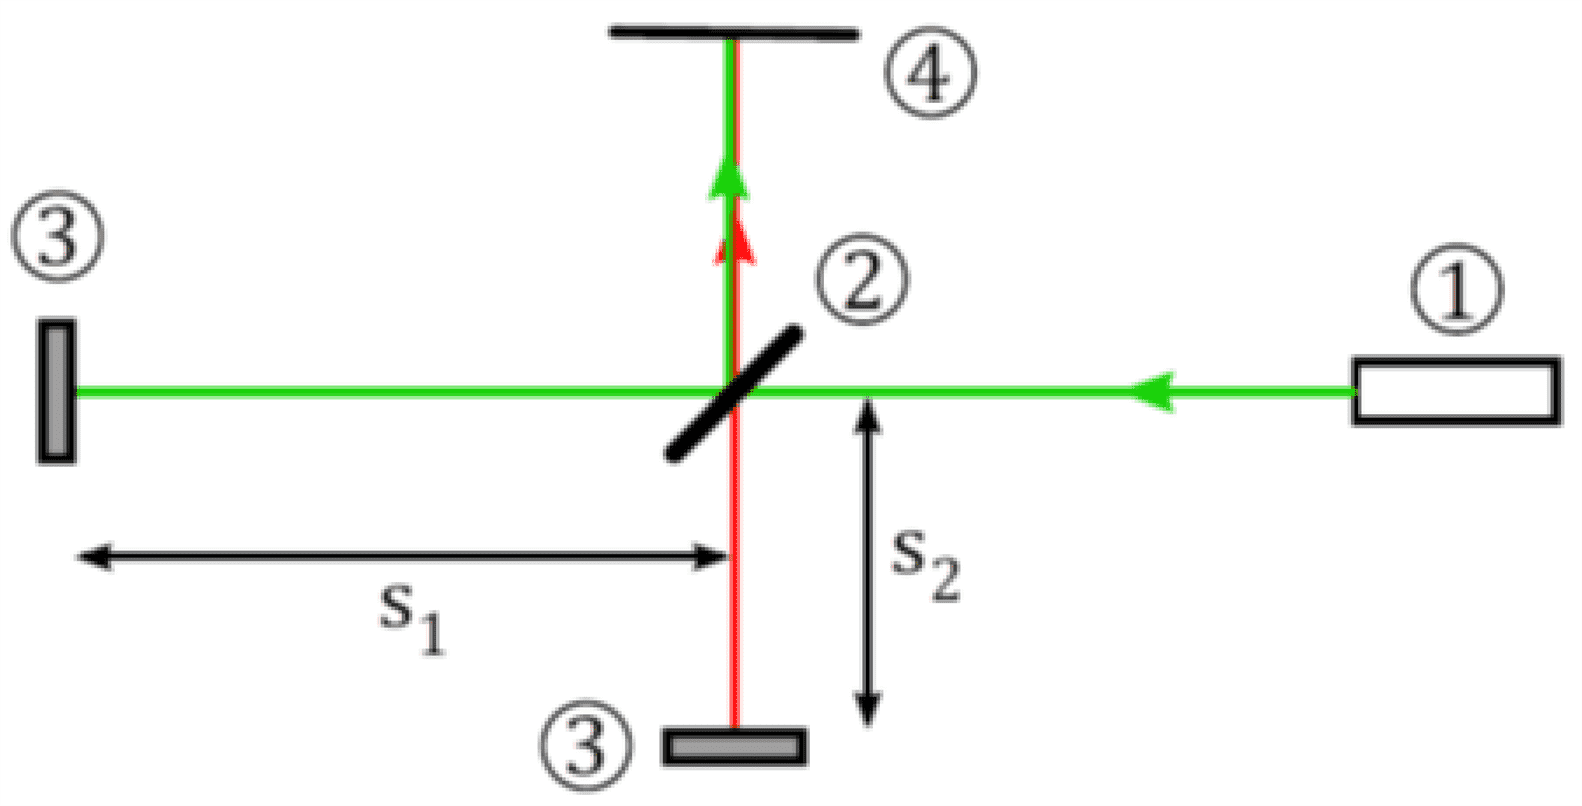
\includegraphics[width=0.6\linewidth]{fig/Compressed/Angabe_Abb8.png}
        \caption[Michelson-Interferometer]{Michelson-Interferometer. Strahlengang im Michelson-Interferometer. Ein Laserstrahl aus der Quelle (1) wird am Strahlteiler (2) aufgeteilt, die beiden Teilstrahlen durchlaufen die beiden Interferometerarme der Länge s1 und s2. Nach ihrer Reflexion an den Spiegeln (3,4) werden die Teilstrahlen am Strahlteiler wieder überlagert und interferieren am Beobachtungsschirm (4). \copyright{} Thorlabs, Quelle: \cite{ref:angabe}}
        \label{fig:michalson_interferometer}
    \end{samepage}
\end{figure}

Es stellt sich die Frage, wo bei destruktiver Interferenz im Detektorarm die Energie der Lichtwellen bleibt. Tatsächlich hat das Interferometer ja zwei \enquote{Ausgänge}, wobei einer eben zum Beobachtungsschirm, der zweite zurück zum Laser führt. Tatsächlich beobachtet man in zweiterem konstruktive Interferenz, wenn am Schirm destruktive Interferenz (also keine Lichtintensität) zu beobachten ist.

Das am Schirm beobachtete Interferenzmuster reagiert empfindlich auf kleine Änderungen in der Richtung des einfallenden Laserstrahls und in der Ausrichtung der Spiegel. Gleichzeitig sind diese Änderungen durch den nur wenige Millimeter durchmessenden Strahl schwer zu beobachten. Deshalb wird der Strahl durch eine Linse aufgeweitet, was zwischen Laser und Strahlteiler oder zwischen Strahlteiler und Schirm geschehen kann. Ersteres führt zu einem konzentrischen Interferenzmuster, zweiteres zu parallelen Interferenzstreifen. Wie in \autoref{fig:interferenzmuster_michelson_interferometer}a skizziert, können divergierende Strahlen auf (bei Vorliegen eines Weglängenunterschieds $\Delta s$ zwischen den beiden Interferometerarmen) auf zwei virtuelle Lichtquellen A und B zurückgeführt werden, wodurch sich das Auftreten eines konzentrischen Interferenzmusters erklärt. Gleichzeitig kann dieses genutzt werden, um die Interferometerarme auf die gleiche Länge einzustellen (im Prinzip auf einen Bruchteil der Wellenlänge), da sich dabei nach \autoref{fig:interferenzmuster_michelson_interferometer}b die Größe des zentralen Interferenzspots maximiert.

Ändert man den Weglängenunterschied der Interferometerarme, so ändern sich auch das Interferenzmuster und wandern nach innen bzw. außen (für die Interferenzringe, je nach Richtungsänderung) bzw. nach links oder rechts (für die Interferenzstreifen, wieder je nach Richtungsänderung), wo sie dann letztlich \enquote{verschwinden}. Die Anzahl an generierten bzw. vernichteten (gekrümmten oder geraden) Interferenzstreifen bei einem bestimmten Weglängenunterschied ist indirekt proportional zur Wellenlänge $\lambda$ des Lasers nach \autoref{eq:wegunterschied_anzahl}:
\begin{equation}
    \label{eq:wegunterschied_anzahl}
    \Delta s = n \cdot \frac{\lambda}{2}
\end{equation}



\begin{figure}[H]
    \centering
    \begin{samepage}
        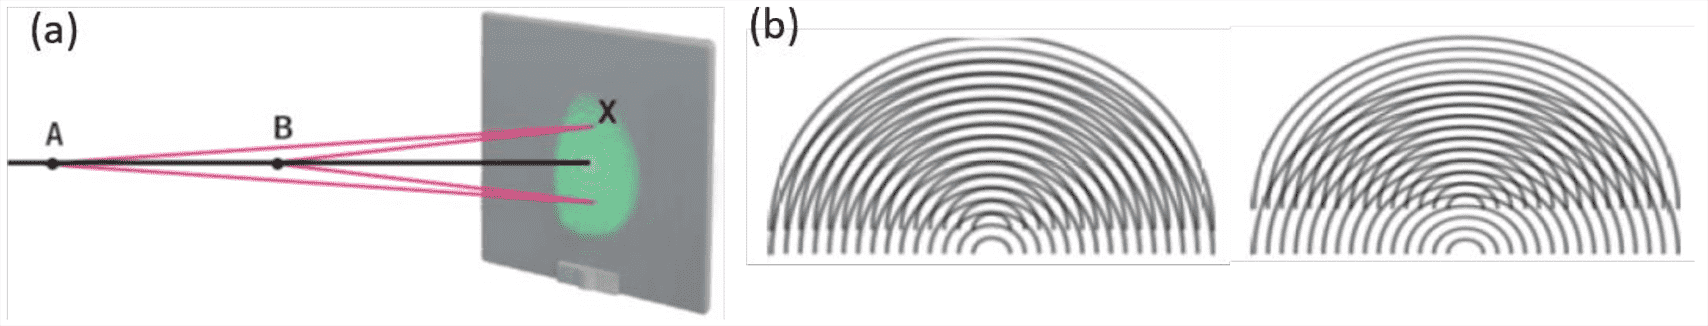
\includegraphics[width=\linewidth]{fig/Compressed/Angabe_Abb9.png}
        \caption[Interferenzmuster Michelson-Interferometer]{Zum kreisförmigen Interferenzmuster beim Michelson-Interferometer. (a) Skizze zur Erklärung seiner Entstehung, (b) Skizze zur Erklärung der Größe des zentralen Maximums (oder Minimums). \copyright{} Thorlabs, Quelle: \cite{ref:angabe}}
        \label{fig:interferenzmuster_michelson_interferometer}
    \end{samepage}
\end{figure}

\subsection{Unsicherheitsanalyse}
\label{subsec:unsicherheitsanalyse}

Die Fehlerfortpflanzung der berechneten Werte basiert auf der Größtunsicherheitsmethode nach Gauß. Um diese Berechnungen zeiteffizient durchführen zu können, wird für jeden Unterpunkt der Laborübung ein Skript in \verb!Python! implementiert. Kernstück dessen ist das package \verb!uncertainties! \cite{ref:uncertainties}, das intern die Fehlerfortpflanzung berechnet. Gerundet wird nach den Angaben des Skriptums der Lehrveranstaltung \enquote{Einführung in die physikalischen Messmethoden} \cite{ref:messmethoden}.



\section{Geräteliste}
\label{sec:geraeteliste}

Für den praktischen Aufbau und die Messungen der geforderten Größen wurden die in \autoref{tab:geraeteliste} aufgelisteten Geräte und Hilfsmittel verwendet.

\begin{table}[H]
    \centering
    \begin{samepage}
        \caption[Geräteliste]{Verwendete Geräte und wichtige Materialien}
        \label{tab:geraeteliste}
        \begin{tblrx}{cells={font=\footnotesize}}
            Gerät                     & Hersteller              & Modell               & Messsbereich / Unsicherheit                                                           & Inventar-Nr. \\
            Laser                     & Thorlabs                & CPS532               & $\lambda = \SI{532}{nm}$                                                              & 22442-S01    \\
            diverse Spiegel           & Thorlabs                & KM100                & -                                                                                     & -            \\
            Graufilter                & Thorlabs                & NX1N/M               & -                                                                                     & -            \\
            Doppelspalte              & Phywe                   & 0852300              & -                                                                                     & -            \\
            Gitter                    & Phywe                   & 0852400              & -                                                                                     & -            \\
            Optischer Tisch           & -                       & -                    & -                                                                                     & -            \\
            diverse Halterungen       & Thorlabs                & -                    & -                                                                                     & -            \\
            Sammellinse               & Thorlabs                & FMP1/M               & $f = \SI{40}{mm}$                                                                     & -            \\
            Zerstreuungslinse         & Thorlabs                & FMP1/M               & $f = \SI{-16}{mm}$                                                                    & -            \\
            Shearing-Interferometer   & Thorlabs                & nicht vorhanden      & -                                                                                     & -            \\
            Lichtintensitätsmesser    & Sauter                  & SO 200k              & $\Delta I = (\pm \SI{3}{\percent}\text{rdg} \pm \SI{0.5}{\percent}\text{fs}) \cdot I$ & 51152203     \\
            Polarisationsfolie        & Nitto denko             & -                    & -                                                                                     & -            \\
            Maßband                   & Schuller Eh klar        & Power Tape \SI{3}{m} & Klasse II                                                                             & -            \\
            Michelson Interferometer  & -                       & -                    & -                                                                                     & -            \\
            Rohr                      & -                       & -                    & -                                                                                     & -            \\
            diverse Abbildungsschirme & Wand, Papier, Tür, etc. & -                    & -                                                                                     & -            \\
            Mobiltelefon              & OnePlus                 & 8 Pro                & -                                                                                     & -            \\
        \end{tblrx}
    \end{samepage}
\end{table}

Die verwendeten Doppelspalte haben die Abmessungen wie in \autoref{tab:doppelspalt_abmessungen} vermerkt.

\begin{table}[H]
    \centering
    \begin{samepage}
        \caption[Doppelspaltmaße]{Verwendete Doppelspalte mit der jeweiligen Nummer $i$, der Spaltbreite $D$ in \unit{\milli\meter} und dem Spaltabstand $d$ in \unit{\milli\meter}. Quelle: \cite{ref:angabe}}
        \label{tab:doppelspalt_abmessungen}
        \begin{tblr}{colspec={Q S[table-format=1.1]S[table-format=1.2]}, row{1}={guard}}
            $i$ / 1 & $D$ / \si{\milli\meter} & $d$ / \si{\milli\meter} \\
            1       & 0.2                     & 0.25                    \\
            2       & 0.1                     & 0.25                    \\
            3       & 0.1                     & 0.50                    \\
            4       & 0.1                     & 1.00                    \\
        \end{tblr}
    \end{samepage}
\end{table}

\paragraph{Anmerkung zu den Unsicherheiten:} Zur Unsicherheitsangabe werden die jeweiligen Unsicherheitsmaße der Geräte, welche aus den Datenblättern (sofern vorhanden) entnommen werden, verwendet. Für die analogen Messgeräte wird eine kombinierte Ablese- und Messunsicherheit von $\pm\SI{1}{Skalenstrich}$ verwendet.

Alle Teilversuche wurden bei einer Umgebungstemperatur von \SI{24(1)}{\celsius} einem Luftdruck von \SI{1000(10)}{\hecto\pascal} und einer relativen Luftfeuchtigkeit von \SI{33(1)}{\percent} durchgeführt.



\section{Versuchsaufbau}
\label{sec:aufbau}

\subsection{Young'scher Doppelspalt}
\label{sec:aufbau_doppelspalte}

Für den Aufbau zum Versuch \textit{Young'scher Doppelspalt} wird der Laser mittels zwei Spiegel auf das Plättchen mit den vier verschiedenen (siehe \autoref{tab:doppelspalt_abmessungen}) Doppelspalten gelenkt. Der Abstand vom Doppelspalt wird mit \SI{2520(5)}{\milli\meter} bestimmt -- wobei hier noch zur vom Maßband gegebenen Unsicherheit von \SI{1.1}{\milli\meter} eine weitere Unsicherheit durch das Messen in der Luft hinzukommt. Der Aufbau in \autoref{fig:aufbau_doppelspalt} zeigt den optischen Tisch, der Schirm ist rechts im oben angeführten Abstand an der Wand befestigt.
\begin{figure}[H]
    \centering
    \begin{samepage}
        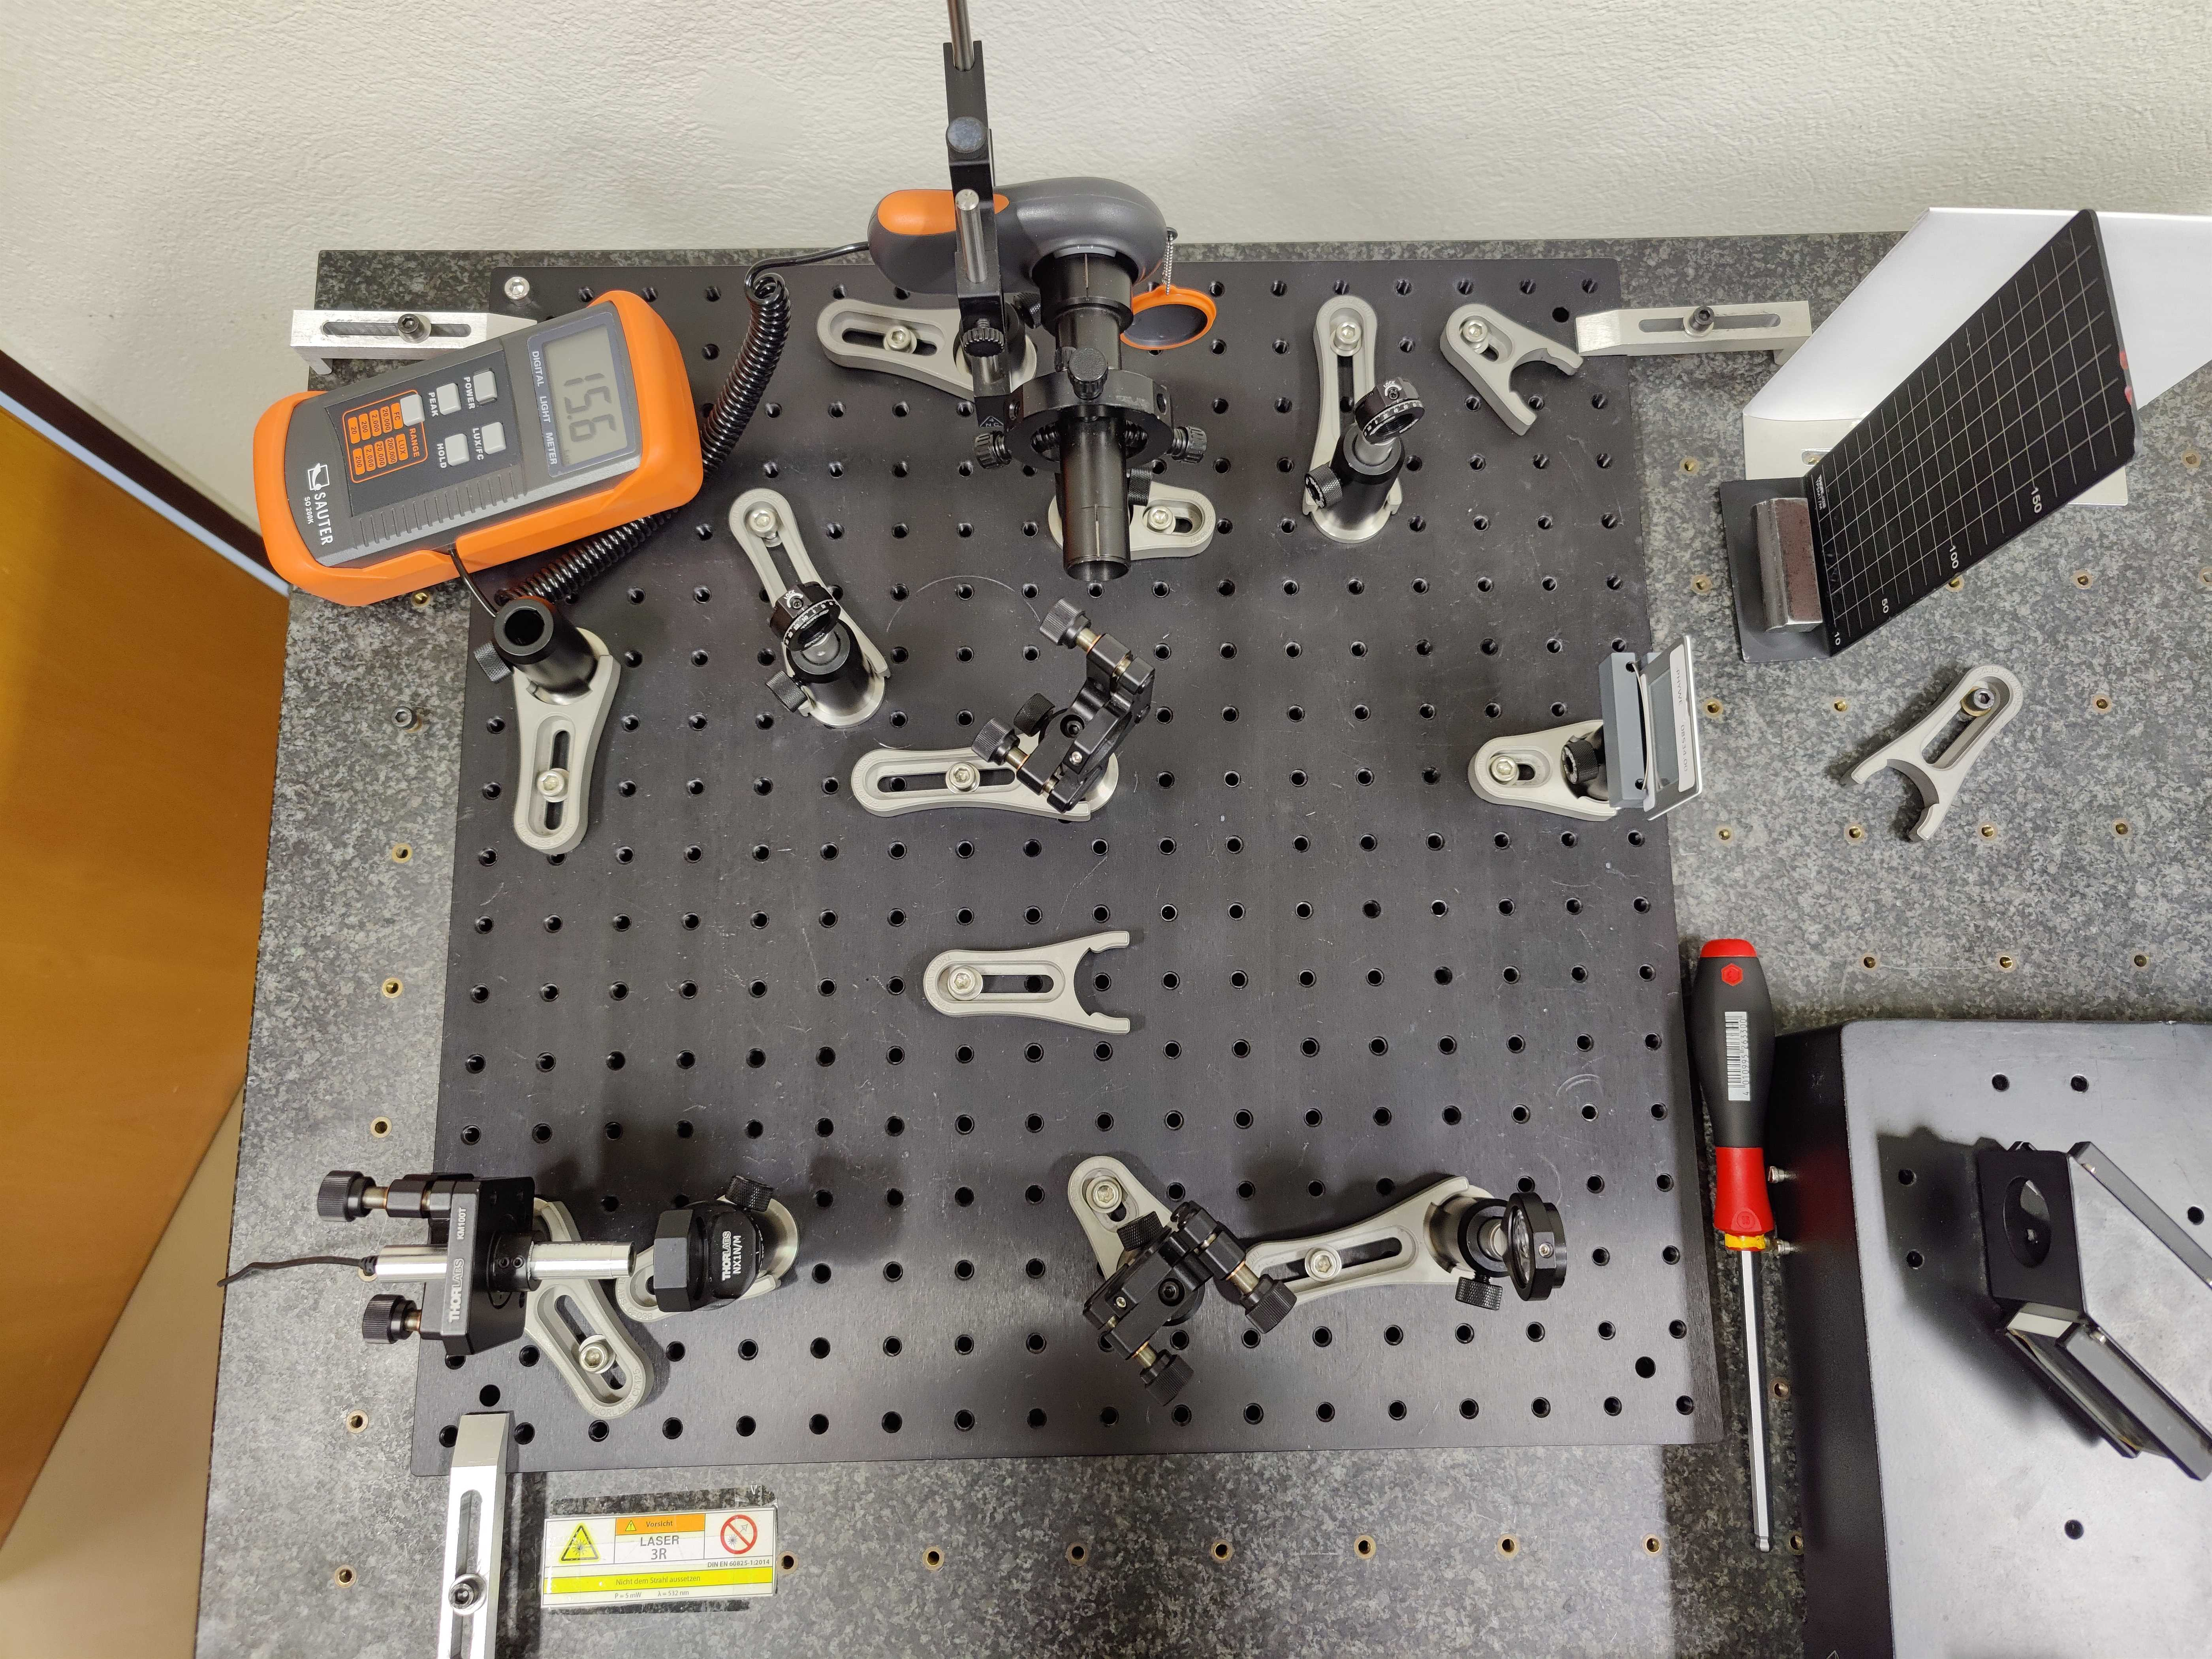
\includegraphics[width=0.7\linewidth]{fig/Compressed/aufbau_doppelspalt.jpg}
        \caption{Aufbau Young'scher Doppelspalt}
        \label{fig:aufbau_doppelspalt}
    \end{samepage}
\end{figure}


\subsection{Shearing-Interferometer}
\label{sec:aufbau_shearing}

Der Aufbau des Shearing-Interferometers ist in \autoref{fig:aufbau_shearing} gegeben. Dabei wird der untere Spiegel aus dem vorhergehenden Versuch wiederverwendet und der Laserstrahl auf die Frontalebene gelenkt, welche um \SI{45}{\degree} zur Tischebene geneigt ist.
%
\begin{figure}[H]
    \centering
    \begin{samepage}
        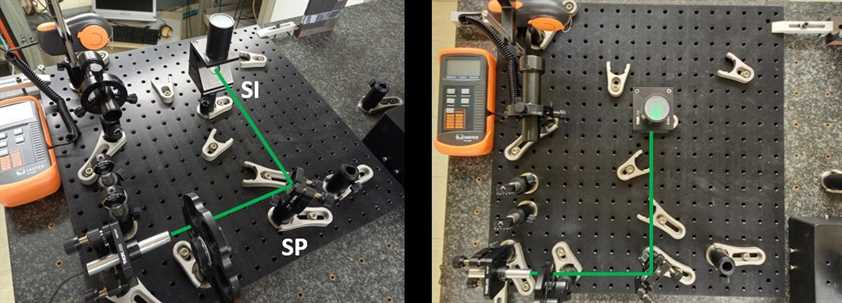
\includegraphics[width=0.9\linewidth]{fig/Compressed/shearing.jpg}
        \caption[Aufbau Shearing Interferometer]{Aufbau Shearing Interferometer. Quelle: \cite{ref:angabe}}
        \label{fig:aufbau_shearing}
    \end{samepage}
\end{figure}
%
\paragraph{Anmerkung zum Versuch:} Da sich das Shearing Interferometer leider zum Zeitpunkt der Übung in Reparatur befand, wird der Versuch im folgenden hyptotethisch abgehandelt.


\subsection{Polarisation}
\label{sec:aufbau_polarisation}

Anstelle des Shearing Interferometers werden jetzt zwei Polarisationsfilter in den Pfad des Lasers eingebracht. Nach dem zweitem Filter trifft der Laser auf einen Lichtintensitätsmesser, welcher wie in \autoref{fig:aufbau_polarisation} ersichtlich, durch ein Rohr von sonstigen Lichteinflüssen abgeschirmt wird.
%
\begin{figure}[H]
    \centering
    \begin{samepage}
        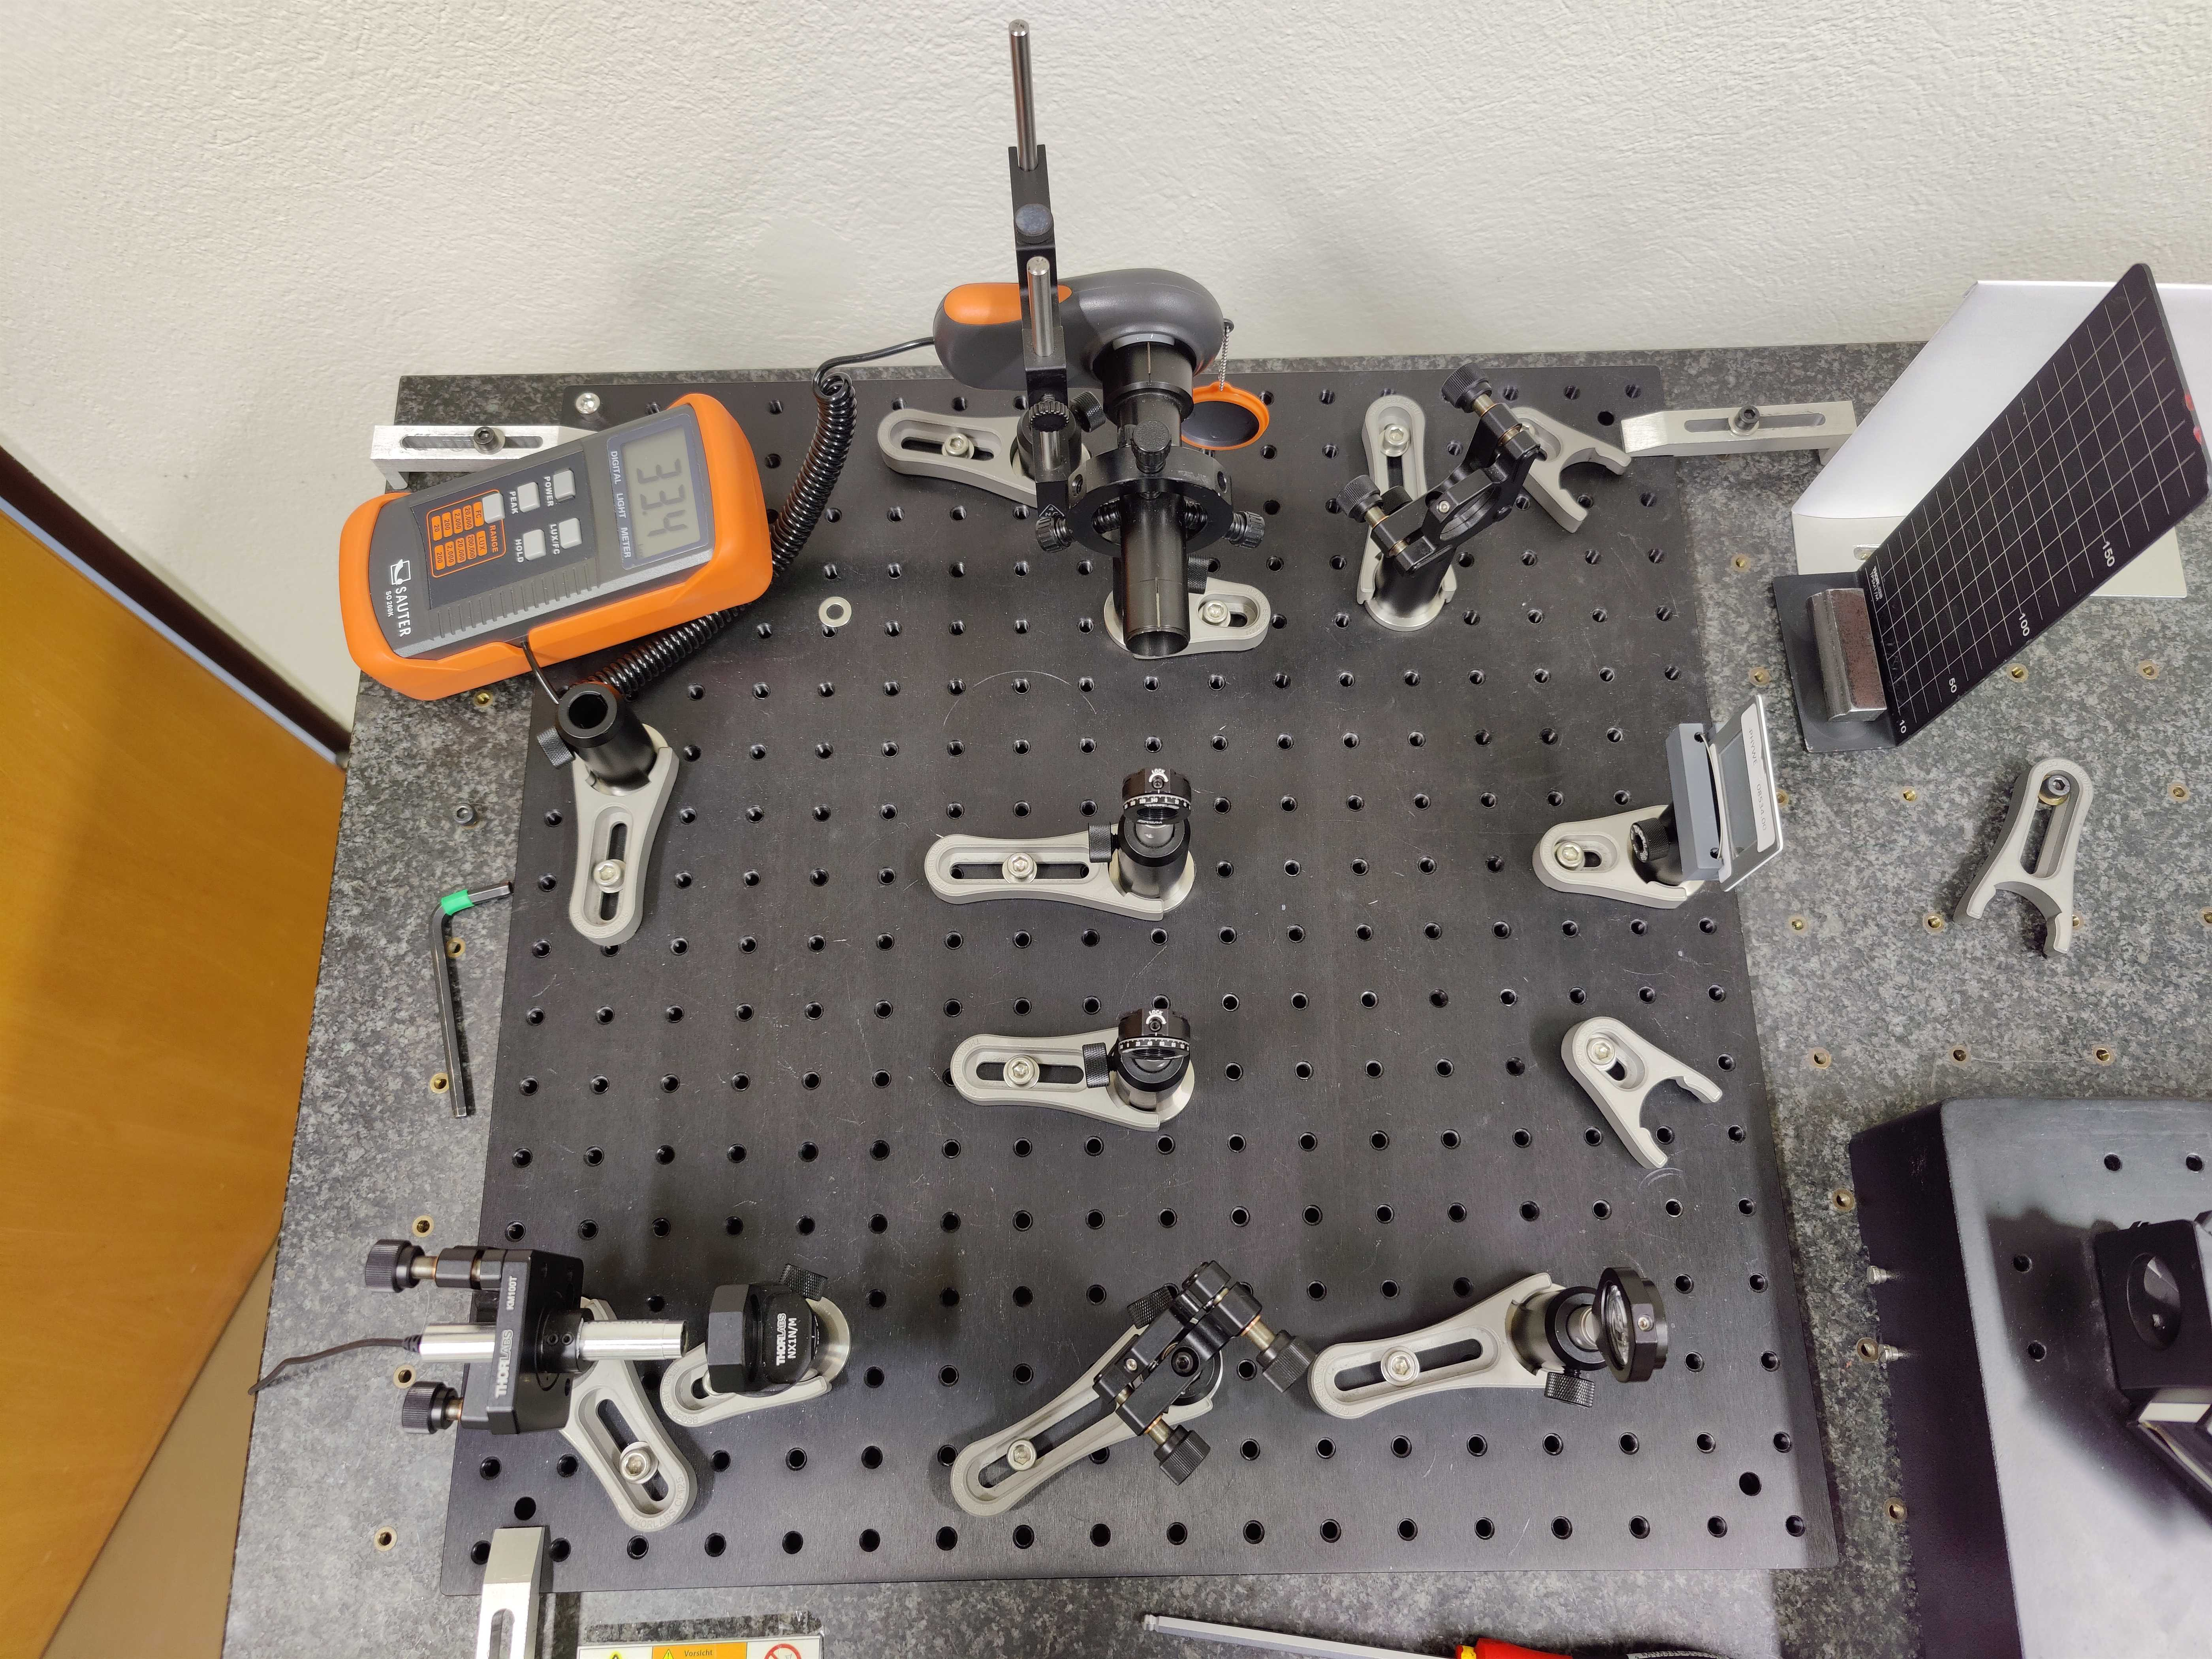
\includegraphics[width=0.7\linewidth]{fig/Compressed/Aufbau_polarisation.jpg}
        \caption{Aufbau Polarisation}
        \label{fig:aufbau_polarisation}
    \end{samepage}
\end{figure}


\subsection{Michelson-Interferometer}
\label{sec:aufbau_michelson}

Nun wird auch der letzte verbleibende Spiegel aus dem Strahlengang des Lasers gegeben und der Laserstrahl trifft so direkt auf das in \autoref{fig:aufbau_michelson} rechts gezeigte Michelson-Interferometer. Wie gut in der Abbildung ersichtlich ist, wird der Strahl im Michelson-Interferometer in die beiden Arme aufgeteilt. Nach letztlicher Zusammenführung der beiden Strahlen trifft der resultierende Strahl auf den Schirm.
Zur Untersuchung verschiedener Effekte wird je eine Sammel- bzw. Zerstreuungslinse in den Strahlengang zwischen Laser und Michelson-Interfereometer eingebracht.
%
\begin{figure}[H]
    \centering
    \begin{samepage}
        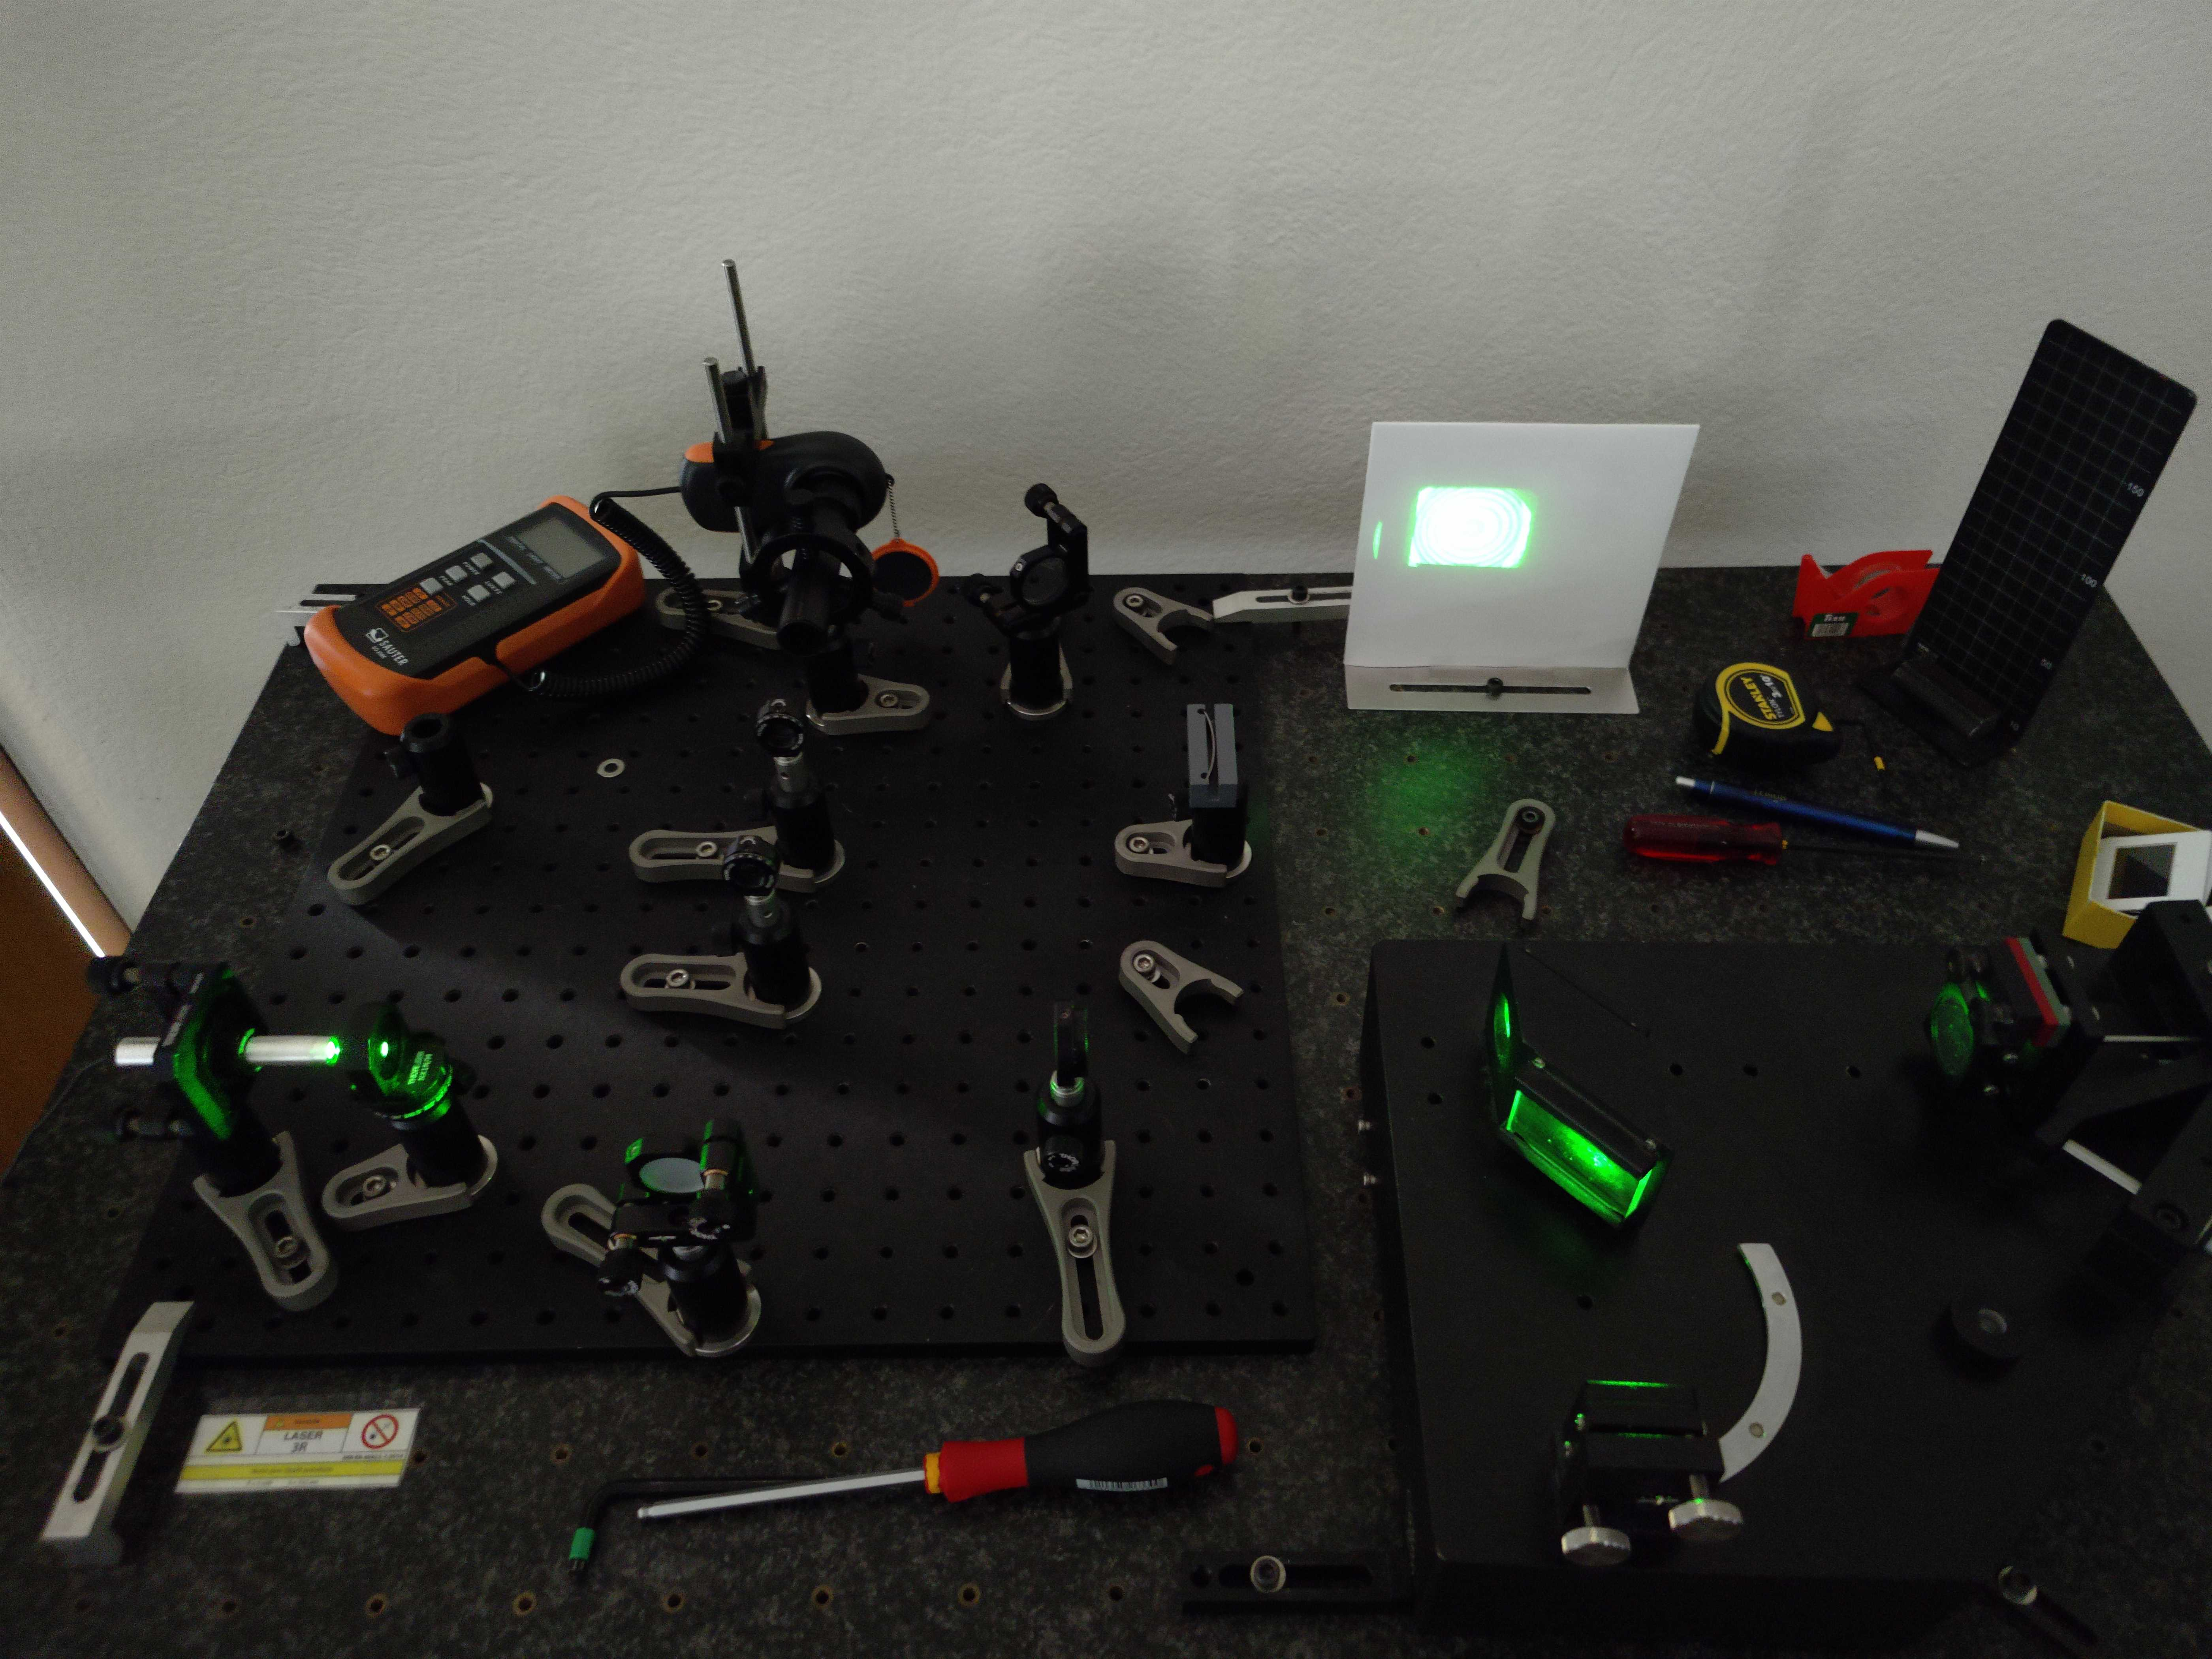
\includegraphics[width=0.7\linewidth]{fig/Compressed/aufbau_michelson.jpg}
        \caption{Aufbau Michelson-Interferometer}
        \label{fig:aufbau_michelson}
    \end{samepage}
\end{figure}



\section{Versuchsdurchführung}
\label{sec:durchfuehrung}

Vor jedem Teilversuch wird nochmals überprüft, ob sich der gewünschte optische Weg ergibt und der Laser nicht unkontrolliert oder ungewollt in nicht beabsichtige Richtungen abgelenkt wird. Weiters wird stets darauf geachtet, dass man nicht mit reflektierenden Gegenständen (z.B. Ring, Schraubenzieher) im Strahlengang hantiert.

\subsection{Young'scher Doppelspalt}
\label{sec:durchfuehrung_doppelspalt}

Der Versuch wird gemäß der Beschreibung in \autoref{sec:aufbau_doppelspalte} aufgebaut und die in \autoref{tab:doppelspalt_abmessungen} angeführten Doppelspalte werden der Reihe nach vom Laser durchstrahlt. Der $l_\text{Schirm} = \SI{2520(5)}{\milli\meter}$ entfernte Schirm -- ein karriertes A4-Blatt an der Wand -- wird nun vom sich ergebenden Interferenzmuster beleuchtet.

Es ergeben sich für die vier Doppelspalte folgende Interferenzbilder in den Abbildungen \ref{fig:DS_1_interferenzmuster} bis \ref{fig:DS_2_interferenzmuster}.
%
\setcapindent{0pt}
\begin{figure}[H]
    \centering
    \begin{minipage}[t]{0.45\linewidth}
        \centering
        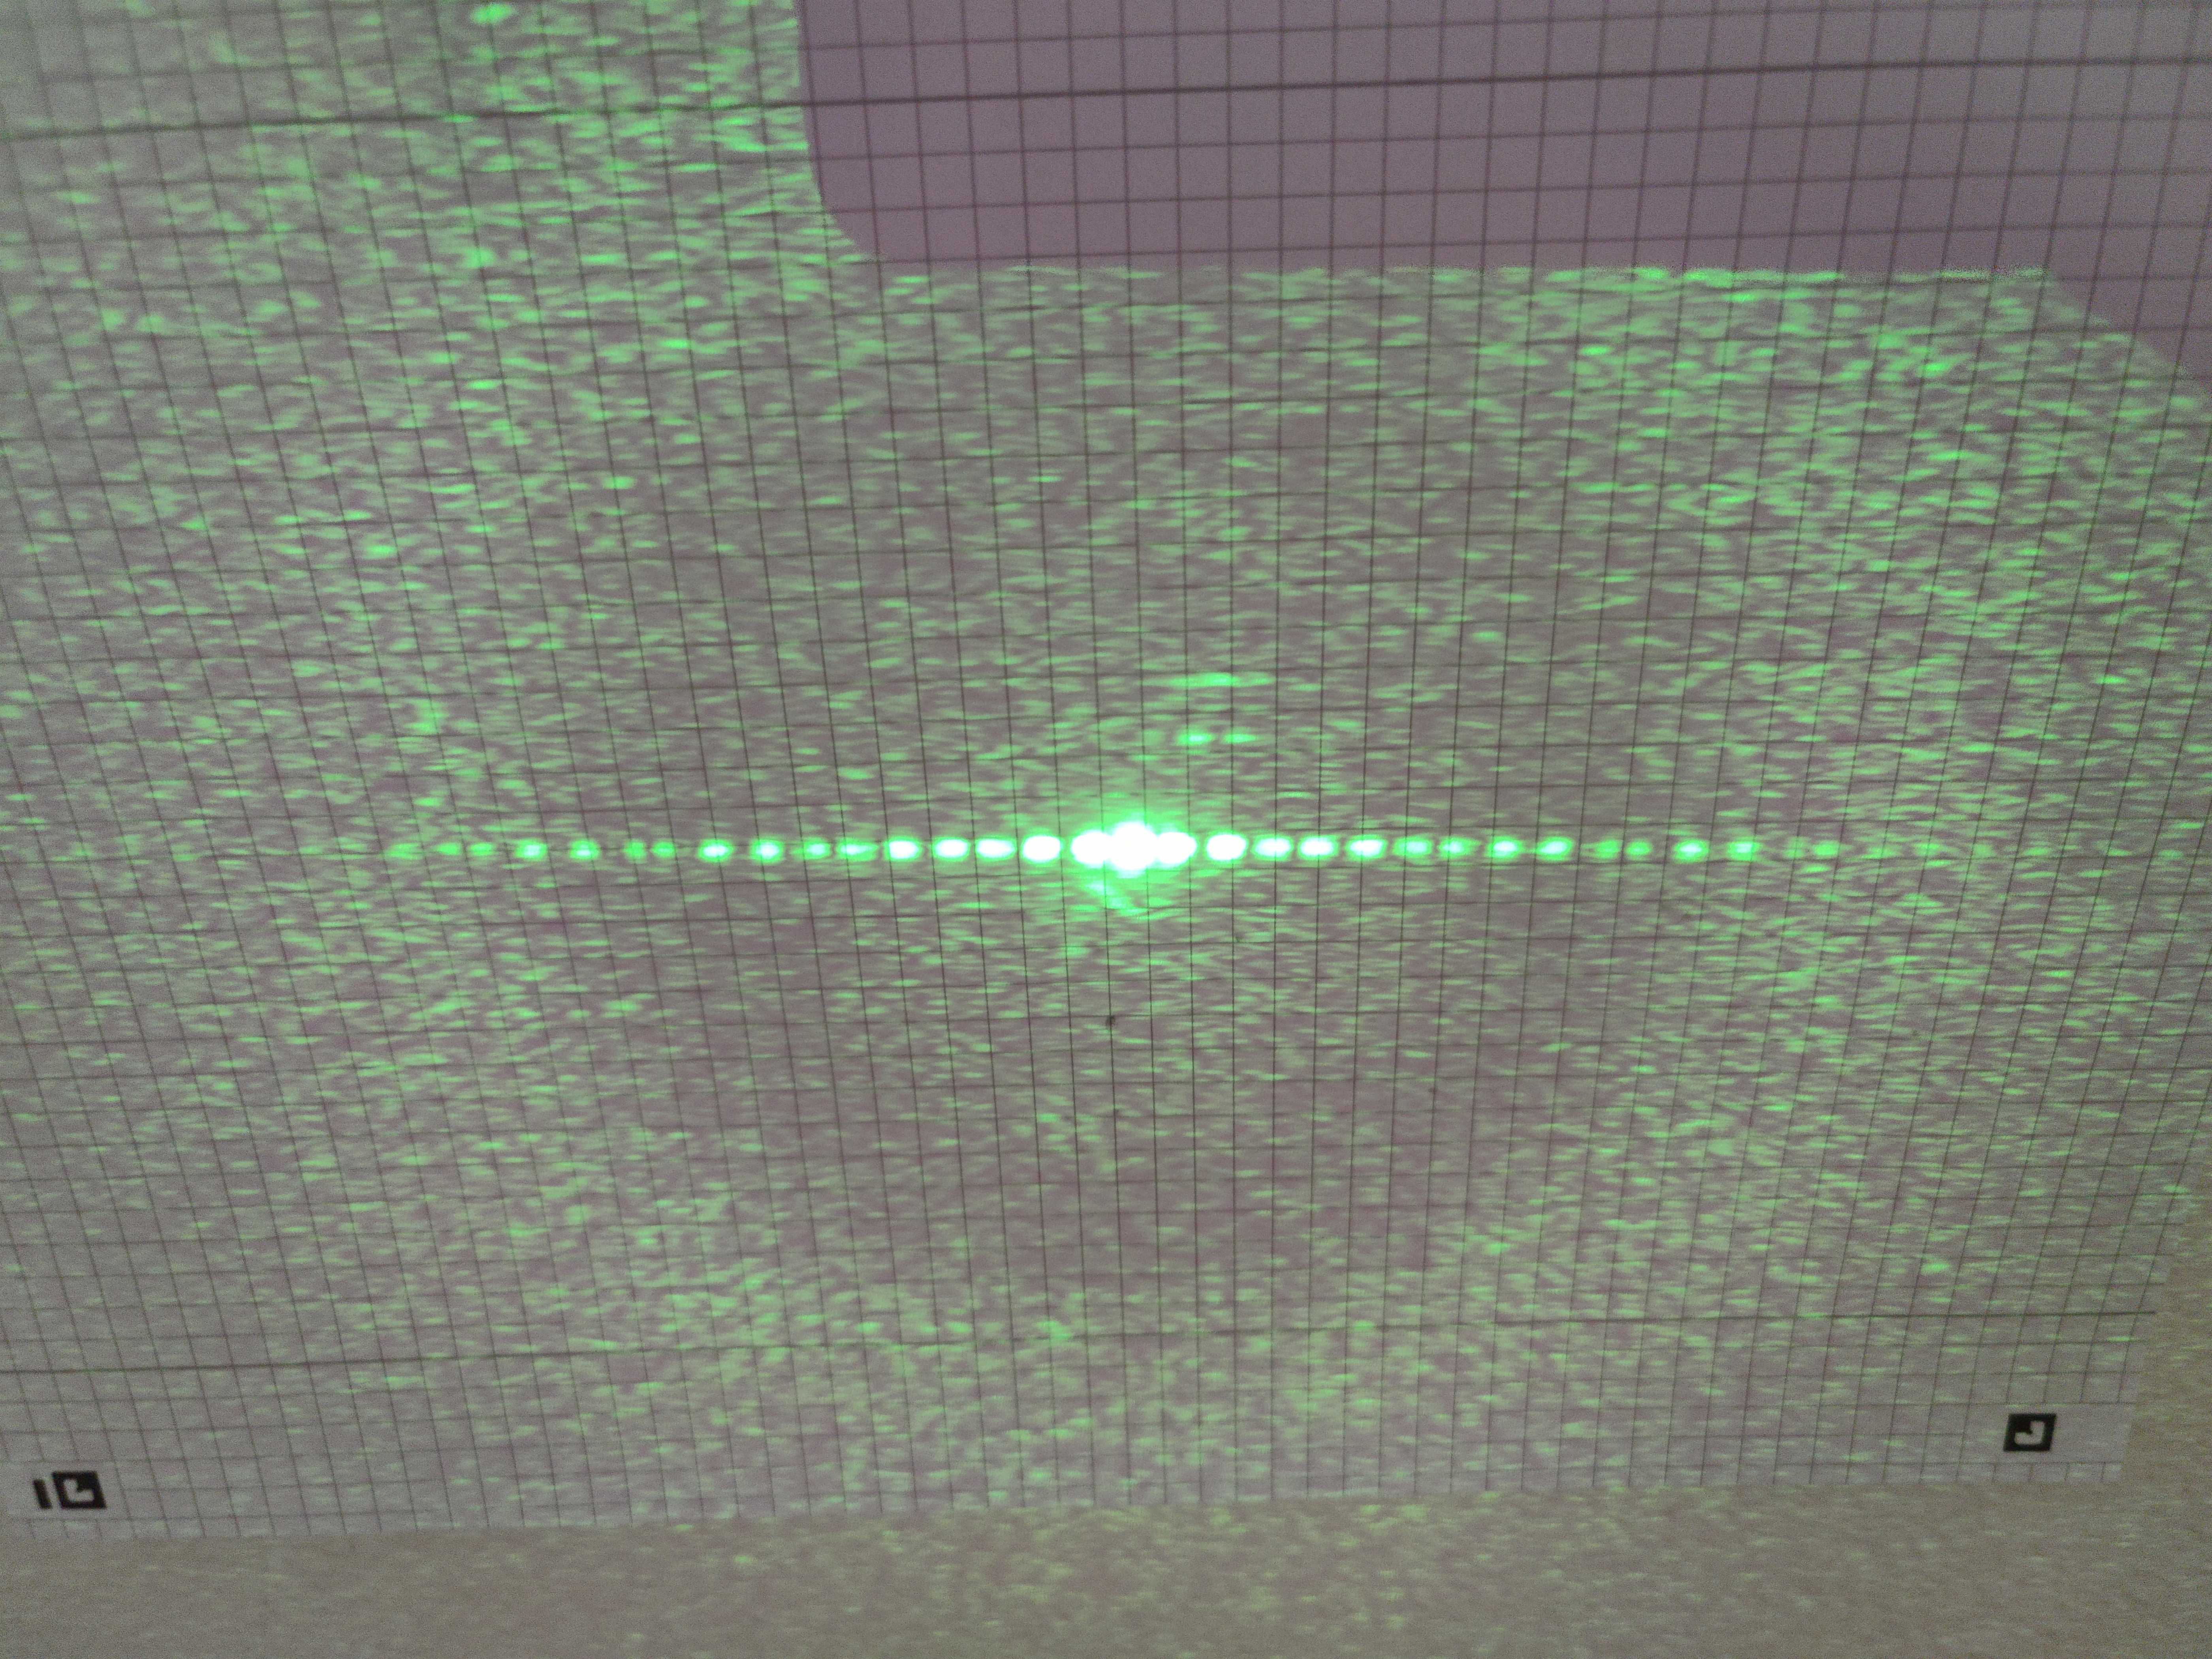
\includegraphics[width=\linewidth]{fig/Compressed/DS1_0_20_25.jpg}
        \caption{Interferenzmuster des Doppelspalts 1}
        \label{fig:DS_1_interferenzmuster}
        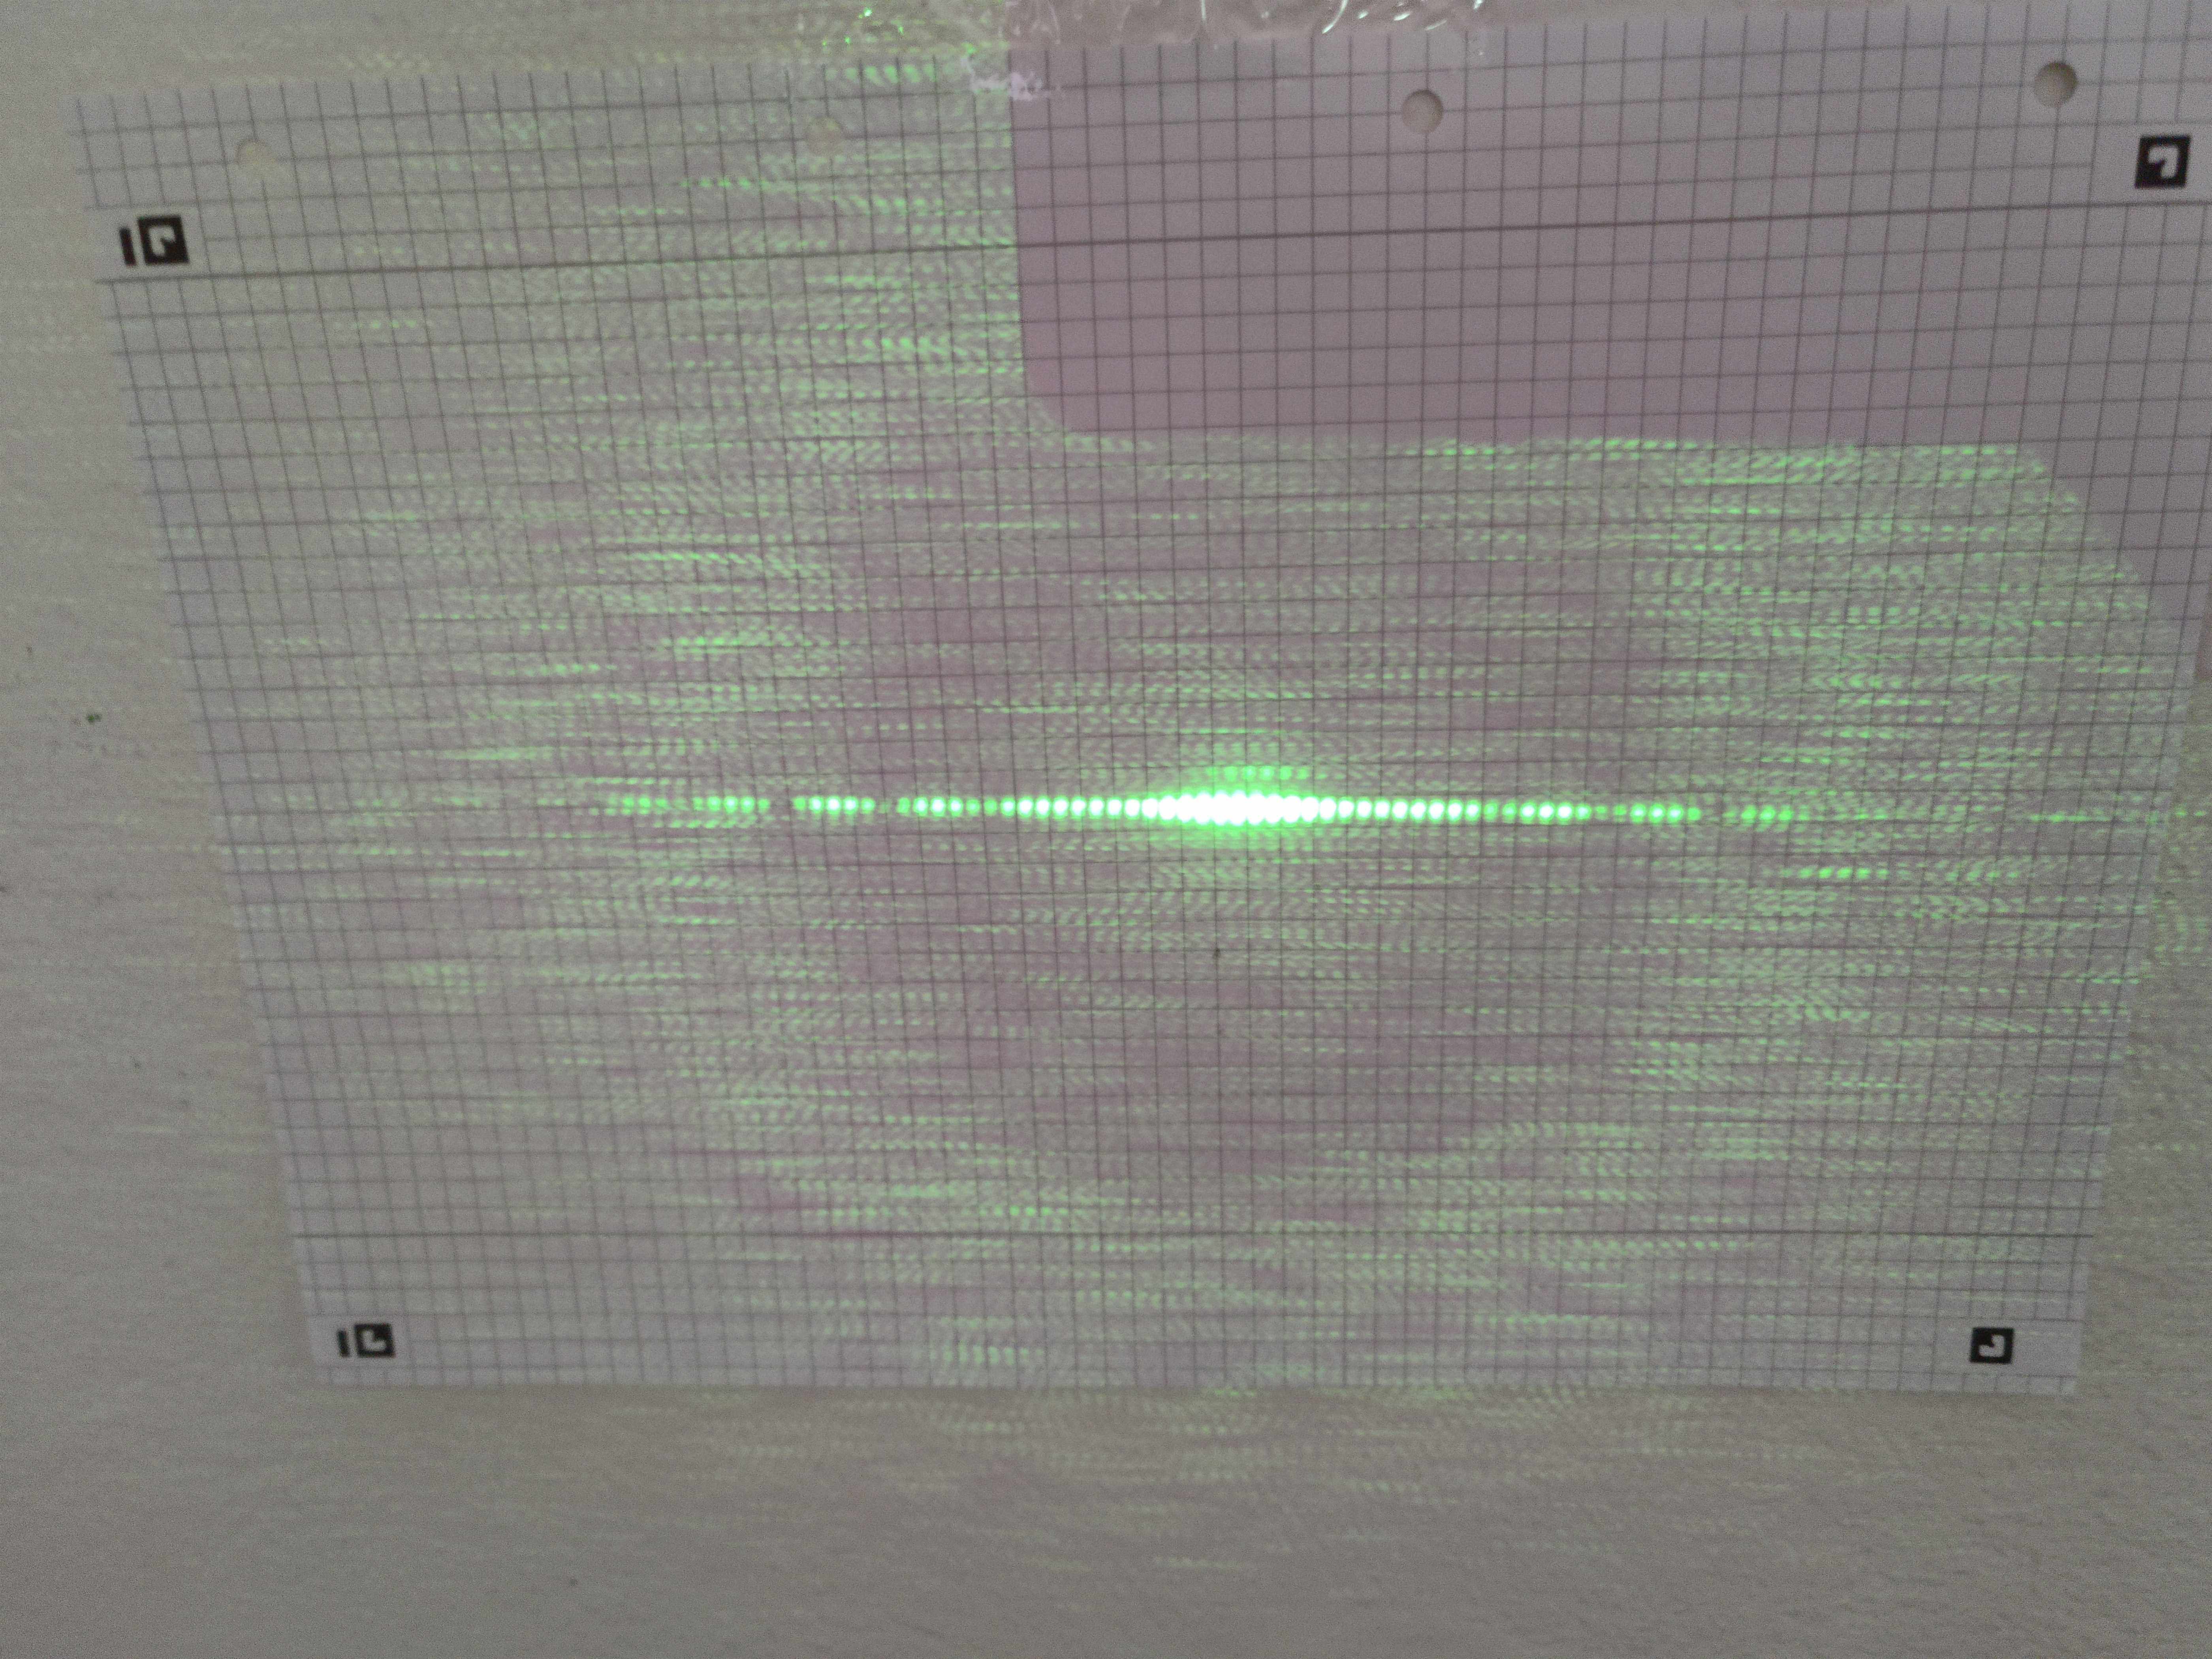
\includegraphics[width=\linewidth]{fig/Compressed/DS3_0_10_5.jpg}
        \caption{Interferenzmuster des Doppelspalts 3}
        \label{fig:DS_3_interferenzmuster}
    \end{minipage}%
    \hspace*{\fill}
    \begin{minipage}[t]{0.45\linewidth}
        \centering
        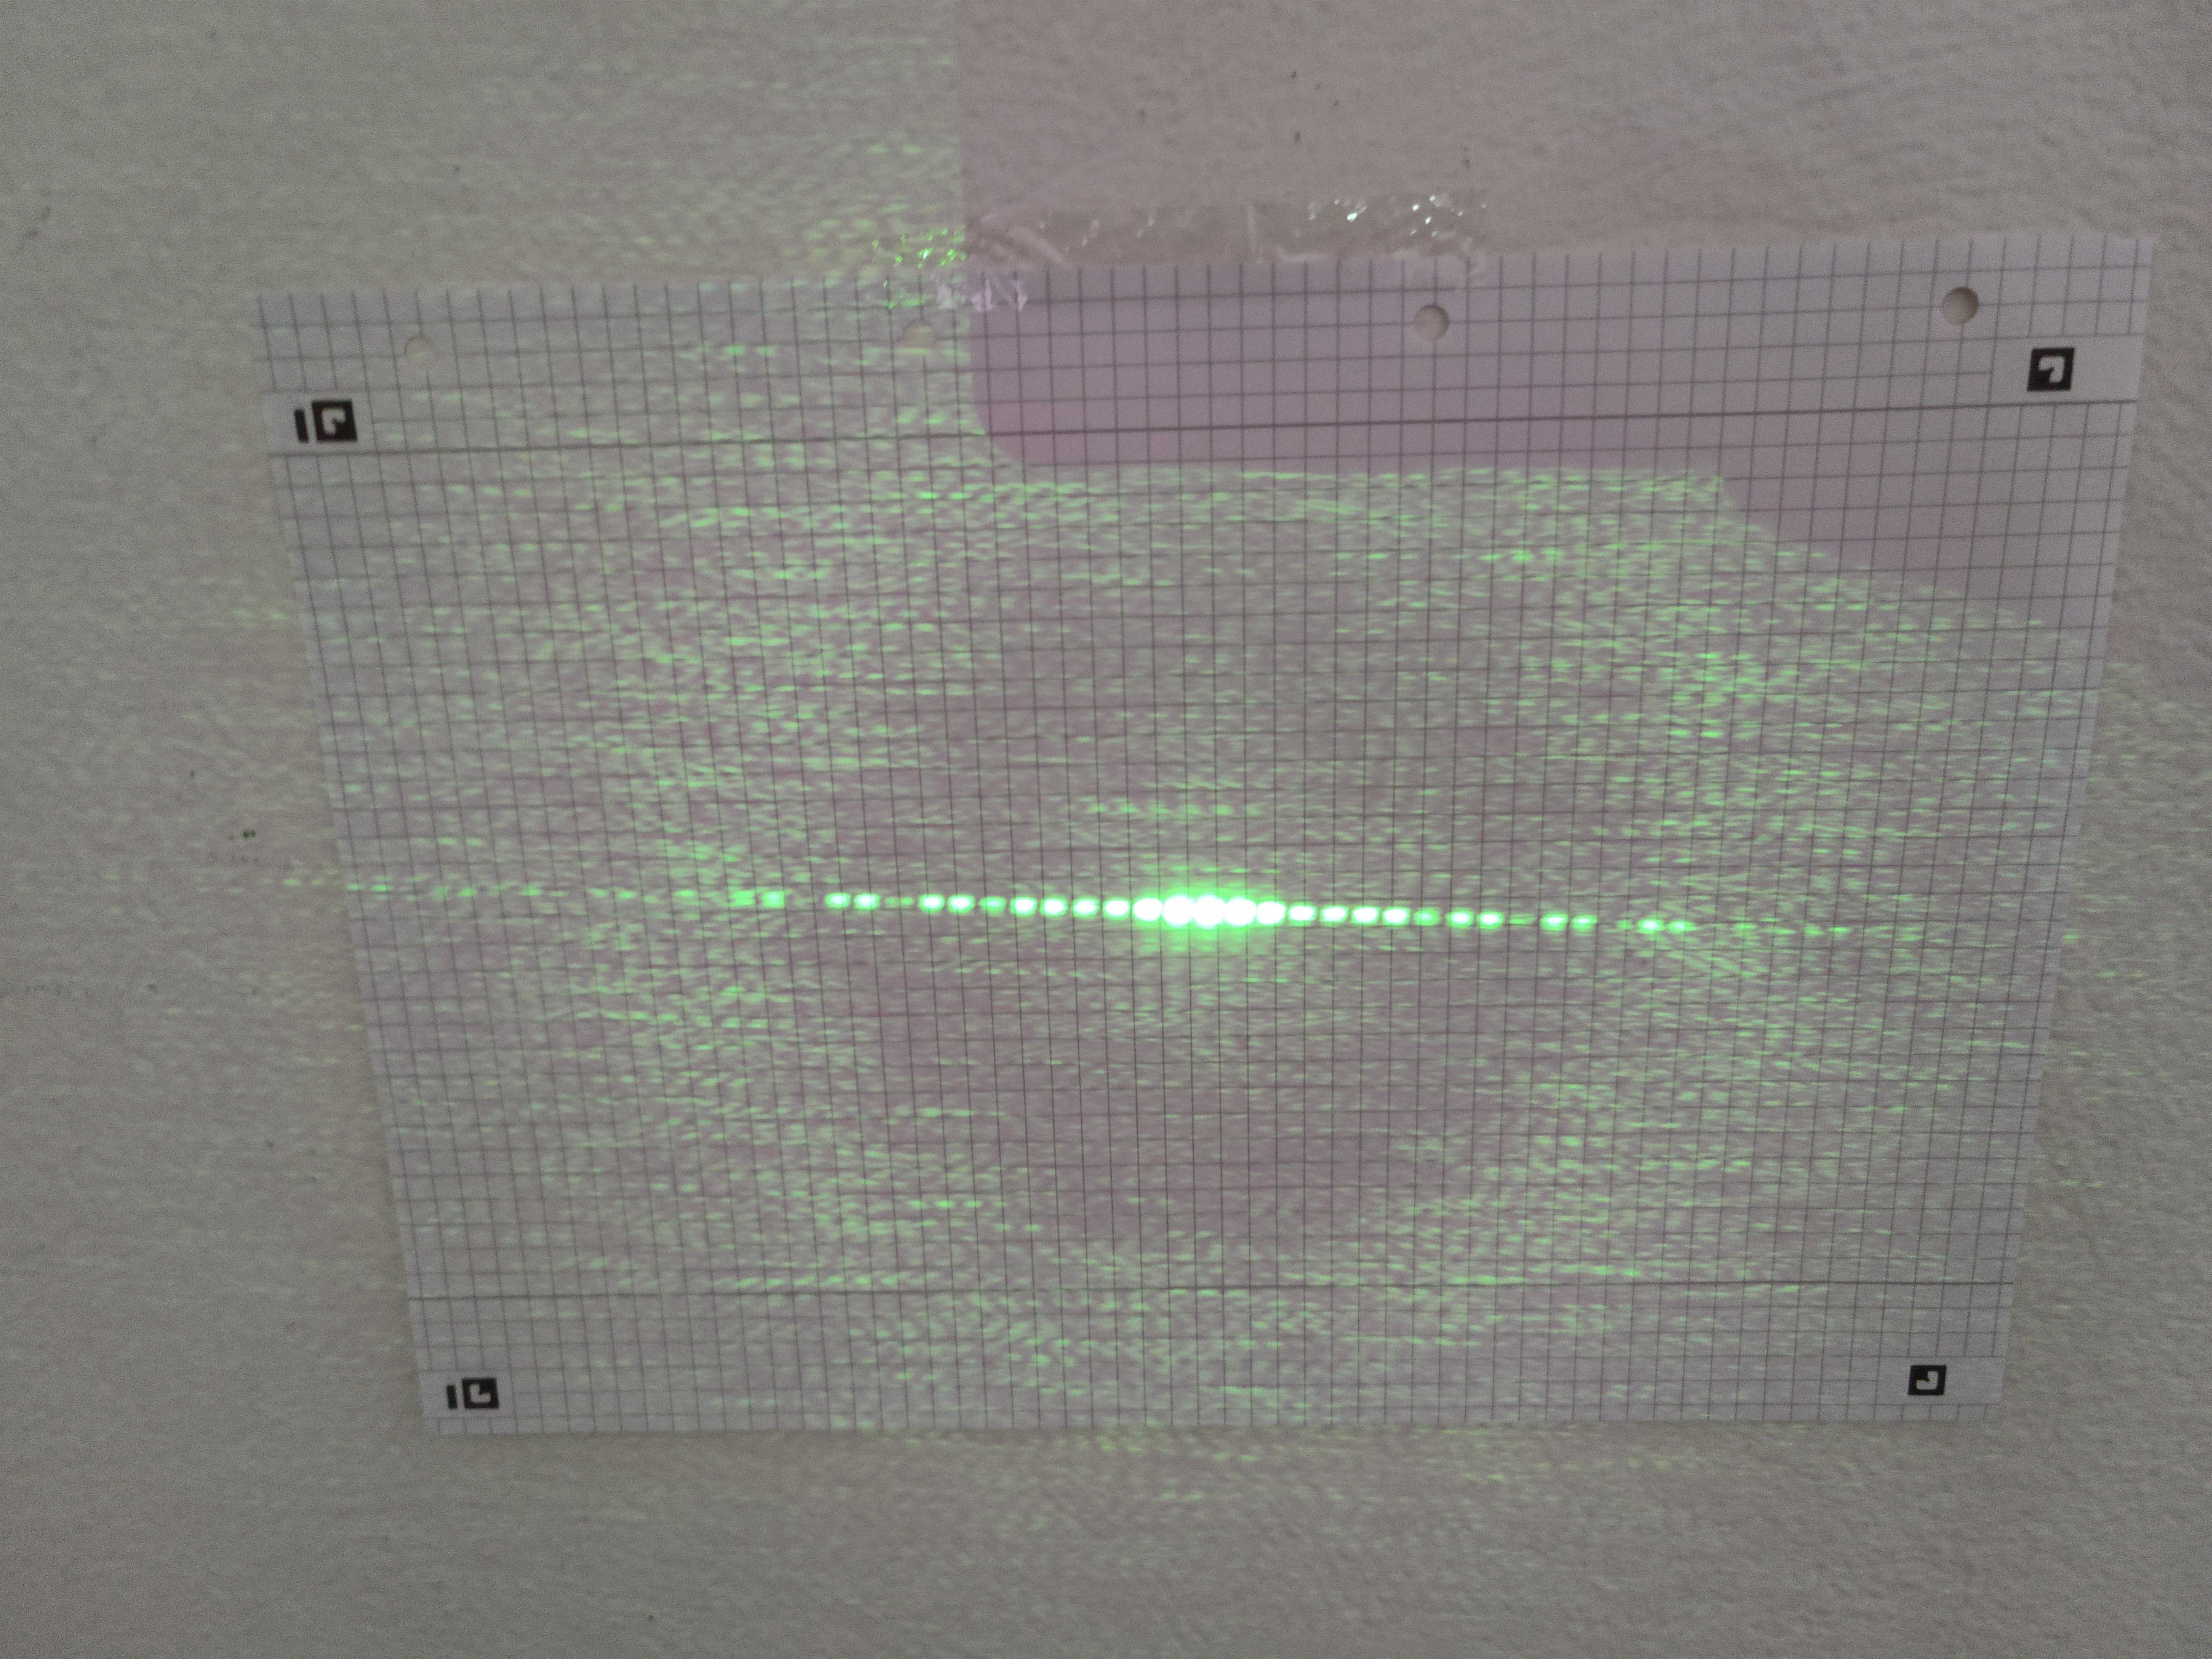
\includegraphics[width=\linewidth]{fig/Compressed/DS2_0_10_25.jpg}
        \caption{Interferenzmuster des Doppelspalts 2}
        \label{fig:DS_2_interferenzmuster}
        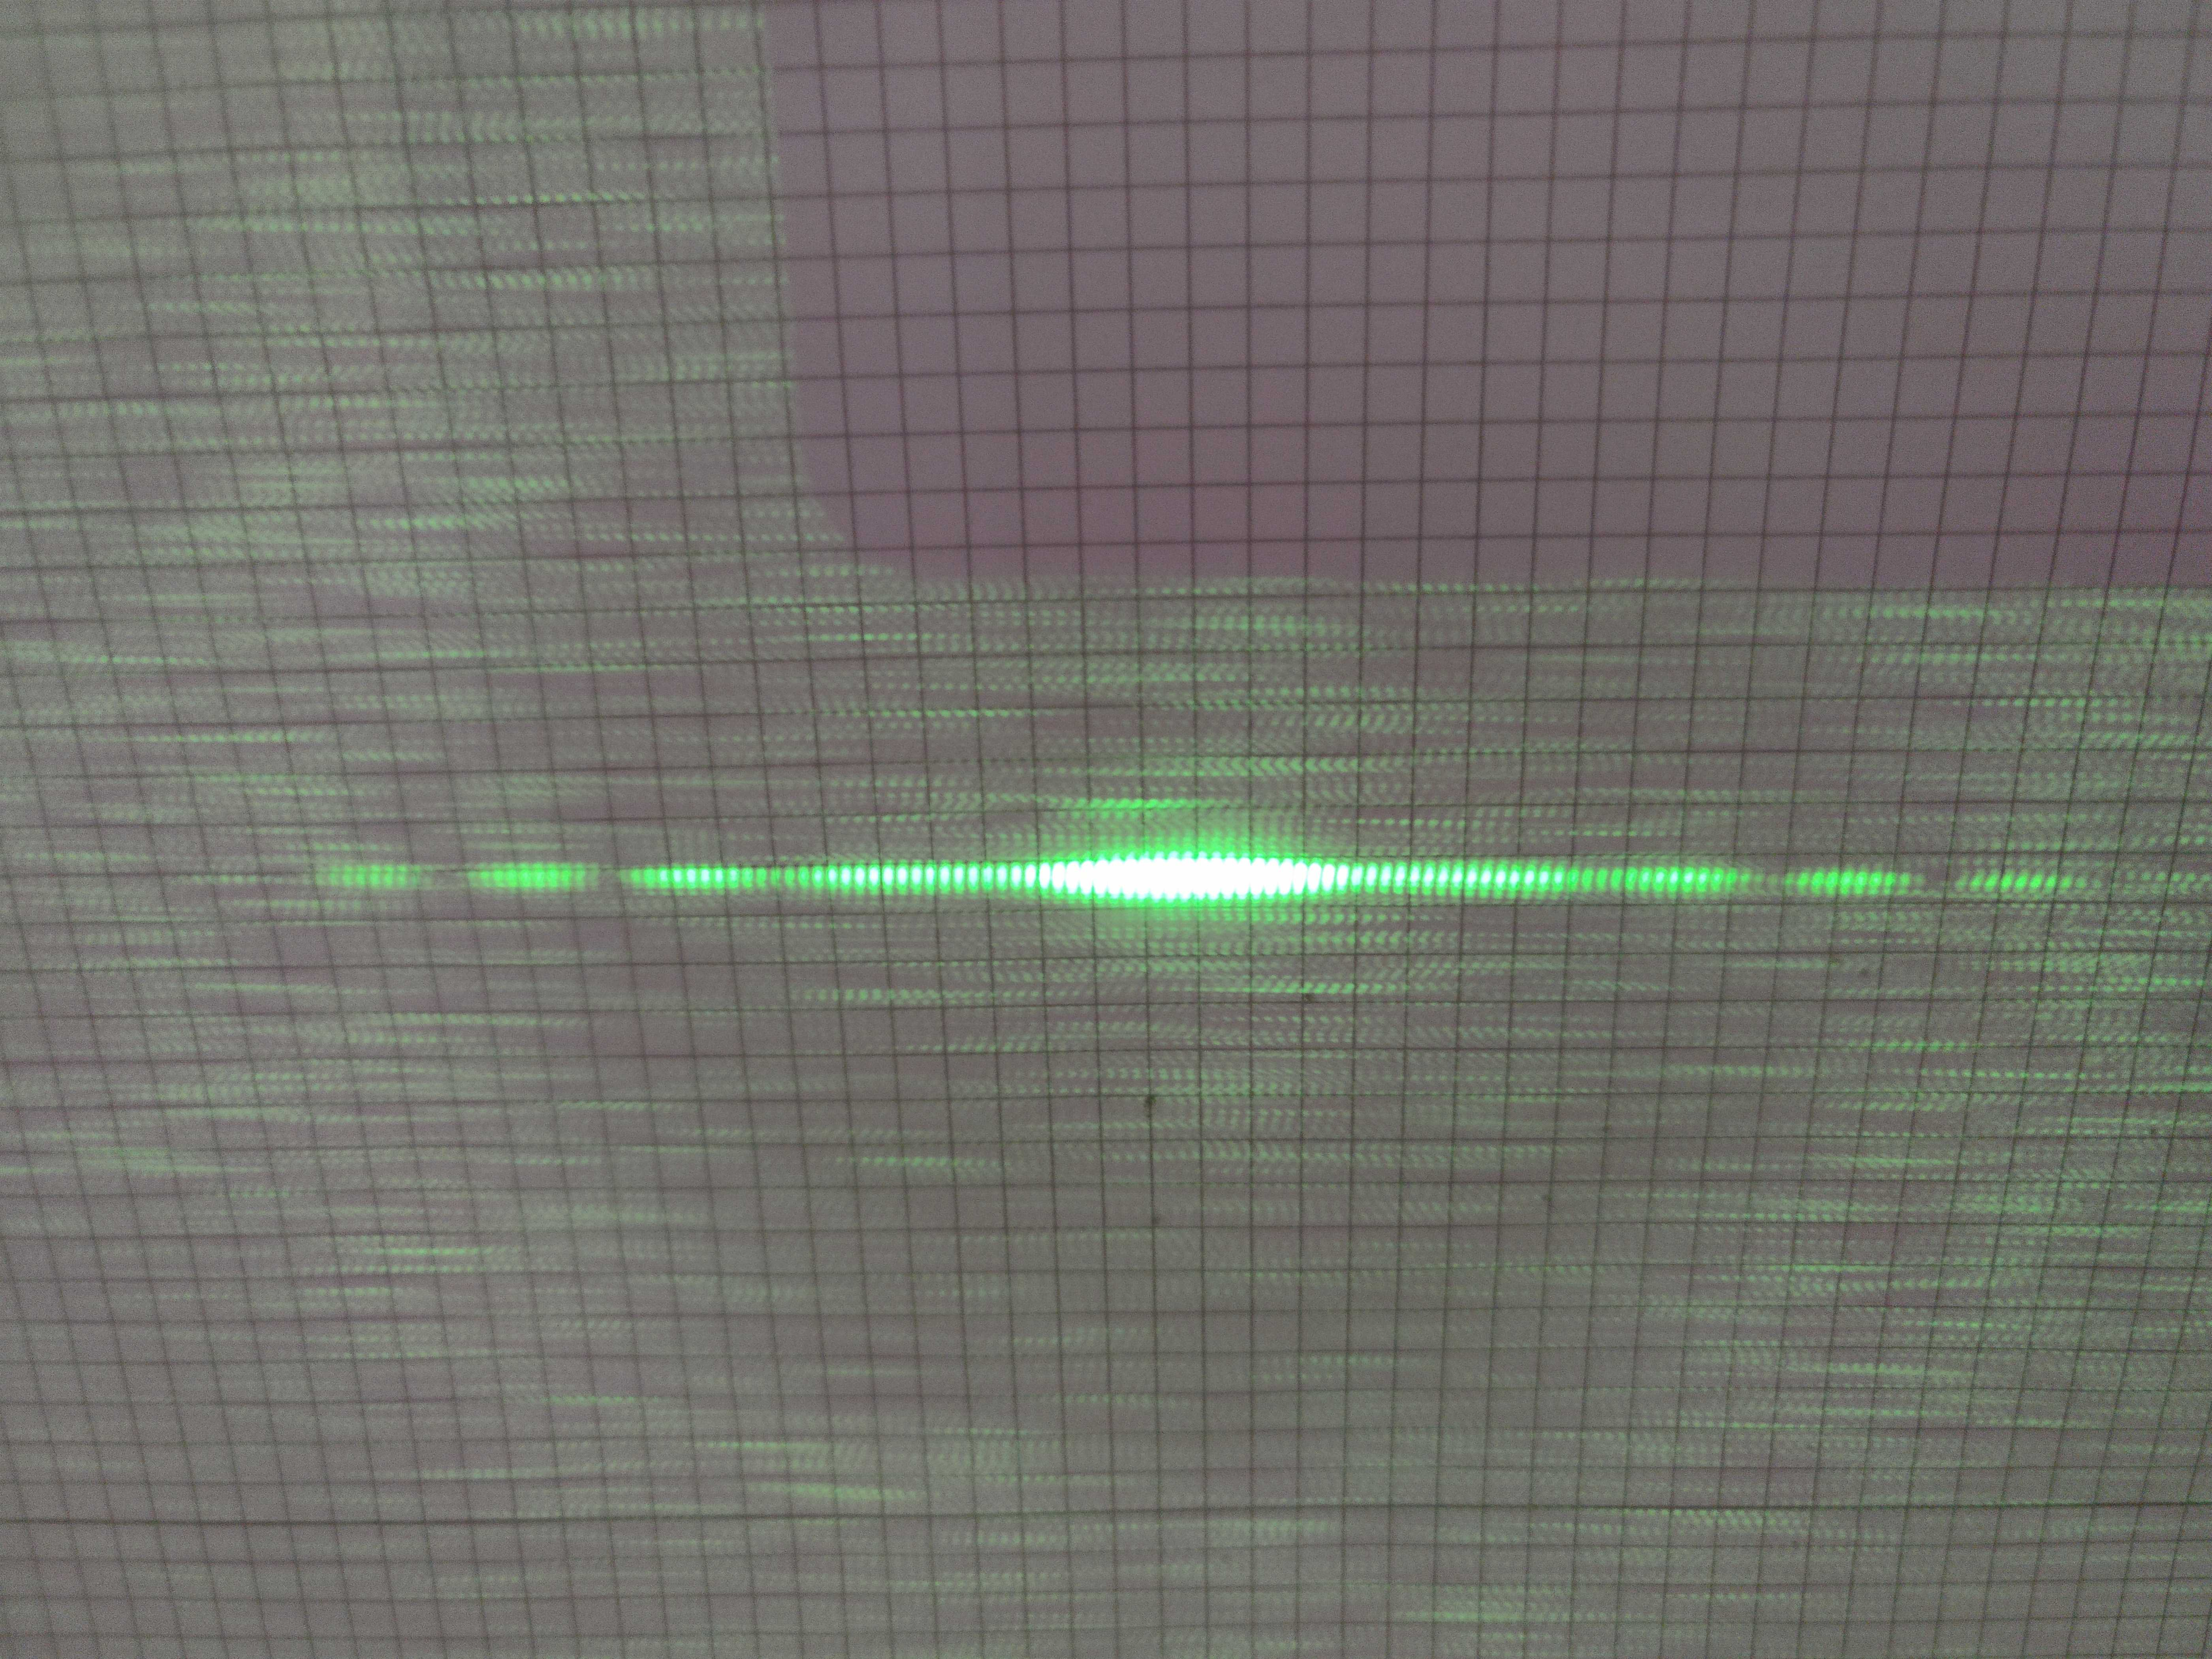
\includegraphics[width=\linewidth]{fig/Compressed/DS4_0_11.jpg}
        \caption{Interferenzmuster des Doppelspalts 4}
        \label{fig:DS_4_interferenzmuster}
    \end{minipage}
\end{figure}
\setcaphanging
%
Neben der fotografischen Dokumentation werden auch die Abstände der Maxima mittels Lineal vermessen. Die Messungen ergeben die in \autoref{tab:messwerte_doppelspalten} angeführten Werte.

%? Auf meinem laptop geht glaub i tabularray ned gescheit aber vermultich is es nur ein user error :D
\begin{table}[H]
    \centering
    \begin{samepage}
        \caption[Messwerte Doppelspalten]{Messwerte der Doppelspalten. Unsicherheit der Messung: $\Delta l_i = \SI{0.5}{\milli\meter}$}
        \label{tab:messwerte_doppelspalten}
        \begin{tblr}{colspec={Q S[table-format=2.1] S[table-format=2.1] S[table-format=2.1] S[table-format=2.1]}, row{1}={guard}}
            $i$ & $l_{1,i}$ / \unit{\milli\meter} & $l_{2,i}$ / \unit{\milli\meter} & $l_{3,i}$ / \unit{\milli\meter} & $l_{4,i}$ / \unit{\milli\meter} \\
            0   & 0.0                             & 0.0                             & 0.0                             & 0.0                             \\
            1   & 5.0                             & 5.0                             & 2.5                             & 1.5                             \\
            2   & 11.0                            & 11.0                            & 8.0                             & 2.5                             \\
            3   & 16.0                            & 16.0                            & 10.5                            & 4.0                             \\
            4   & 21.0                            & 22.0                            & 13.0                            & 5.5                             \\
            5   & 27.0                            & 27.0                            & 16.0                            & 6.5                             \\
            6   & 33.0                            & 32.0                            & 18.5                            & 8.0                             \\
            7   & 38.0                            & 38.0                            & 21.0                            & 9.5                             \\
            8   & 43.0                            & 43.0                            & 24.0                            & 10.5                            \\
            9   & 49.0                            & 48.0                            & 26.5                            & 12.0                            \\
            10  & 55.0                            & 54.0                            & 29.0                            & 13.5                            \\
            11  & 58.0                            & {{{-}}}                         & {{{-}}}                         & 15.0                            \\
        \end{tblr}
    \end{samepage}
\end{table}

Die eben beschriebene Messung wird nun in analoger Weise nochmals mit dem Gitter durchgeführt (\autoref{fig:gitter_interferenzmuster}). Die Messungen ergeben die in \autoref{tab:messwerte_gitter} angeführten Werte. Dabei bleibt der Abstand zum Schirm $l_\text{Schirm} = \SI{2520(5)}{\milli\meter}$ konstant.

\setcapindent{0pt}
\begin{figure}[H]
    \centering
    \begin{minipage}[t]{0.45\linewidth}
        \centering
        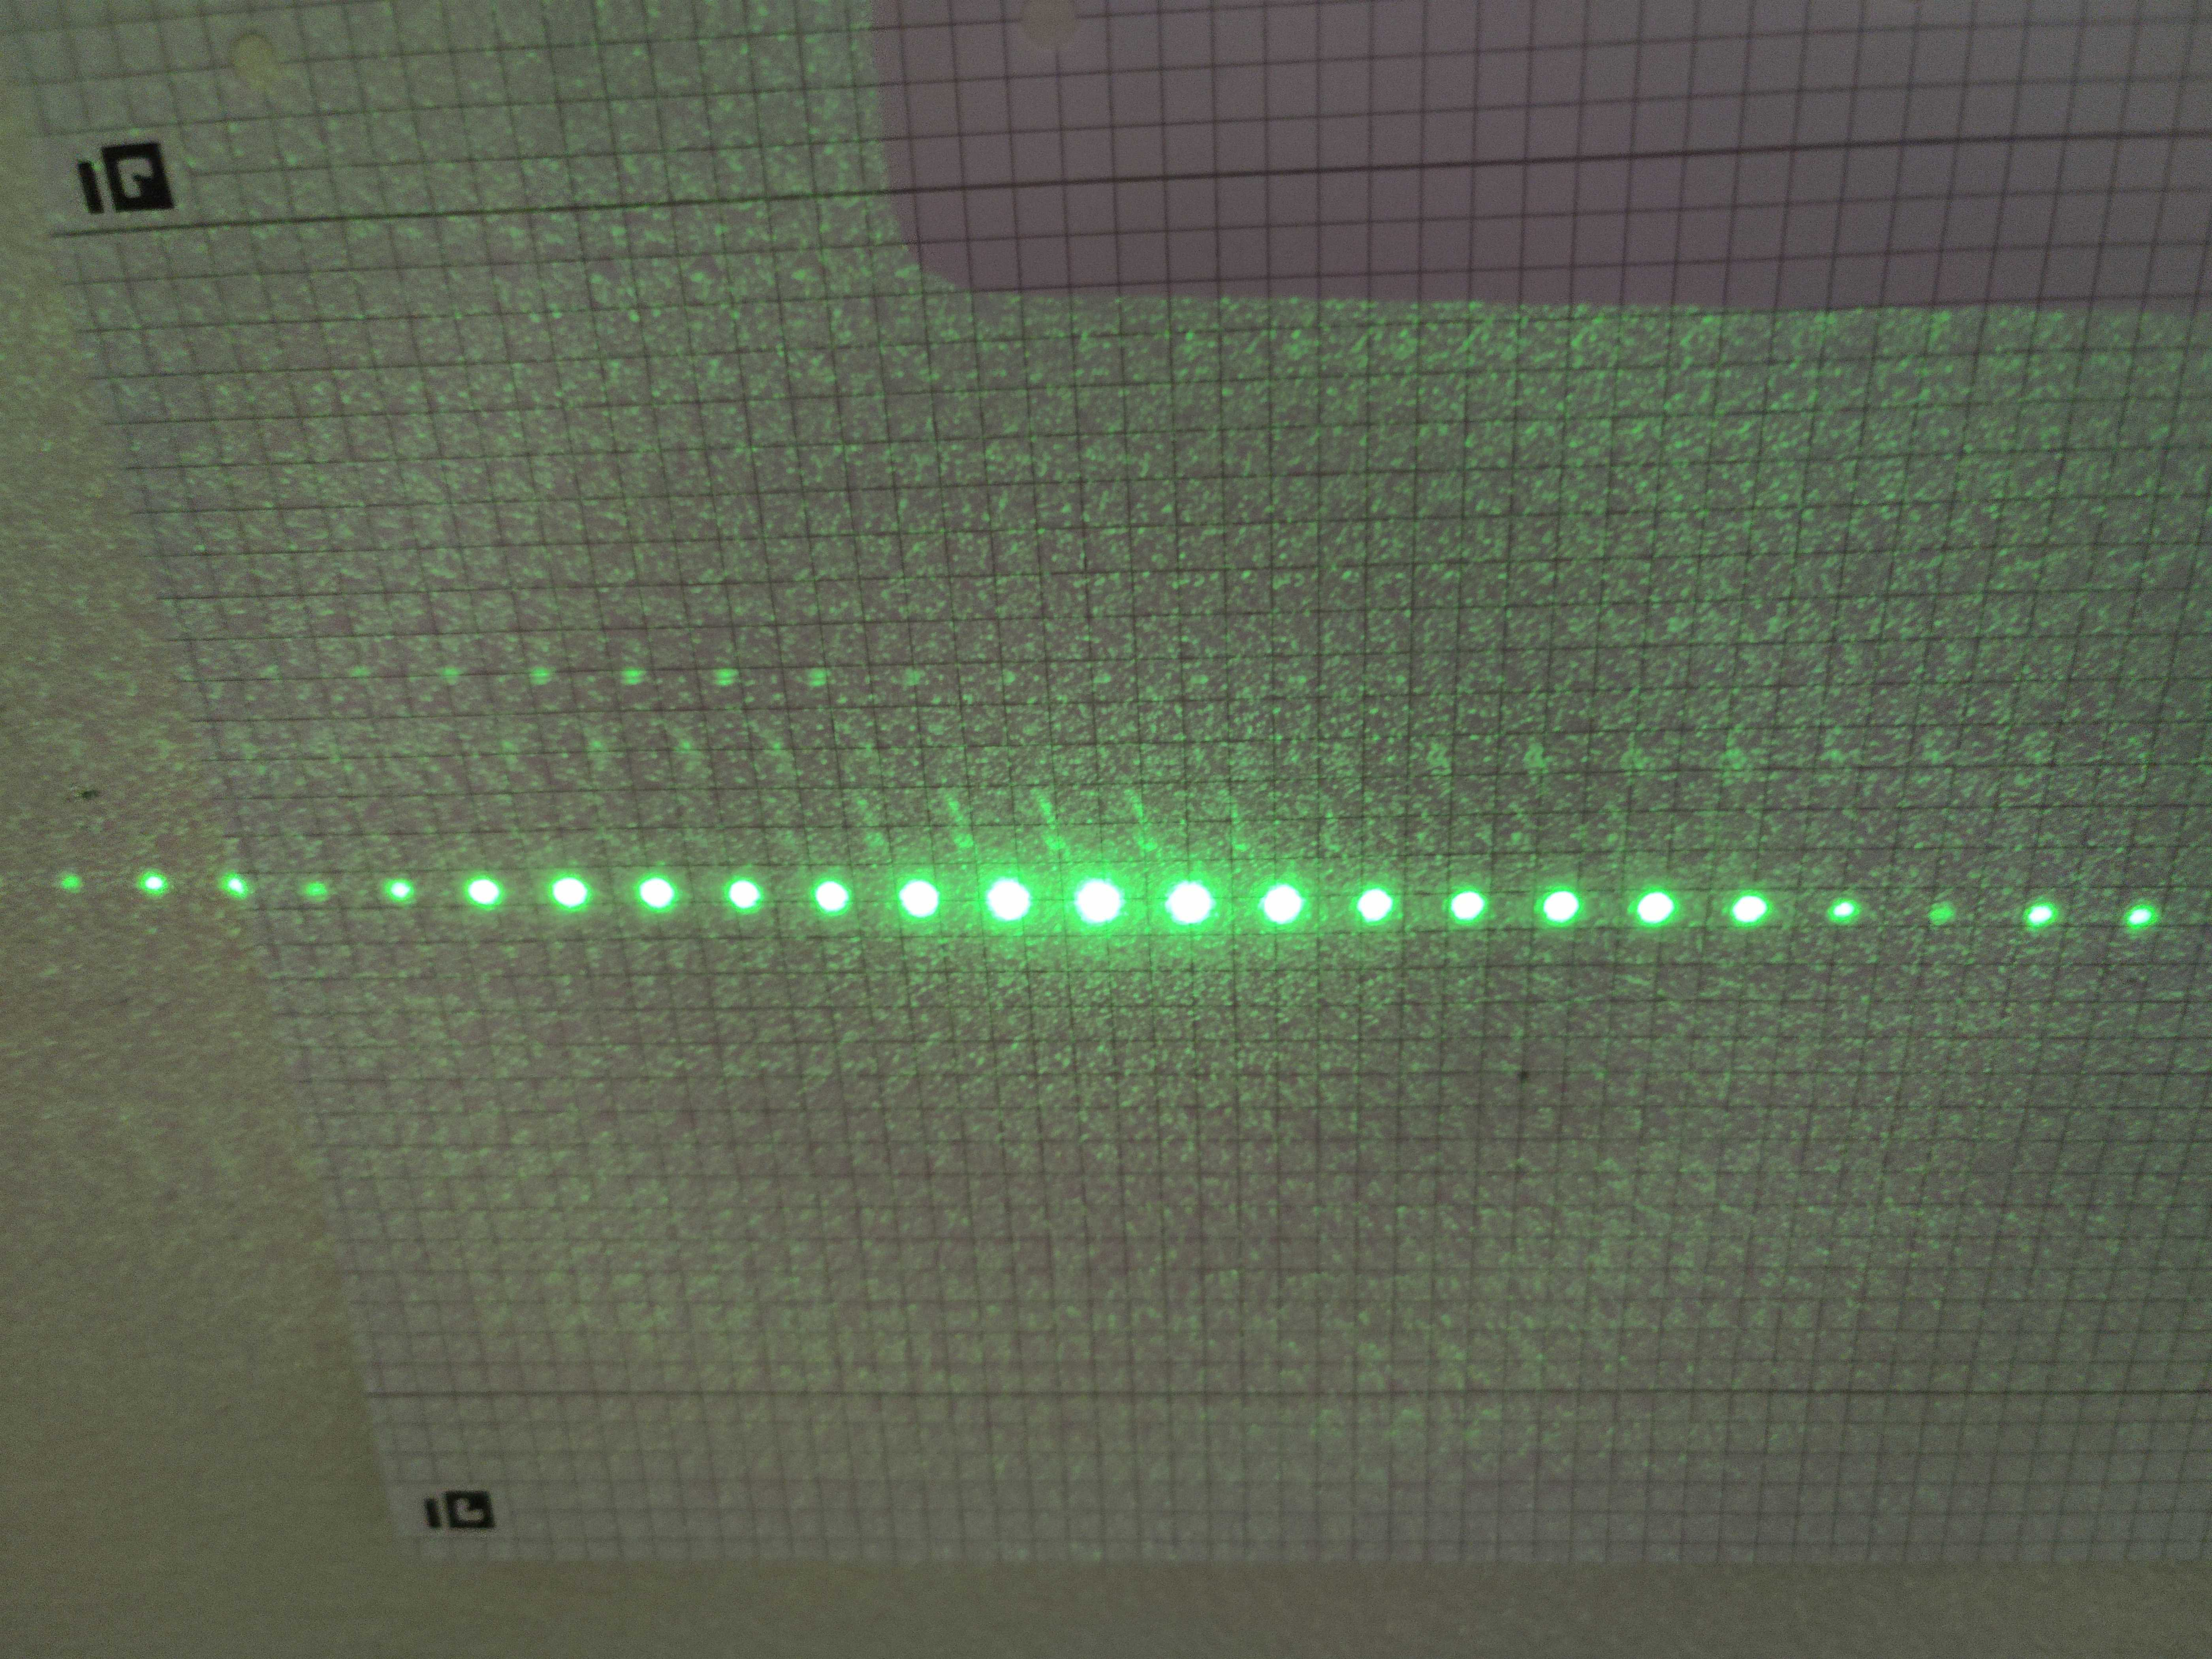
\includegraphics[width=\linewidth]{fig/Compressed/Gitter_8_per_mm.jpg}
    \end{minipage}%
    \hspace*{\fill}
    \begin{minipage}[t]{0.45\linewidth}
        \centering
        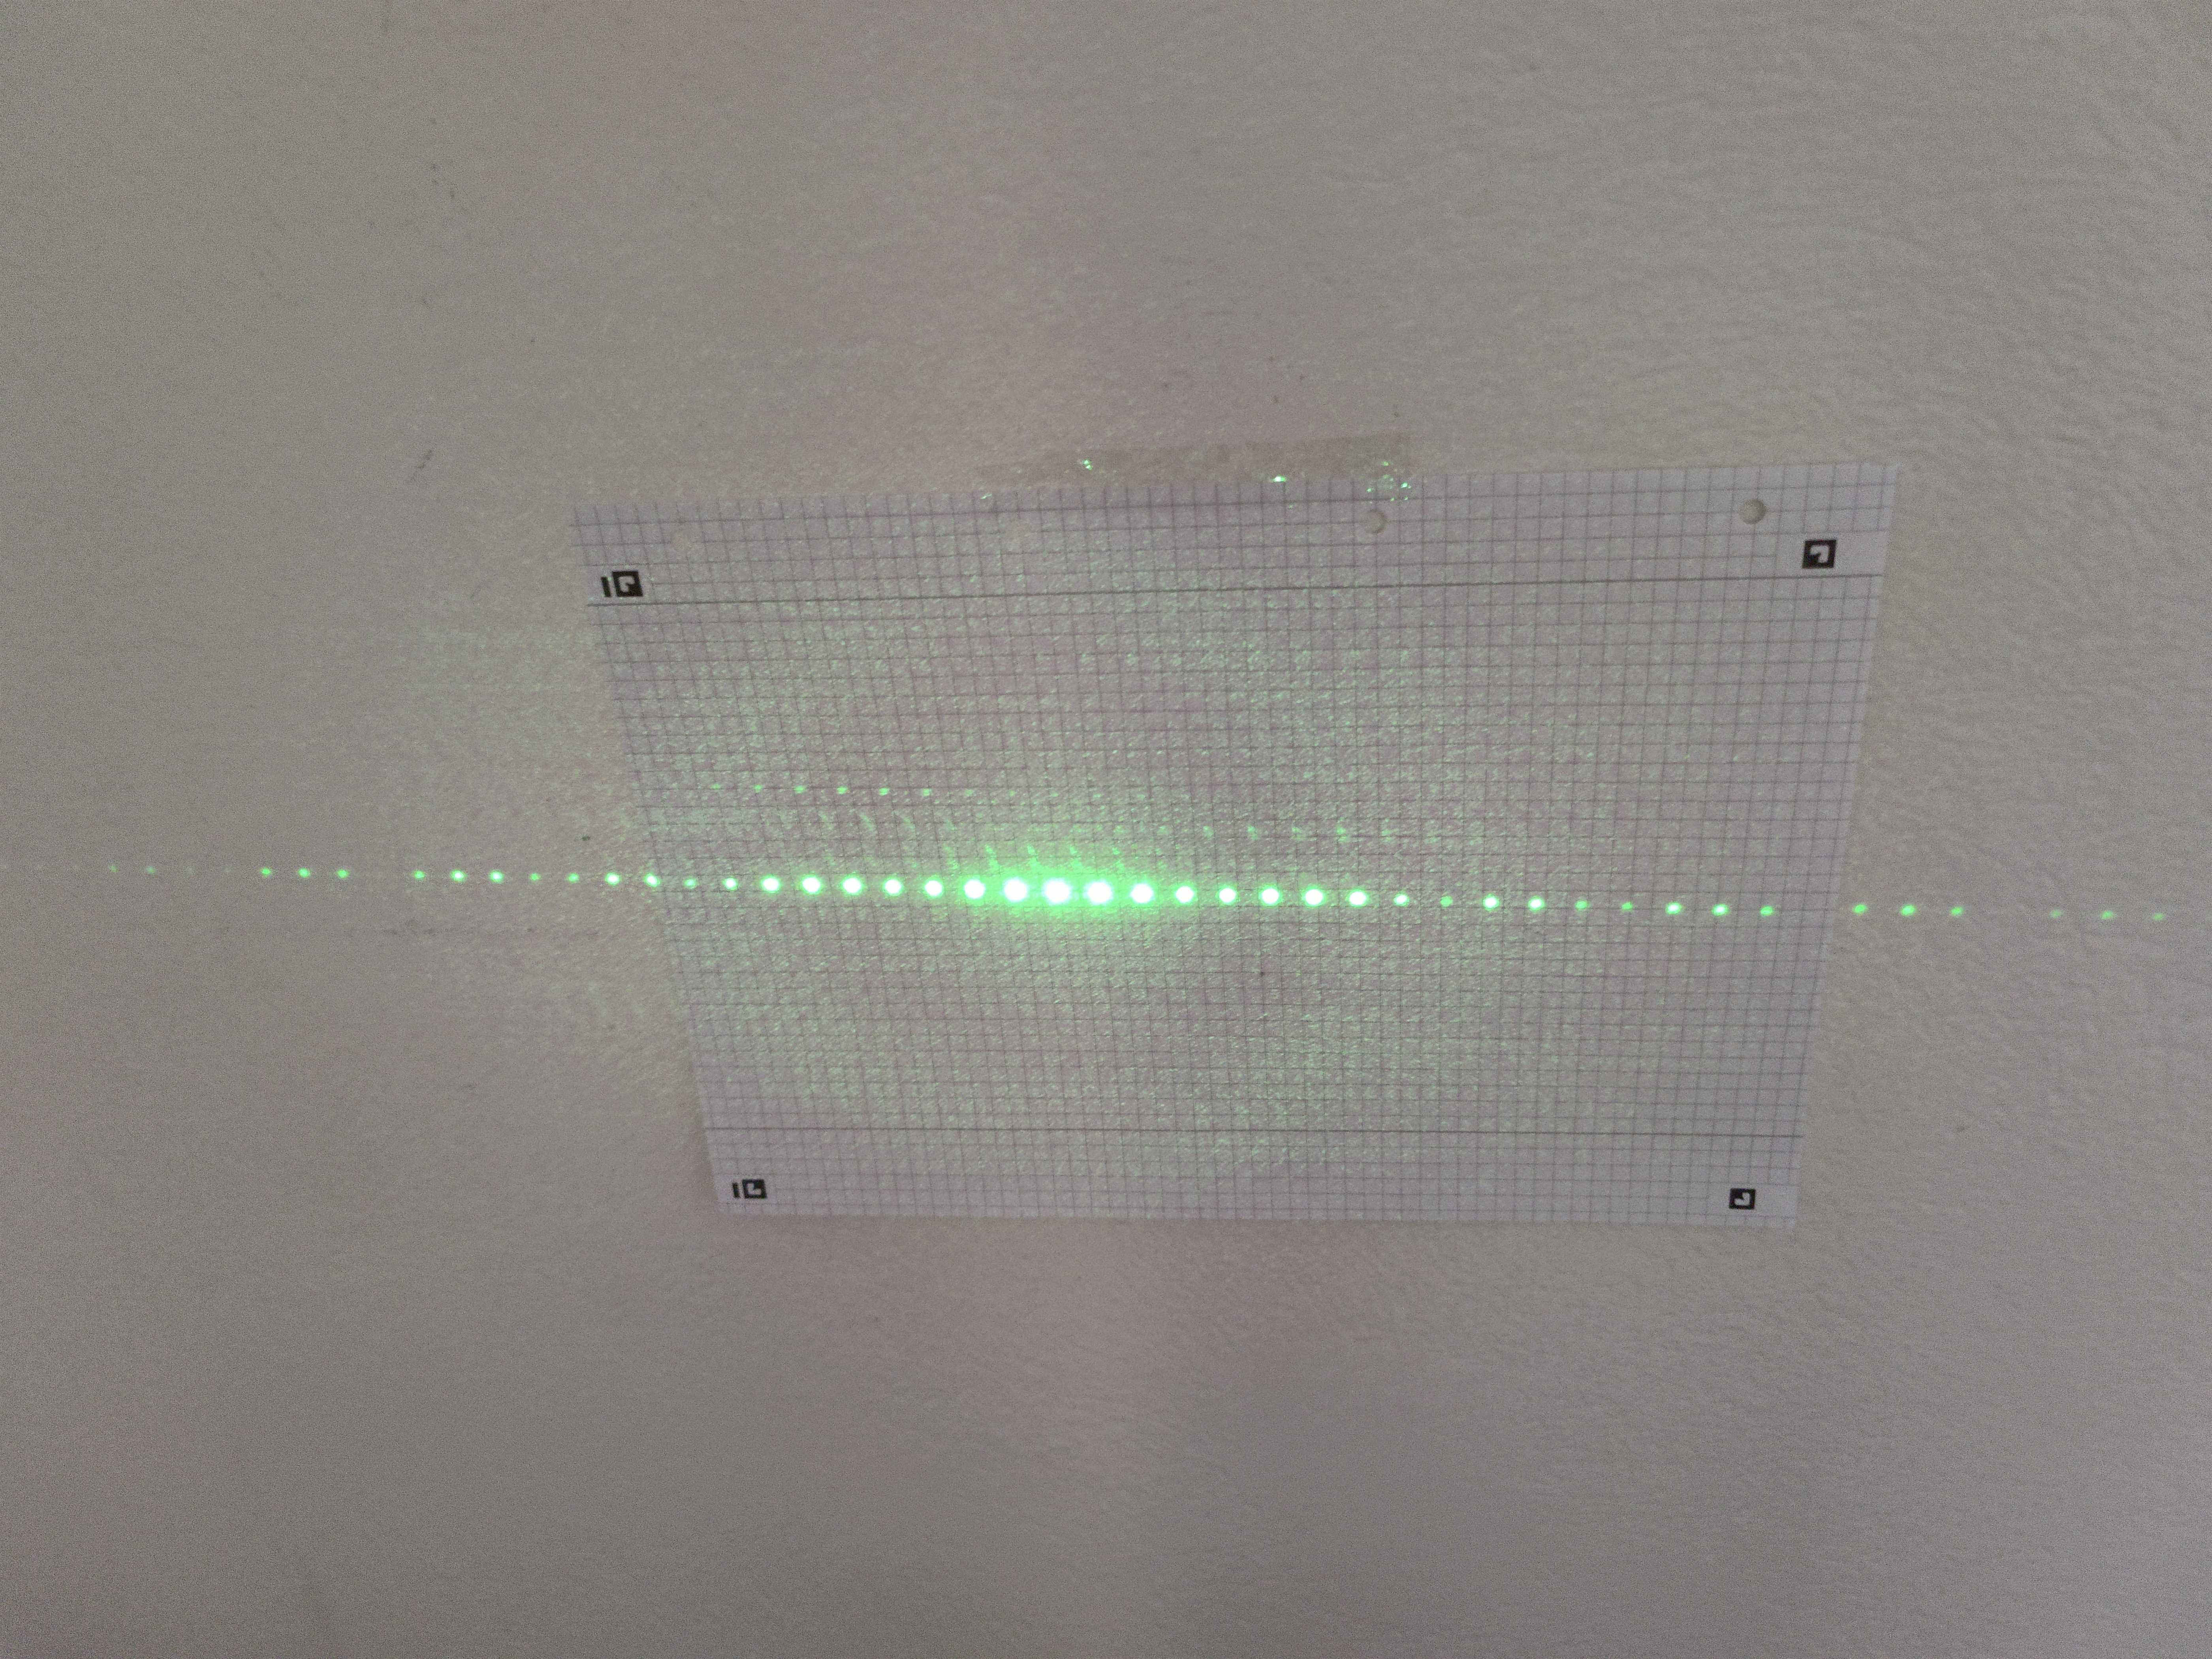
\includegraphics[width=\linewidth]{fig/Compressed/Gitter_8_per_mm_overview.jpg}
    \end{minipage}
    \caption[Interferenzmuster des Gitters]{Interferenzmuster des Gitters mit Gitterkonstante $g=\SI{8}{'\per\milli\meter}$. Links: Nahaufnahme, rechts: Übersicht über das gesamte Interferenzmuster.}
    \label{fig:gitter_interferenzmuster}
\end{figure}
\setcaphanging

\begin{table}[H]
    \centering
    \begin{samepage}
        \caption[Messwerte Gitter]{Messwerte des Gitters. Unsicherheit der Messung: $\Delta l_i = \SI{0.5}{\milli\meter}$}
        \label{tab:messwerte_gitter}
        \begin{tblr}{colspec={Q S[table-format=3.1]}, row{1}={guard}}
            $i$ / 1 & $l_i$ / \unit{\milli\meter} \\
            0       & 0.0                         \\
            1       & 11.0                        \\
            2       & 21.5                        \\
            3       & 32.5                        \\
            4       & 43.0                        \\
            5       & 53.5                        \\
            6       & 64.5                        \\
            7       & 75.0                        \\
            8       & 86.0                        \\
            9       & 97.0                        \\
            10      & 108.0                       \\
            11      & 118.0                       \\
            12      & 128.0                       \\
            13      & 139.0                       \\
            14      & 151.0                       \\
        \end{tblr}
    \end{samepage}
\end{table}


\subsection{Shearing-Interferometer}
\label{sec:durchfuehrung_shearing}

Nachdem der Versuchaufbau ordnungsgemäß hergestellt ist, wird der Laser eingeschaltet. Am optischen Ausgang am oberen Ende des Shearing-Interferometers erscheint dadurch ein streifenförmiges Interferenzmuster. Aus diesem Interfenzmuster werden der Versatz in laterale Richtung $l$, der Abstand der Interferenzstreifen $d$ und der Winkelversatz zur einfallenden Ebene $\theta$ vermessen. Vermessen wurde direkt am optischen Ausgang mit einem handelsüblichen durchsichtigen Geodreieck. Für die Längenmessung wird eine Ableseunsicherheit von \SI{0.5}{mm} angenommen, die Winkelmessung wird mit einer Ungenauigkeit von \SI{3}{\degree} abgeschätzt. Aufgrund der hohen Messungenauigkeit dieser Methodik wird die Messung zwei weitere Male wiederholt, um so zumindest eine geringfügige statistische Aussage treffen zu können. Die Messergebnisse werden notiert und tabelliert.

%!Natürlich komplett frei erfunden
\begin{table}[H]
    \centering
    \begin{samepage}
        \caption[Messung Shearing]{Gemessene Größen beim Versuchsaufbau \textit{Shearing-Interferometer} mit $i$ dem Laufindex der einzelnen Messungen, $l$ dem Versatz in laterale Richtung, $d$ dem Abstand der Interferenzstreifen $\theta$ und dem Winkelversatz zur einfallenden Ebene. Unsicherheiten: $\Delta l = \Delta s = \SI{0.5}{mm}$, $\Delta \theta = \SI{3}{\degree}$}
        \label{tab:messergebnisse_shearing}
        \begin{tblr}{colspec={Q S[table-format=2.1(1)] S[table-format=1.1(1)] S[table-format=2(1)]}, row{1}={guard}}
            $i$ / 1 & $l$ / \unit{\milli\meter} & $d$ / \unit{\milli\meter} & $\theta$ / \unit{\degree} \\
            1       & 10.0(5)                   & 3.0(5)                    & 22(3)                     \\
            2       & 9.5(5)                    & 3.5(5)                    & 20(3)                     \\
            3       & 10.0(5)                   & 3.0(5)                    & 25(3)                     \\
        \end{tblr}
    \end{samepage}
\end{table}


\subsection{Polarisation}
\label{sec:durchfuehrung_polarisation}

Der Strahl wird für den ersten Unterpunkt dieses Versuchs durch zwei Polarisationsfilter geführt. Für den ersten der beiden Filter wurde \SI{70}{\degree} als Ausgangswinkel gewählt, der zweite wird im folgenden Versuch einmal um \SI{360}{\degree} gedreht, wobei die Ausgangsstellung hier so gewählt wird, dass zuerst die höchste Lichtintensität am Messgerät abgelesen werden kann. So stehen die Polarisationsfilter gleich, dies ist bei \SI{330}{\degree} des zweiten Filters der Fall.
Die Messung wurde zweimal durchgeführt und die gemessenen Werte des Lichtintensitätsmesser sind in \autoref{tab:messwerte_polarisation} angeführt.

%! Caption is scheiße und zu klein
\begin{longtblr}[
        caption = {Messwerte nach Durchgang durch zwei Polarisationsfilter. Winkel des ersten Filters: \SI{70}{\degree}, Winkel des zweiten Filters $\alpha$ mit $\Delta \alpha = \SI{3}{\degree}$, Intensität $I_i$ mit Index $i=1 \mathcomma 2$ für die beiden nacheinanderfolgenden Messungen, $\Delta I_i$ Unsicherheit der Messung.},
        label = {tab:messwerte_polarisation}]{
        colspec={S[table-format=3] S[table-format=4] S[table-format=2] S[table-format=4] S[table-format=2]}}
    {{{$\alpha$}}} & {{{$I_1$ / \unit{\lux}}}} & {{{$\Delta I_1$ / \unit{\lux}}}} & {{{$I_2$ / \unit{\lux}}}} & {{{$\Delta I_2$ / \unit{\lux}}}} \\
    330            & 1020                      & 50                               & 1070                      & 50                               \\
    340            & 990                       & 50                               & 1050                      & 50                               \\
    350            & 910                       & 40                               & 960                       & 40                               \\
    0              & 780                       & 40                               & 820                       & 40                               \\
    10             & 610                       & 30                               & 640                       & 30                               \\
    20             & 440                       & 30                               & 450                       & 30                               \\
    30             & 270                       & 20                               & 280                       & 20                               \\
    40             & 130                       & 20                               & 140                       & 20                               \\
    50             & 30                        & 20                               & 30                        & 20                               \\
    60             & 0                         & 10                               & 0                         & 10                               \\
    70             & 20                        & 20                               & 20                        & 20                               \\
    80             & 100                       & 20                               & 110                       & 20                               \\
    90             & 230                       & 20                               & 250                       & 20                               \\
    100            & 390                       & 30                               & 410                       & 30                               \\
    110            & 570                       & 30                               & 600                       & 30                               \\
    120            & 750                       & 40                               & 790                       & 40                               \\
    130            & 890                       & 40                               & 940                       & 40                               \\
    140            & 1000                      & 50                               & 1040                      & 50                               \\
    150            & 1040                      & 50                               & 1090                      & 50                               \\
    160            & 1020                      & 50                               & 1070                      & 50                               \\
    170            & 950                       & 40                               & 990                       & 50                               \\
    180            & 810                       & 40                               & 840                       & 40                               \\
    190            & 650                       & 40                               & 670                       & 40                               \\
    200            & 470                       & 30                               & 490                       & 30                               \\
    210            & 280                       & 20                               & 300                       & 20                               \\
    220            & 150                       & 20                               & 150                       & 20                               \\
    230            & 30                        & 20                               & 40                        & 20                               \\
    240            & 0                         & 10                               & 0                         & 10                               \\
    250            & 20                        & 20                               & 20                        & 20                               \\
    260            & 110                       & 20                               & 120                       & 20                               \\
    270            & 250                       & 20                               & 260                       & 20                               \\
    280            & 420                       & 30                               & 440                       & 30                               \\
    290            & 600                       & 30                               & 630                       & 30                               \\
    300            & 740                       & 40                               & 810                       & 40                               \\
    310            & 920                       & 40                               & 970                       & 40                               \\
    320            & 1020                      & 50                               & 1070                      & 50                               \\
    330            & 1060                      & 50                               & 1100                      & 50                               \\
\end{longtblr}


\subsection{Michelson-Interferometer}
\label{sec:durchfuehrung_michelson}

Das Michelson-Interferometer wird wie in \autoref{fig:aufbau_michelson} beschrieben in den Strahlengang eingebracht. Nun werden die beiden Spiegel des Michelson-Interfereometers so justiert, dass die beiden Strahlen, die durch die beiden Arme des Interferometers laufen, überlagert am Schirm auftreffen. Nun wird eine Sammellinse vor dem Interferometer eingebracht, dies führt zur Ausbildung von Interferenzmustern, welche in konzentrischer Anordnung abwechselnd Maxima und Minima am Schirm, aber auch am Laser aufweisen. Beispielhaft finden sich in \autoref{fig:michelson_konz_sammel} und \autoref{fig:michelson_konz_sammel_tuer} die Interferenzmuster am Schirm und neben dem Laser.

\setcapindent{0pt}
\begin{figure}[H]
    \centering
    \begin{minipage}[t]{0.45\linewidth}
        \centering
        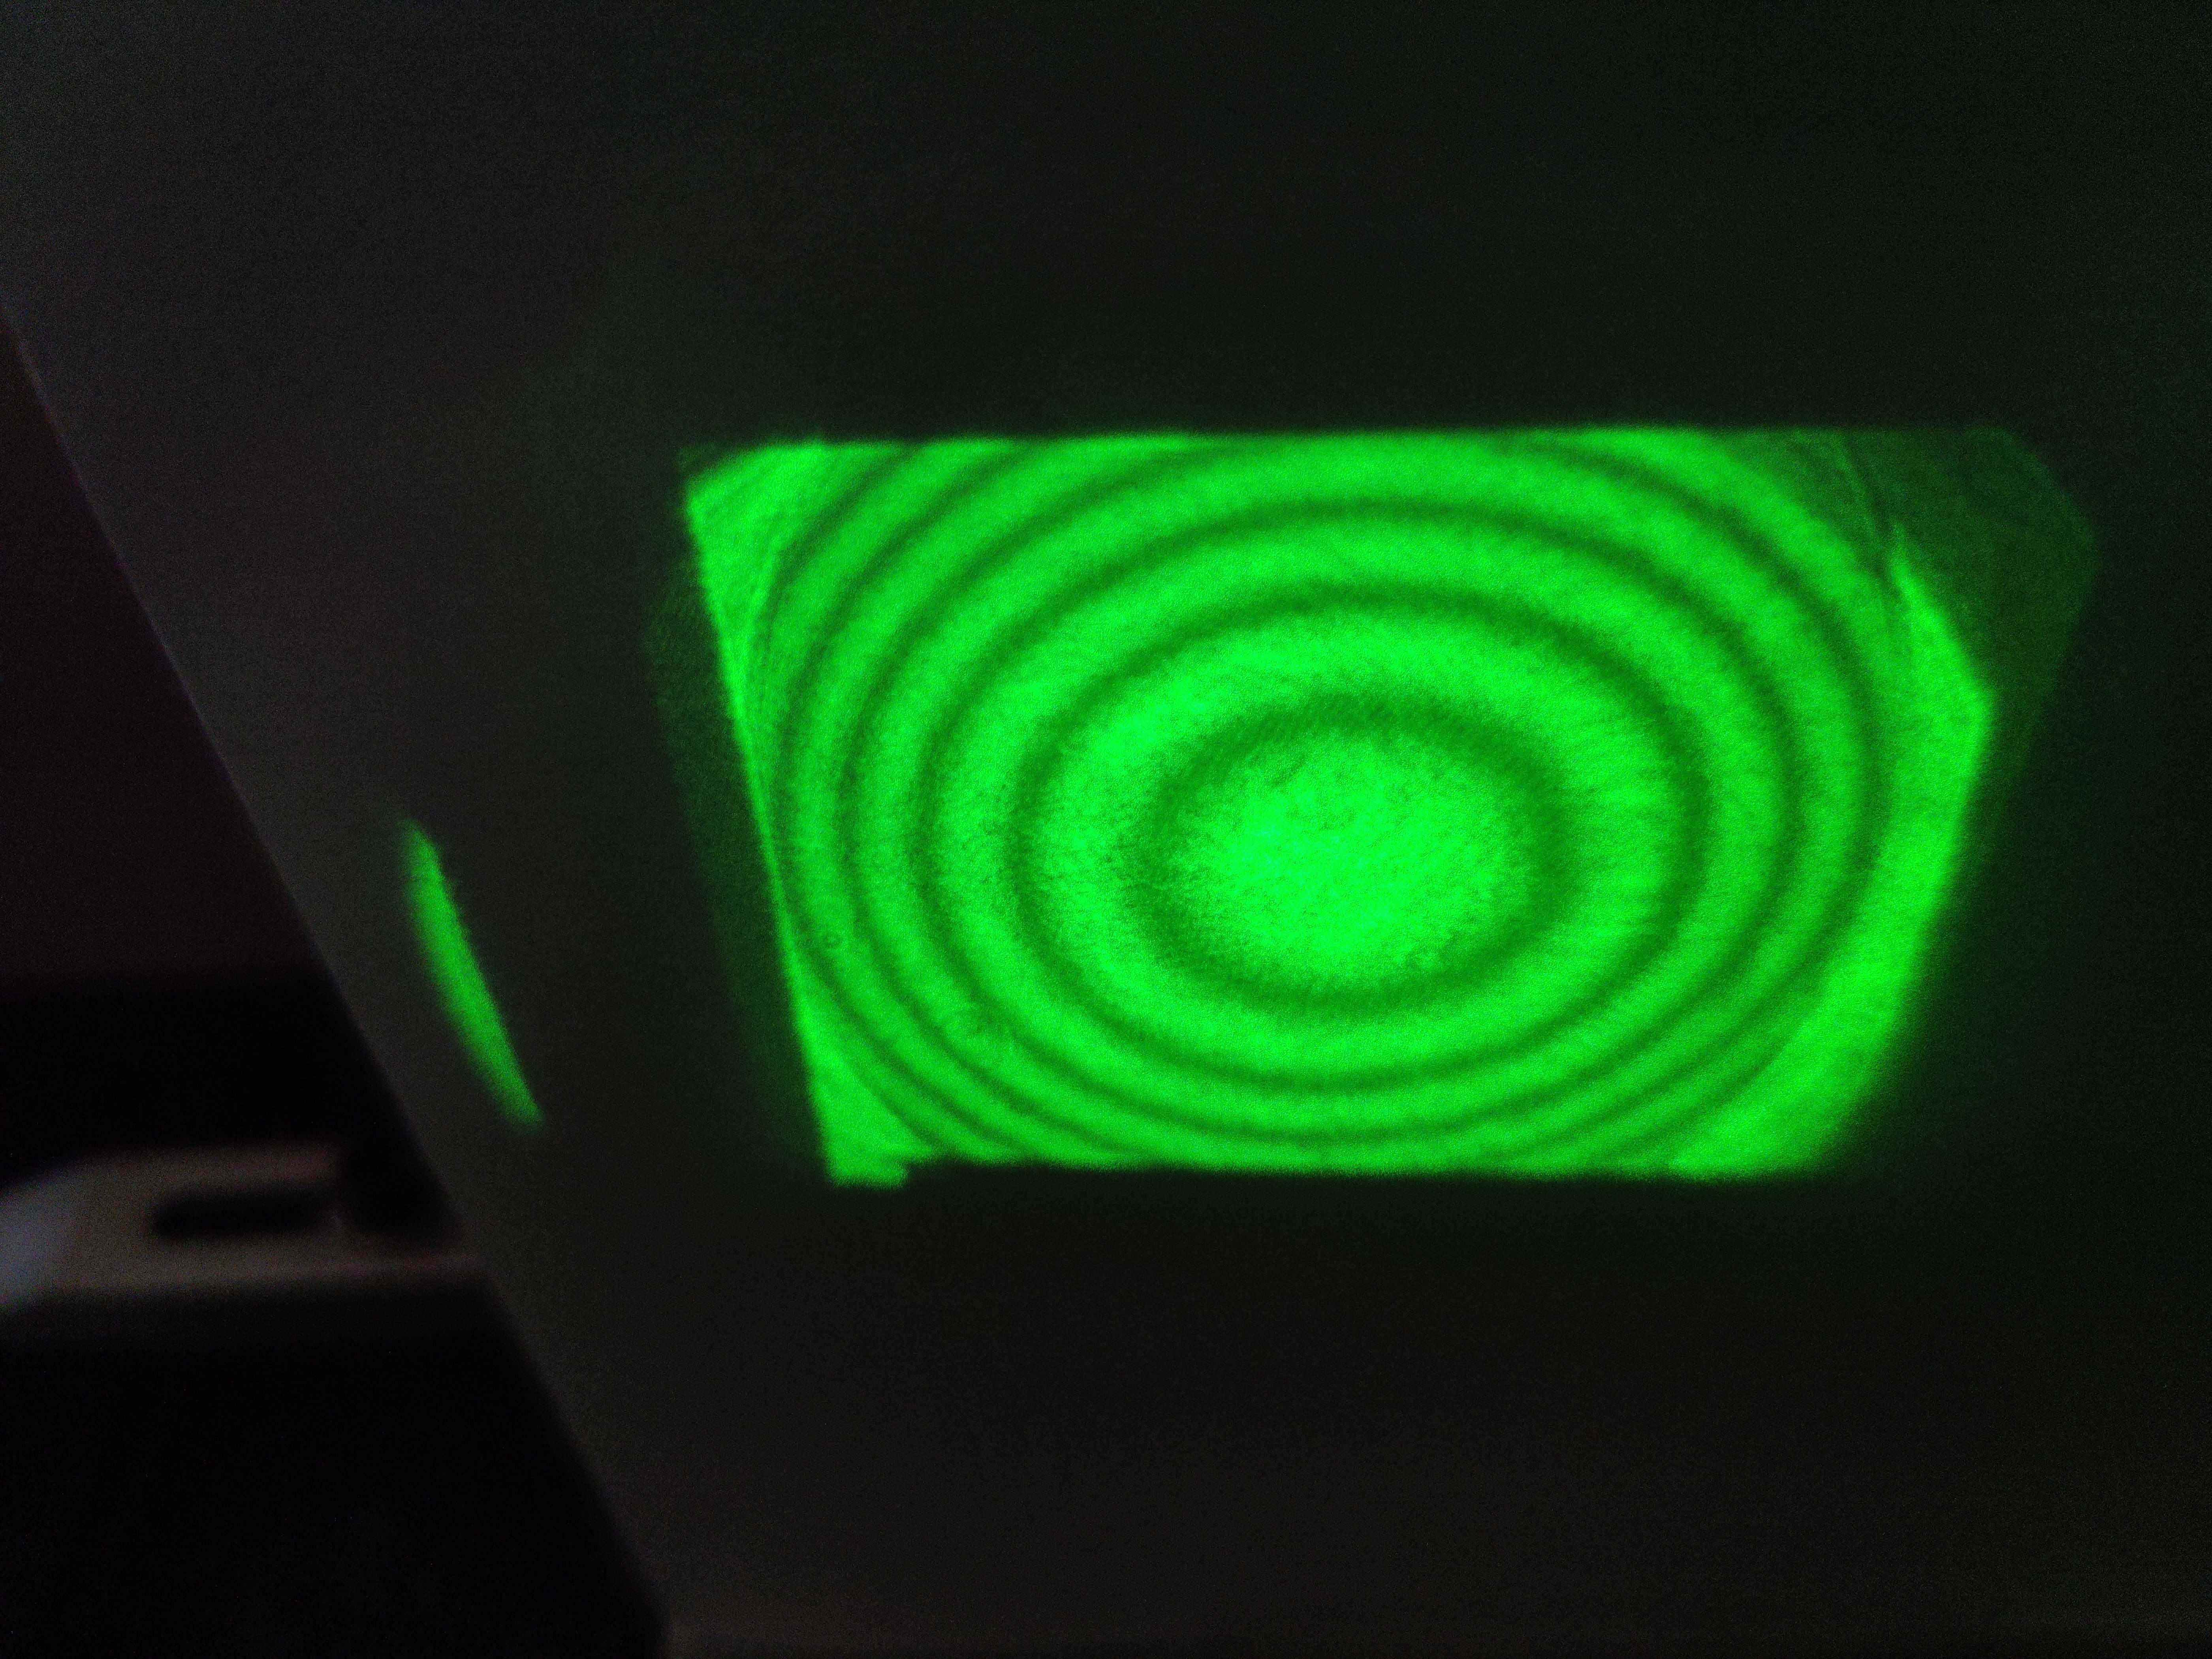
\includegraphics[width=\linewidth]{fig/Compressed/michelson_konz_schirm.jpg}
        \caption{Interferenzmuster des Lasers nach Durchgang durchs Michelsoninterfereometer am Schirm}
        \label{fig:michelson_konz_sammel}
    \end{minipage}%
    \hspace*{\fill}
    \begin{minipage}[t]{0.45\linewidth}
        \centering
        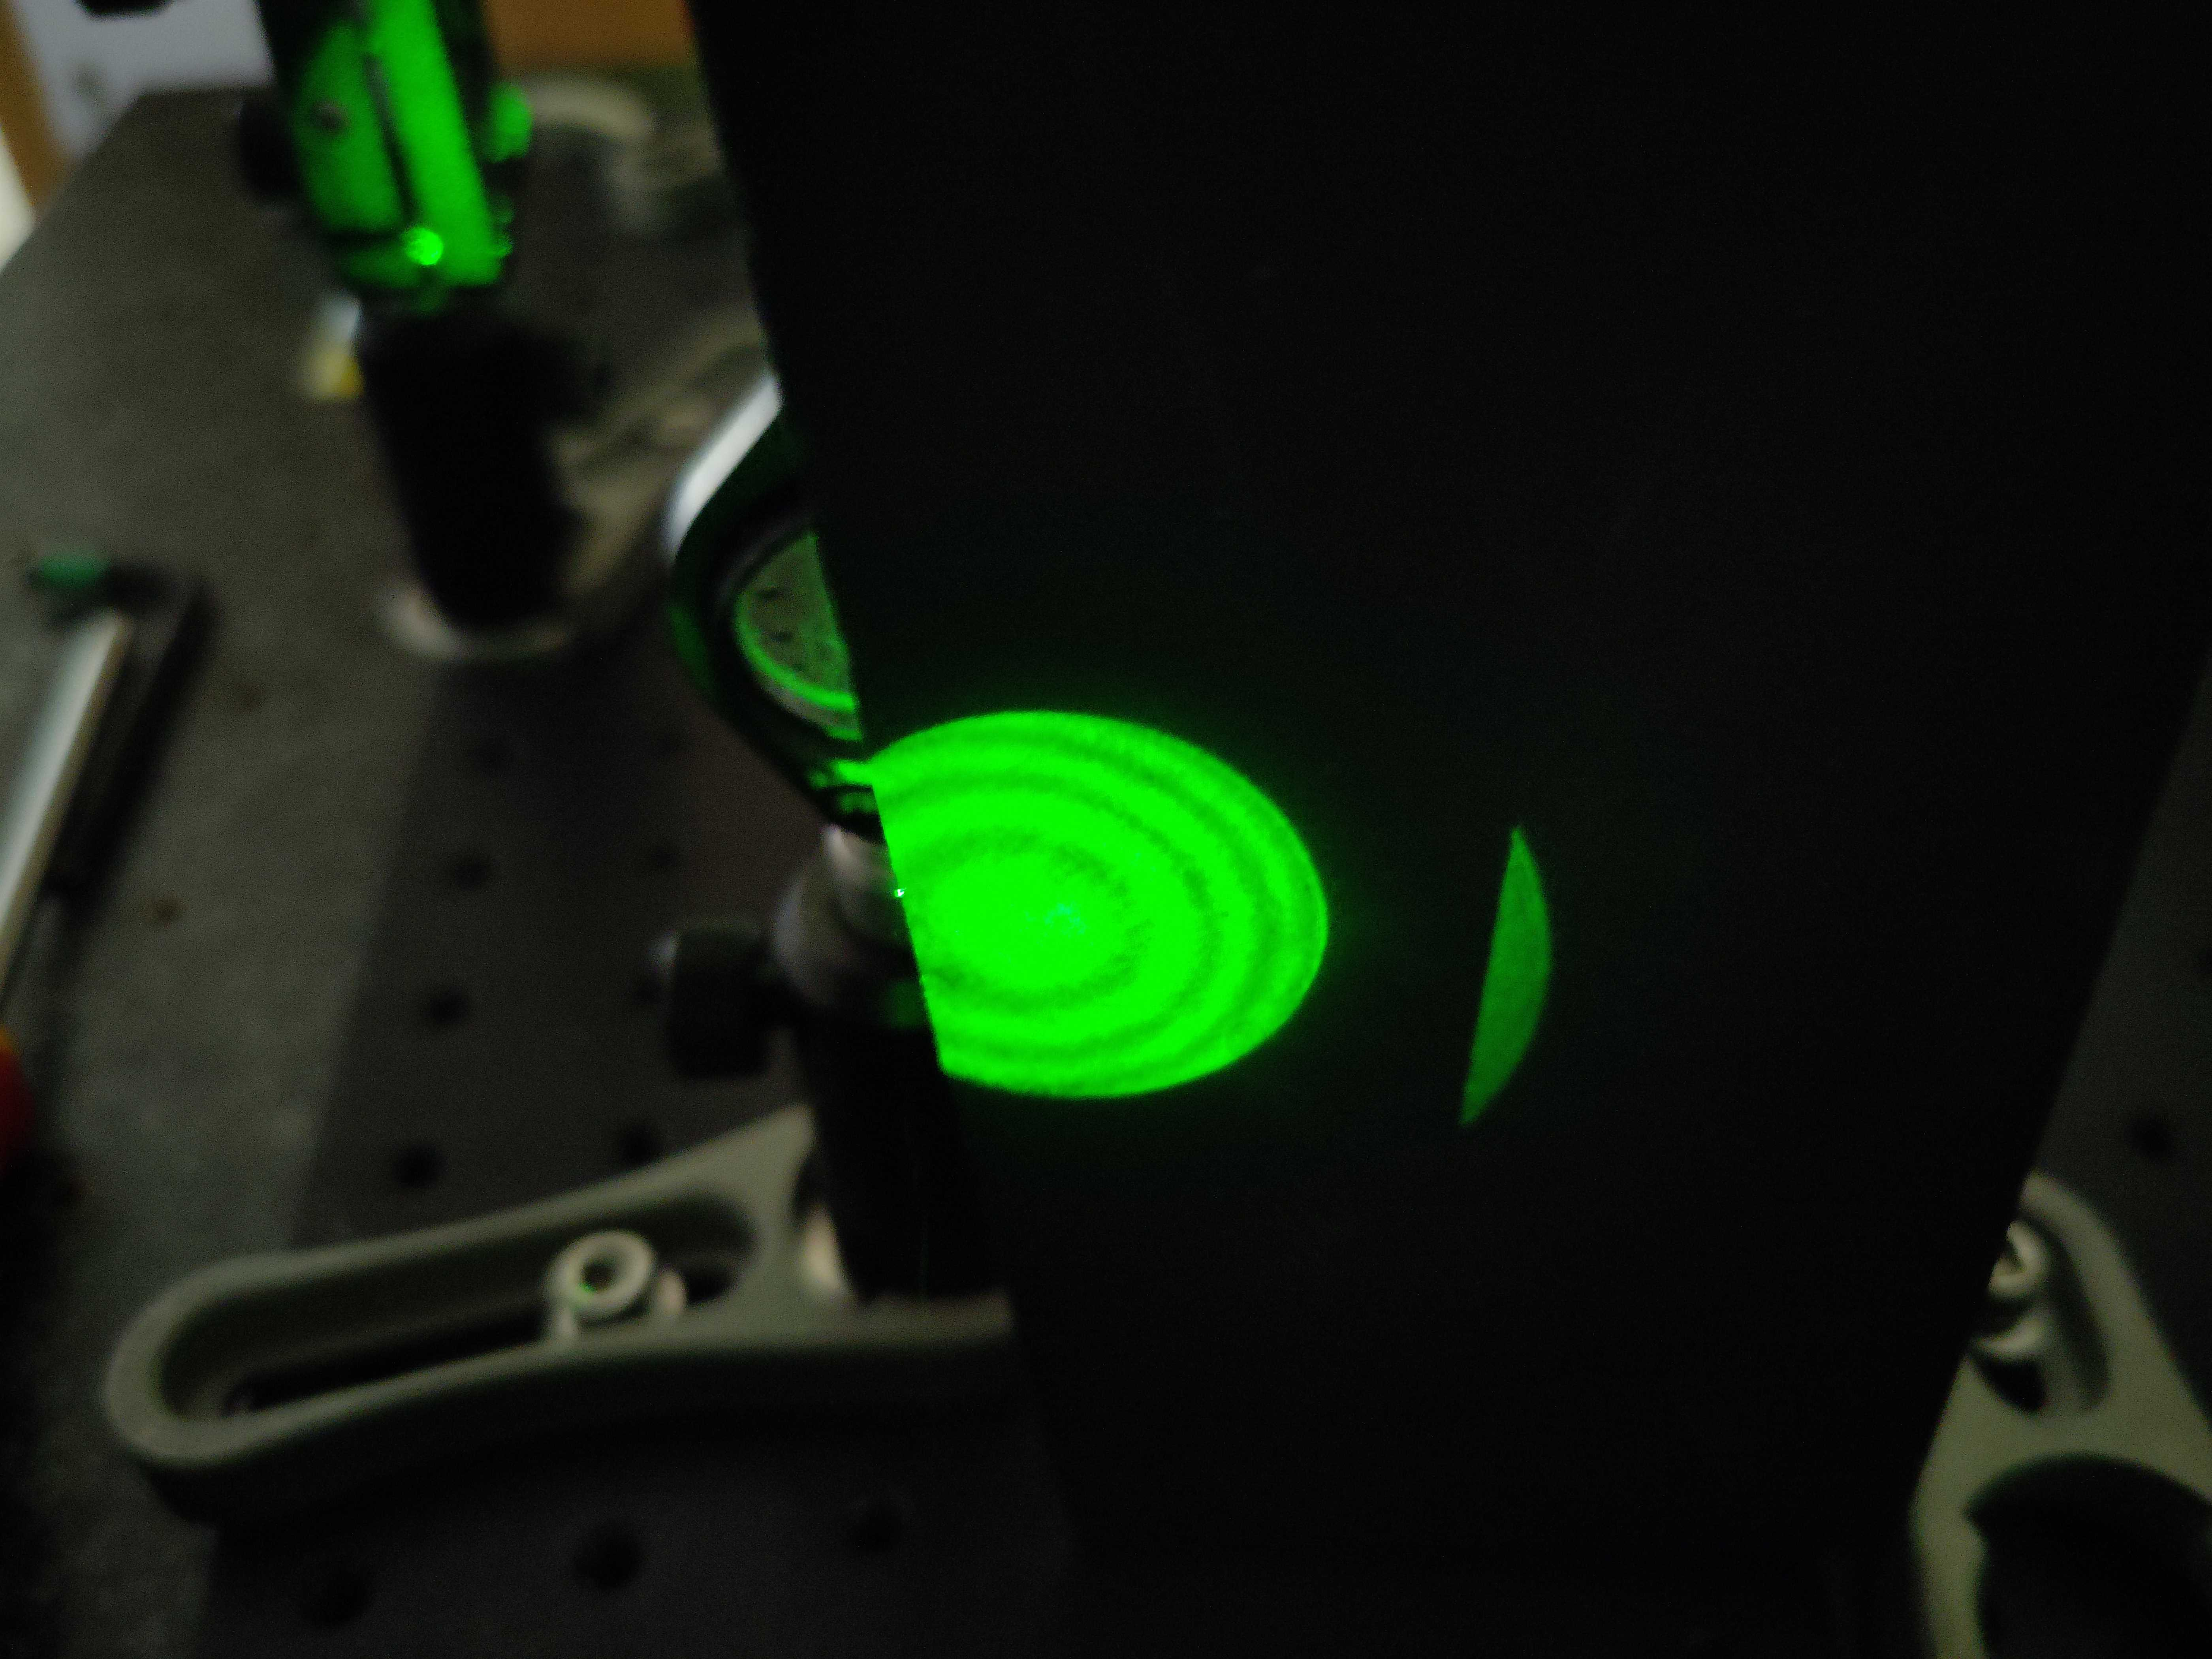
\includegraphics[width=\linewidth]{fig/Compressed/michelson_konz_tuer.jpg}
        \caption{Interferenzmuster des Lasers nach Durchgang durchs Michelsoninterfereometer neben dem Laser}
        \label{fig:michelson_konz_sammel_tuer}
    \end{minipage}
\end{figure}
\setcaphanging

Zur Bestimmung der Wellenlänge des Lasers wird nun mittels Mikrometerschraube ein Spiegel im Michelson-Interfereometer verschoben. Dies führt nun dazu, dass sich das Interferenzmuster am Schirm ändert, da der Gangunterschied zwischen den beiden Teilstrahlen geändert wird. Die Wellenlänge des Lasers kann nun durch die Verschiebung des Spiegels bestimmt werden, indem man die Anzahl der Maxima/Minima beim verschieben um eine gewisse Distanz misst. Konkret wurde so lange an der Mikrometerschraube gedreht, bis am Schirm $n = \num{100(1)}$ neue Maxima/Minima zu sehen waren. Dabei verschiebt sich der Spiegel um eine Distanz von $d_\text{Spiegel-S} = \SI{26.4(10)}{\micro\meter}$, wobei hier schon die Übersetzung der Mikrometerschraube zur tatsächlichen Spiegelbewegung (Faktor \num{5.3}) berücksichtigt wurde. Die Unsicherheit der Mikrometerschraube beläuft sich hier auf $\SI{5}{\micro\meter}$ (nicht untersetzt!). Die Unsicherheit am Start und am Ende der Messung -- um eben möglichst die gleiche Intensität zu erreichen -- wird auf etwa $\SI{0.3}{\micro\meter}$ geschätzt.

Nun wird statt der Sammellinse eine Zerstreuungslinse eingesetzt und die Interferenzmuster erneut beobachtet. Es ergeben sich nun mit der Zerstreuungslinse keine konzentrischen Kreise im Interferzbild, sondern Linien-Interferenzmuster, wie auch in \autoref{fig:michelson_linien_zerstreu} dargestellt.
%info Des is natürlich Bullshit - hab ma vergessen:
Analog zum Versuch mit der eingesetzten Sammellinse werden nun auch 100 Wechsel zwischen Maxima und Minima gezählt. Es ergibt sich für eine Distanz von $d_\text{Spiegel-Z} = \SI{26.6(10)}{\micro\meter}$ für die $n = \num{100(1)}$ Wechsel zwischen Maxima und Minima. Die Unsicherheit dieser Messung wird ebenso analog zum vorherigen versuch mit der konzentrischen Linse angenommen.
\begin{figure}[H]
    \centering
    \begin{samepage}
        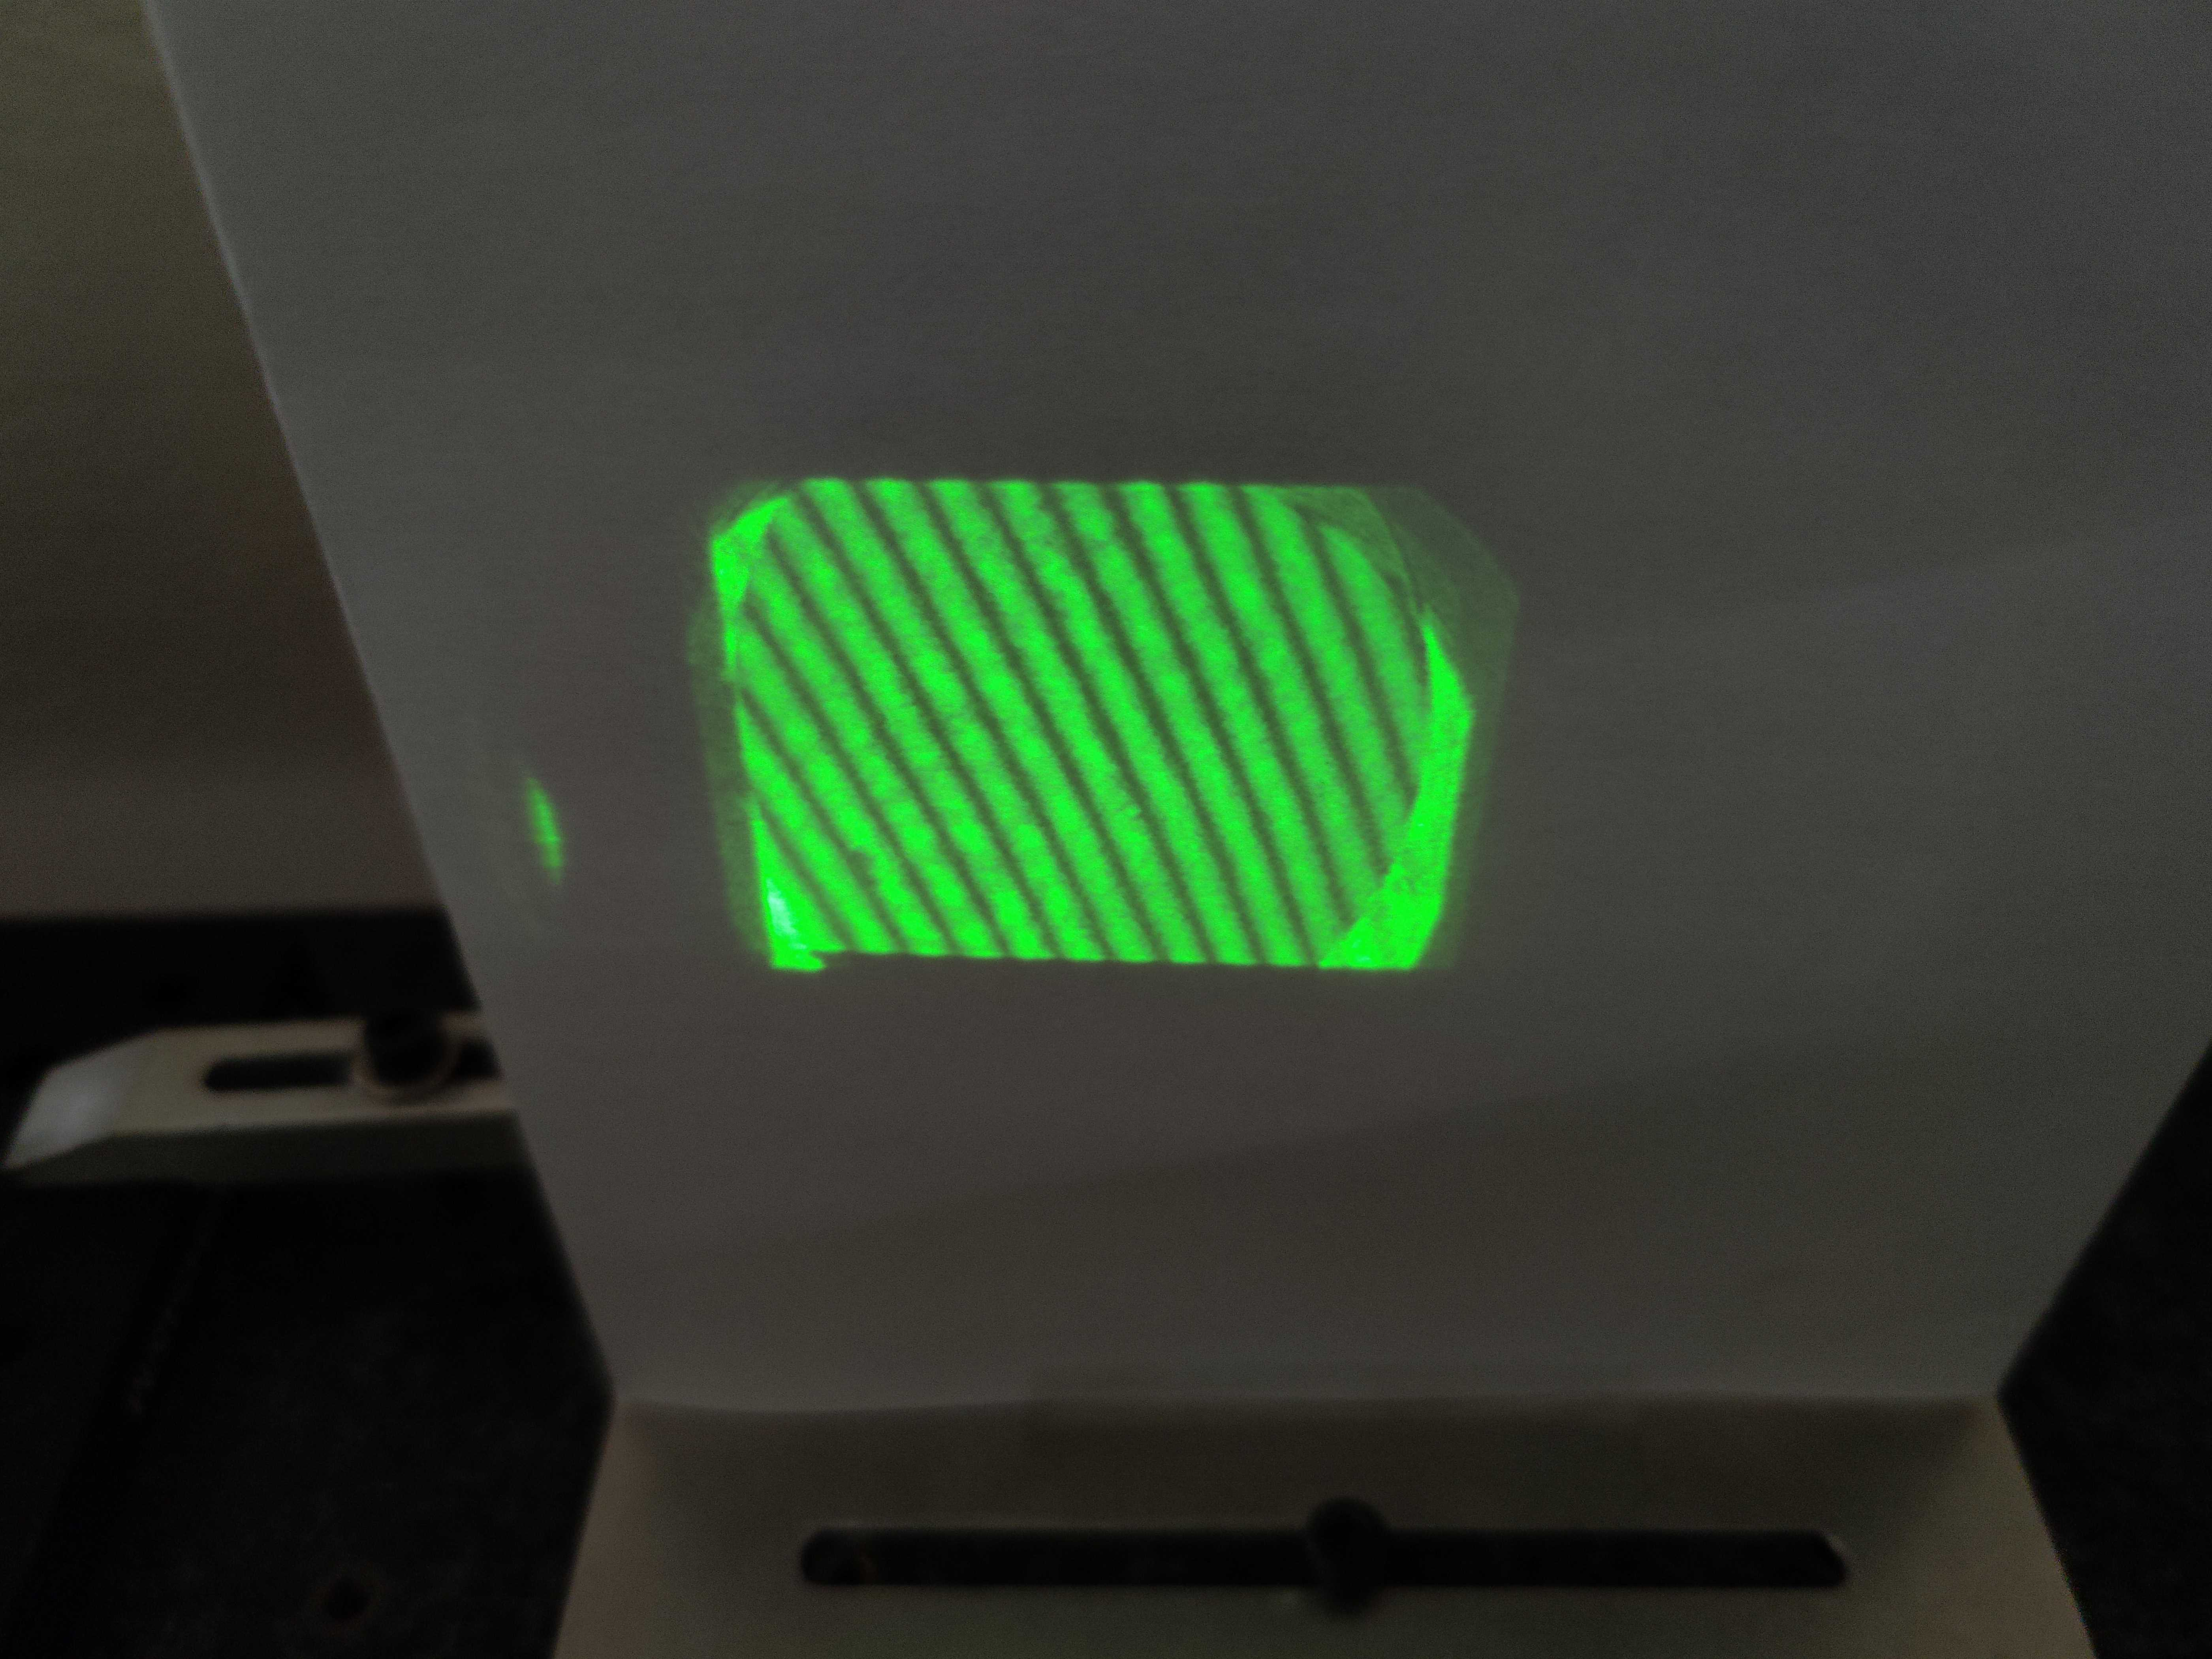
\includegraphics[width=0.7\linewidth]{fig/Compressed/Zerstreuungslinse.jpg}
        \caption{Interferenzmuster des Lasers nach Durchgang durchs Michelsoninterfereometer mit Zerstreuungslinse}
        \label{fig:michelson_linien_zerstreu}
    \end{samepage}
\end{figure}

Nun werden noch externe Änderungen, wie etwa die Auswirkungen der Stellschrauben untersucht. Dabei verstellt eine Schraube die Dichte -- sprich die Anzahl an sichtbaren Maxima/Minima -- und die andere die Ausrichtung, es erfolgt quasi eine Drehung der Maxima/Minima um die Flächennormale.
Die Auswirkungen von Wärmeeinflüssen ist im \underline{\href{https://etschgi1.github.io/files/UNI_hosting/Misc/FP2/Interferometrie/Stoerungen.mp4}{Video}} zu sehen.

Zudem wird noch untersucht, wie sich Polarisationsfilter im Strahlengang des Michelsoninterfereometer auf das Interferenzbild auswirken.
Dazu wird zuerst, wie in \autoref{fig:michelson_pol_vor} ersichtlich, nur ein Filter (\SI{45}{\degree} zur Senkrechten gedreht) vor dem Interferometer platziert. Anschließend wir ein Filter in horizontaler Anordnung in einem der beiden Arme platziert, wie in \autoref{fig:michelson_pol_1_horizontal} dargestellt. In \autoref{fig:michelson_pol_2_horizontal} ist ein Filter in horizontaler Anordnung in beiden Armen zu sehen und in \autoref{fig:michelson_pol_mixed} ein Filter in vertikaler und einer in horizontaler Anordnung pro Arm.
\setcapindent{0pt}
\begin{figure}[H]
    \centering
    \begin{minipage}[t]{0.45\linewidth}
        \centering
        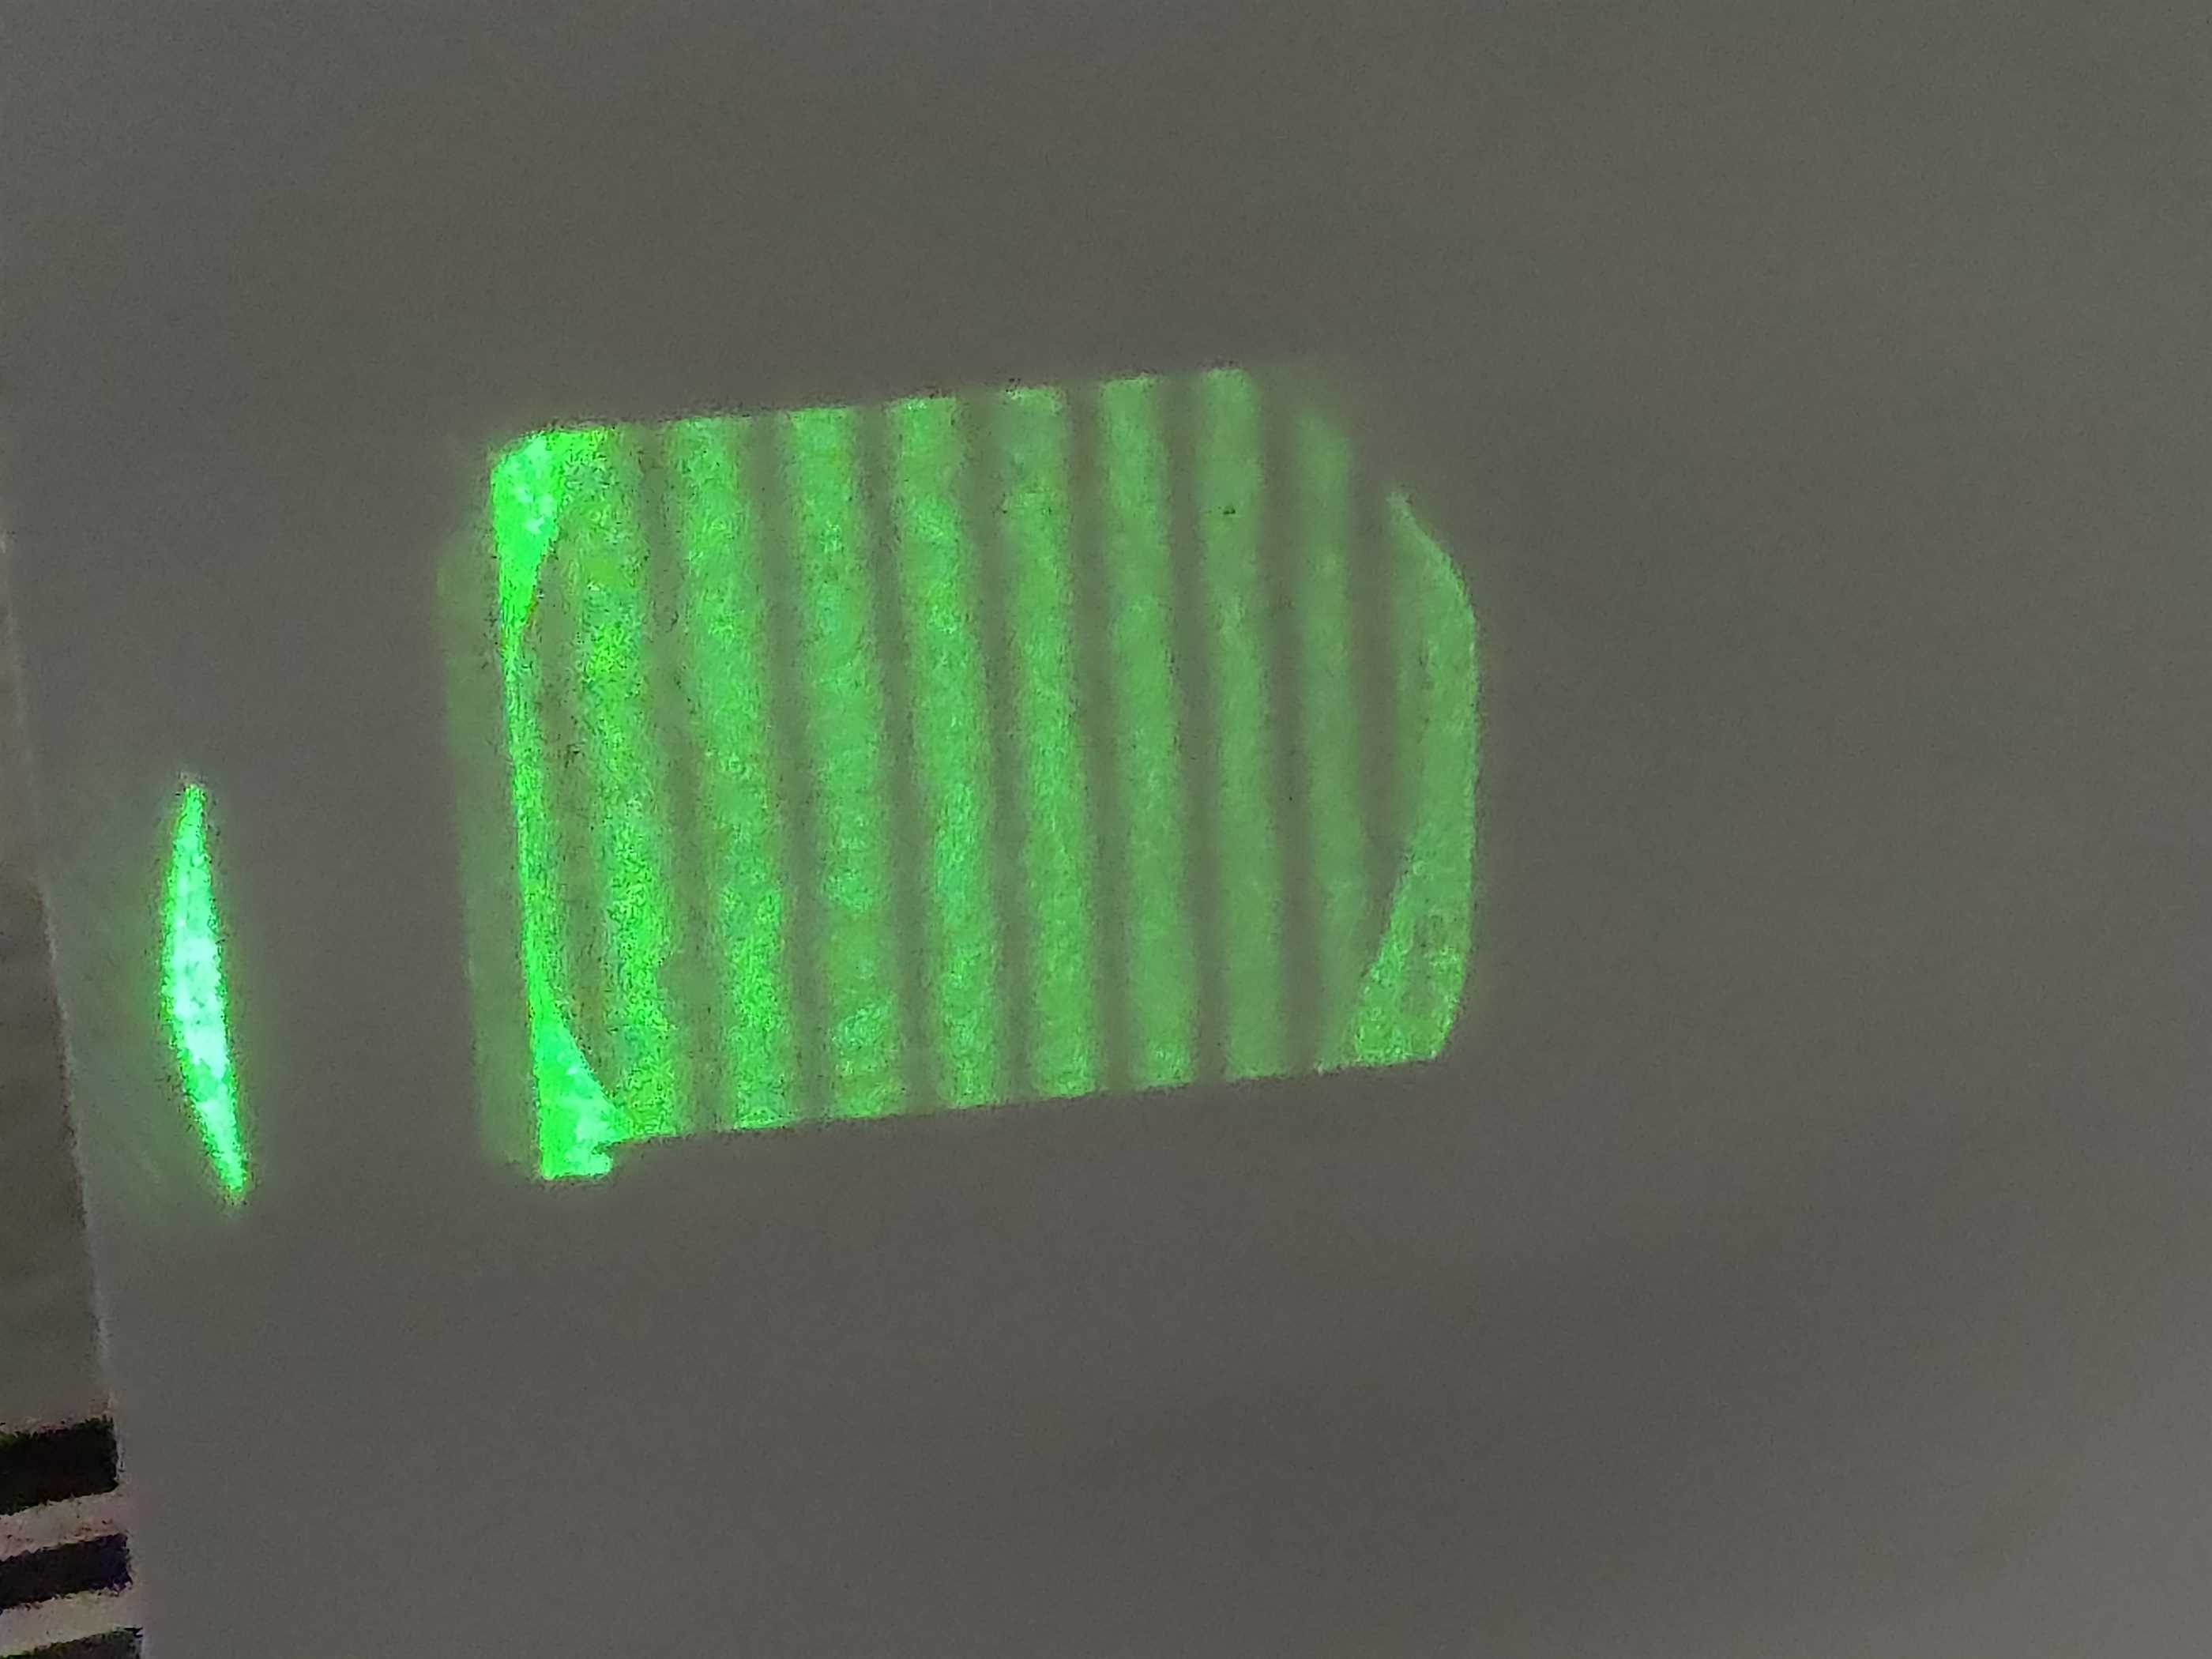
\includegraphics[width=\linewidth]{fig/Compressed/Out_horizontal_detail.jpg} %! is quasi gleich wie nix
        \caption{Interferenzmuster mit einem Polarisator vor dem Interferometer}
        \label{fig:michelson_pol_vor}
    \end{minipage}%
    \hspace*{\fill}
    \begin{minipage}[t]{0.45\linewidth}
        \centering
        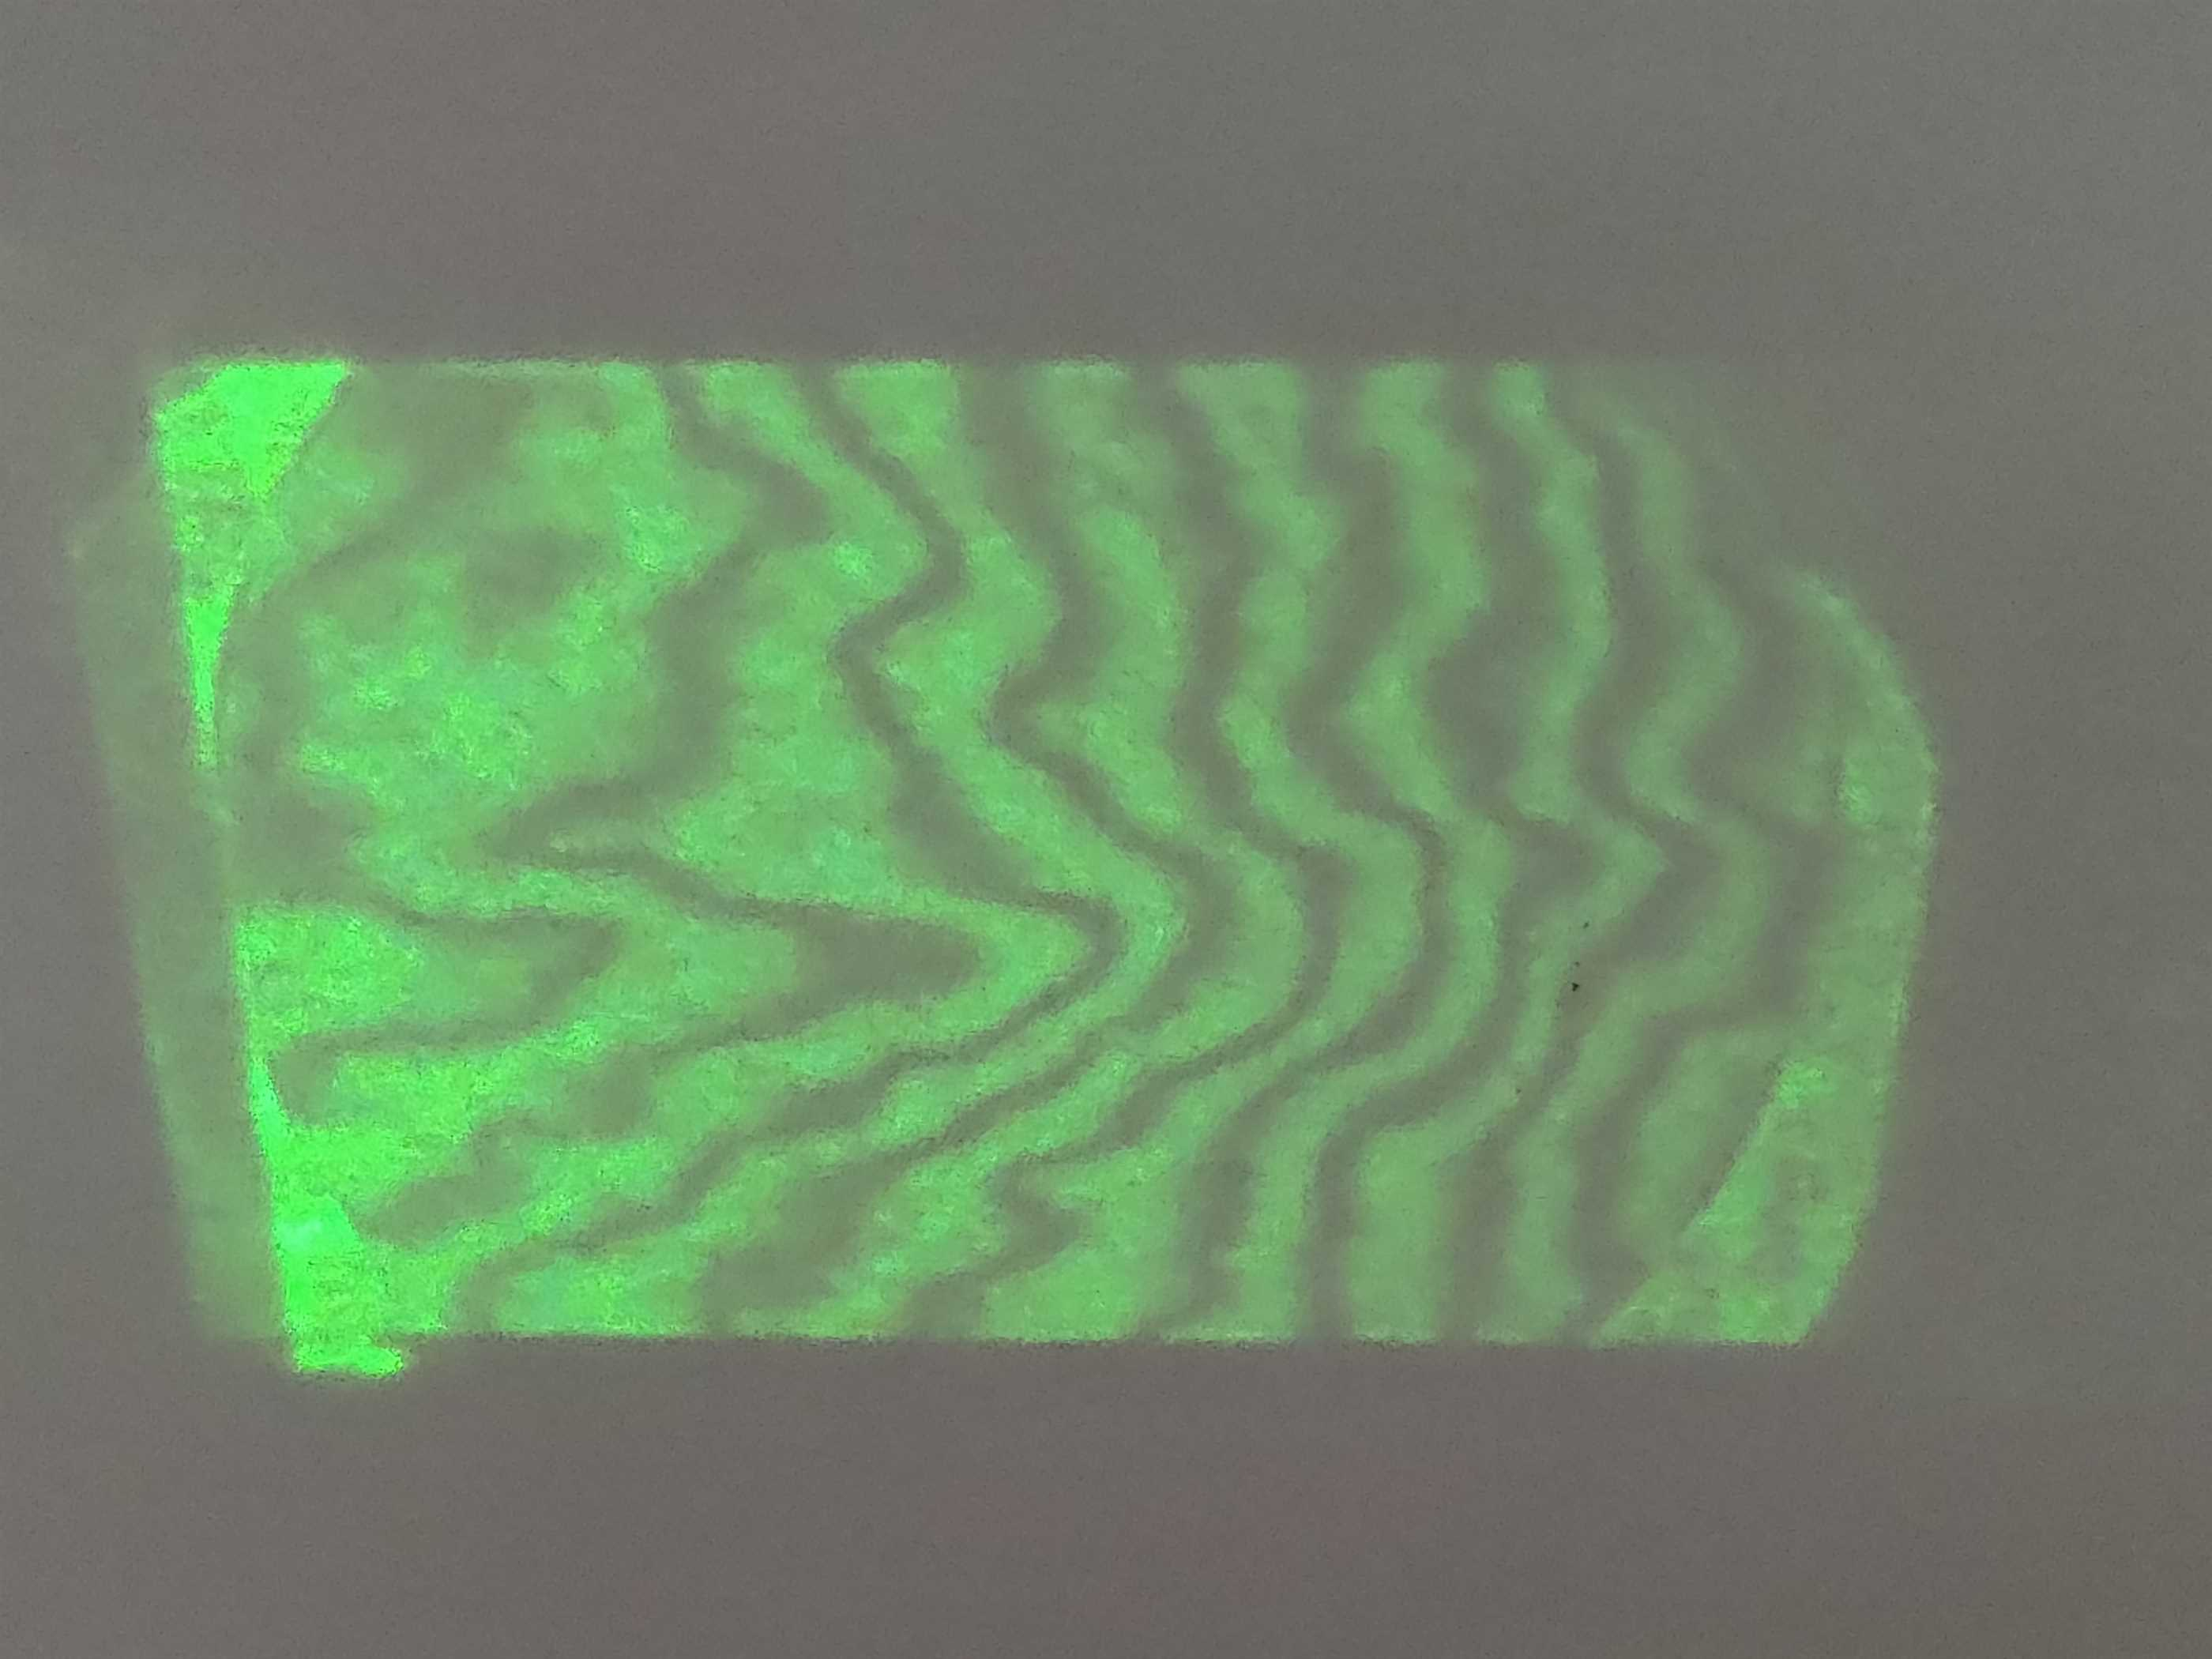
\includegraphics[width=\linewidth]{fig/Compressed/Arago_horizontal_detail.jpg}
        \caption{Interferenzmuster mit einem Polarisator in horizontaler Anordnung in einem Arm}
        \label{fig:michelson_pol_1_horizontal}
    \end{minipage}
\end{figure}
\setcaphanging

\setcapindent{0pt}
\begin{figure}[H]
    \centering
    \begin{minipage}[t]{0.45\linewidth}
        \centering
        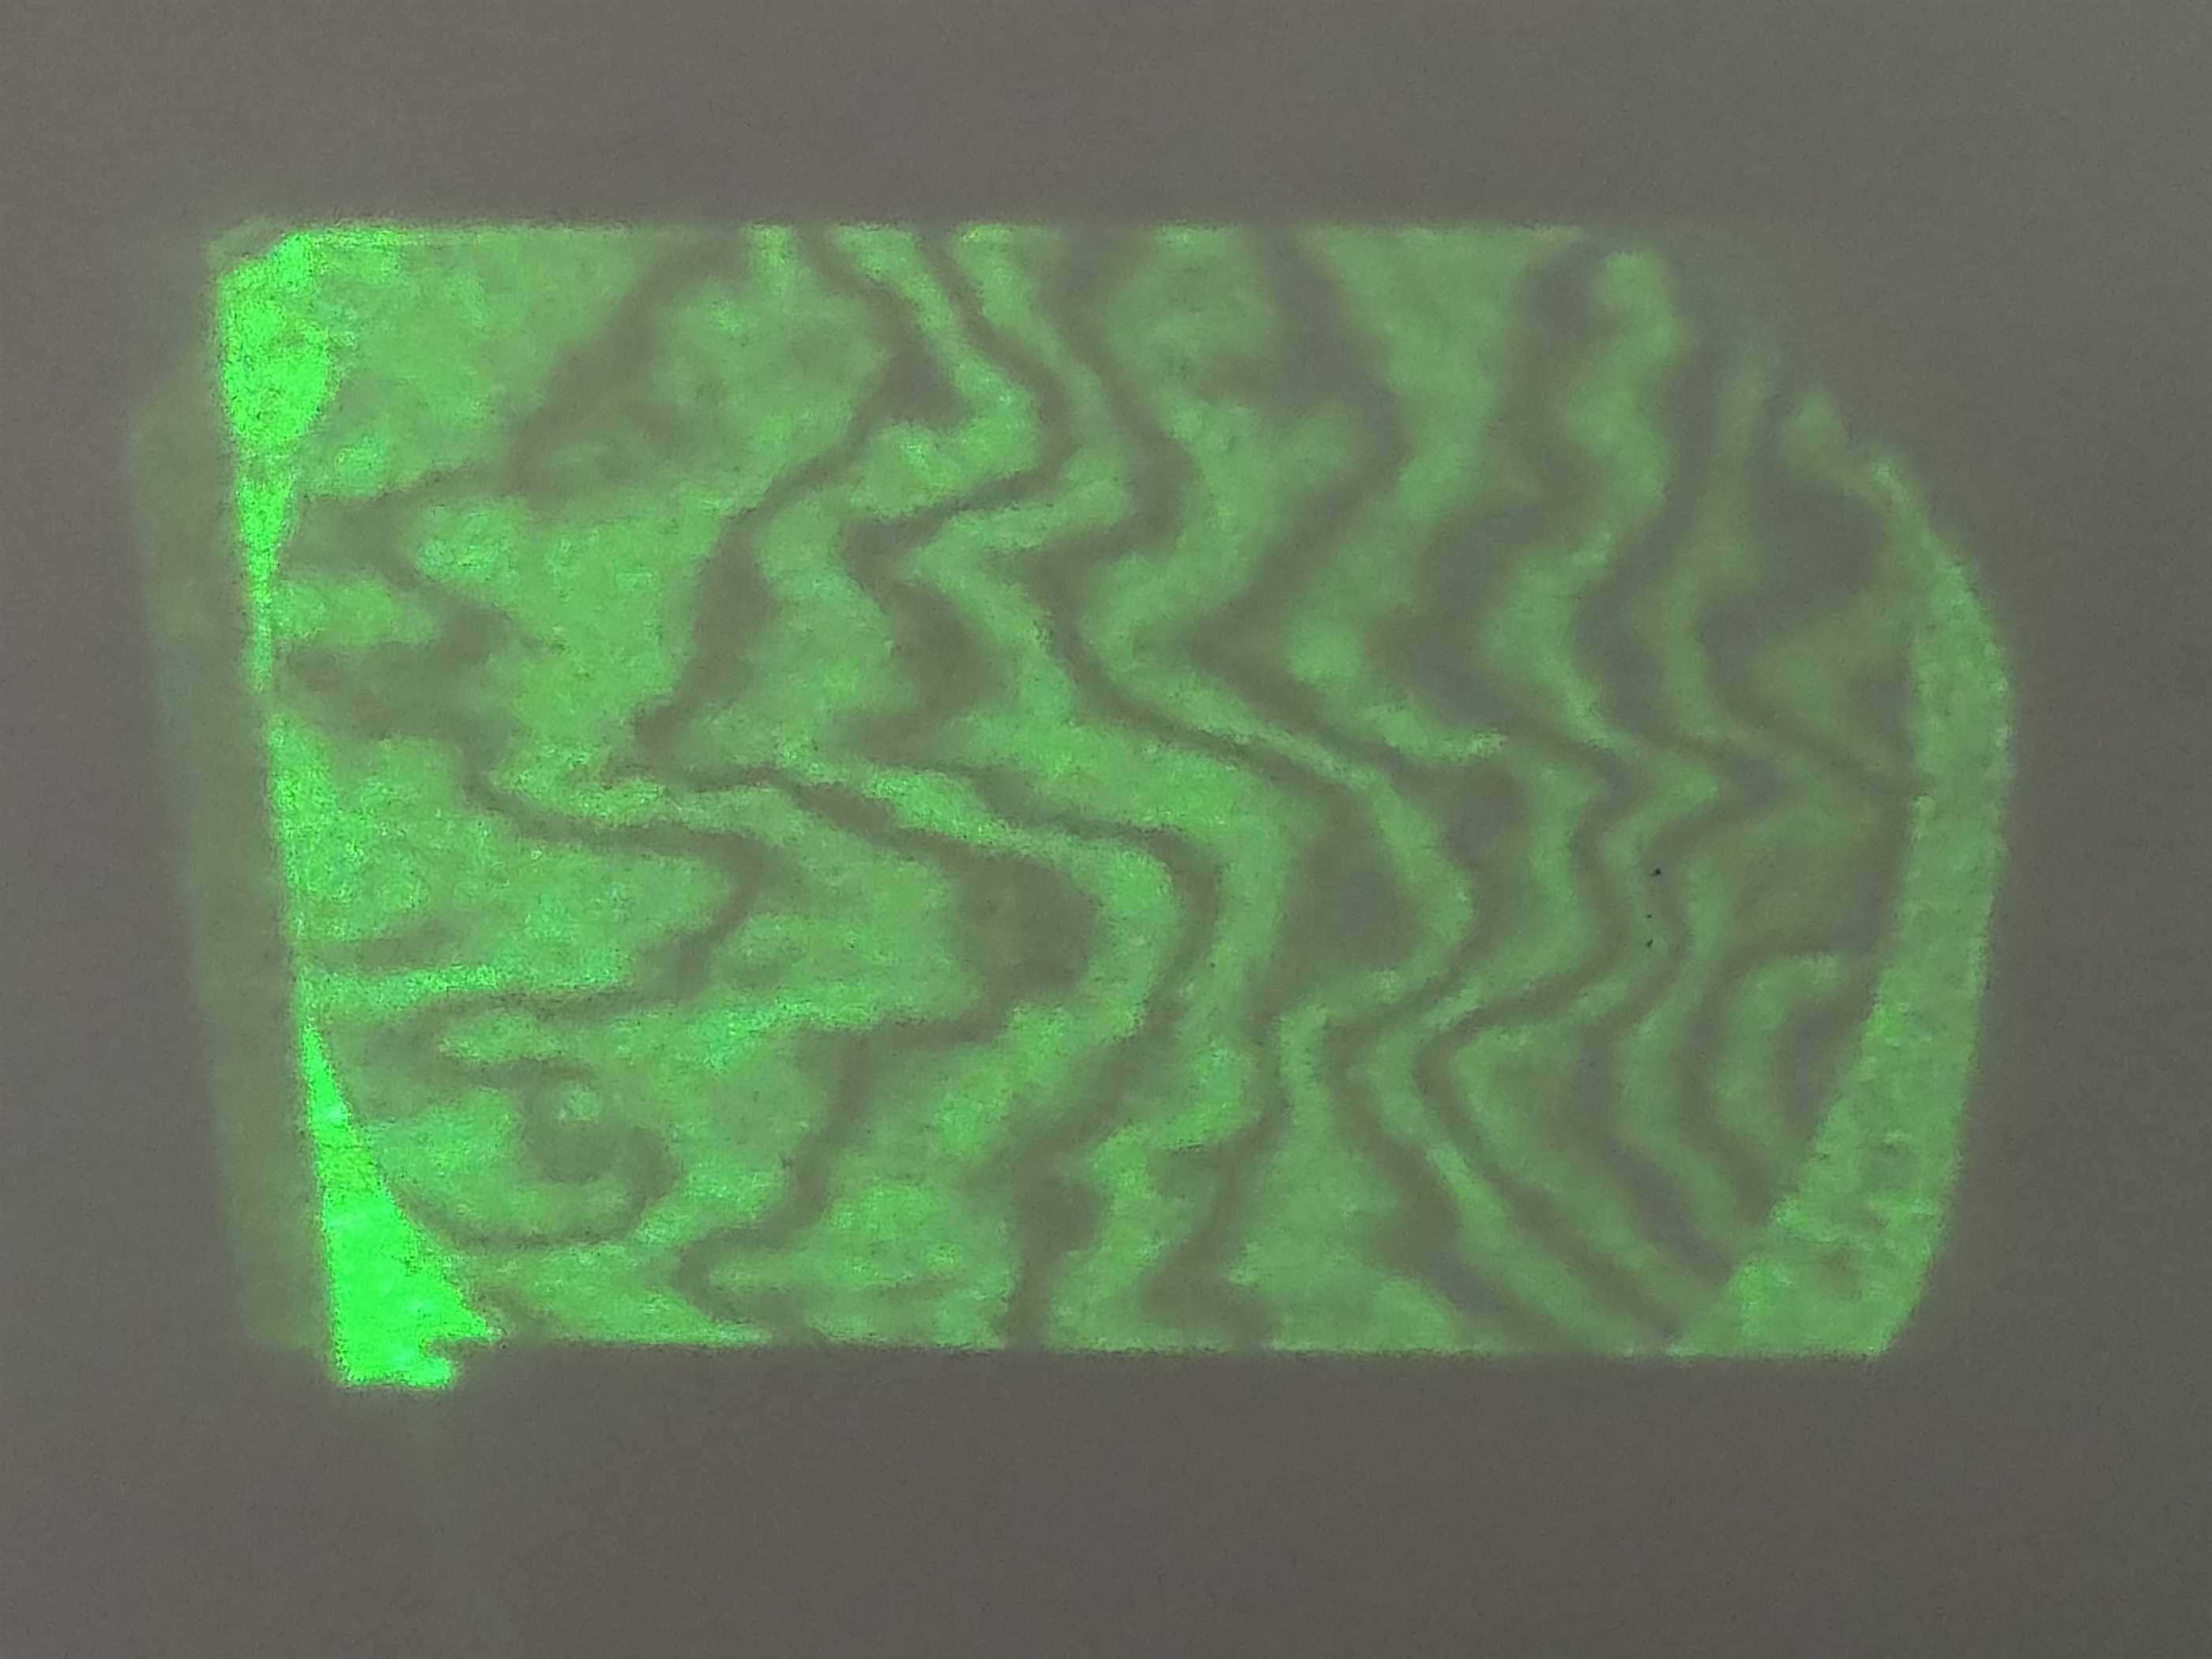
\includegraphics[width=\linewidth]{fig/Compressed/Arago_2_Horizontal_detail.jpg}
        \caption{Interferenzmuster mit jeweils einem Polarisator in horizontaler Anordnung pro Arm}
        \label{fig:michelson_pol_2_horizontal}
    \end{minipage}%
    \hspace*{\fill}
    \begin{minipage}[t]{0.45\linewidth}
        \centering
        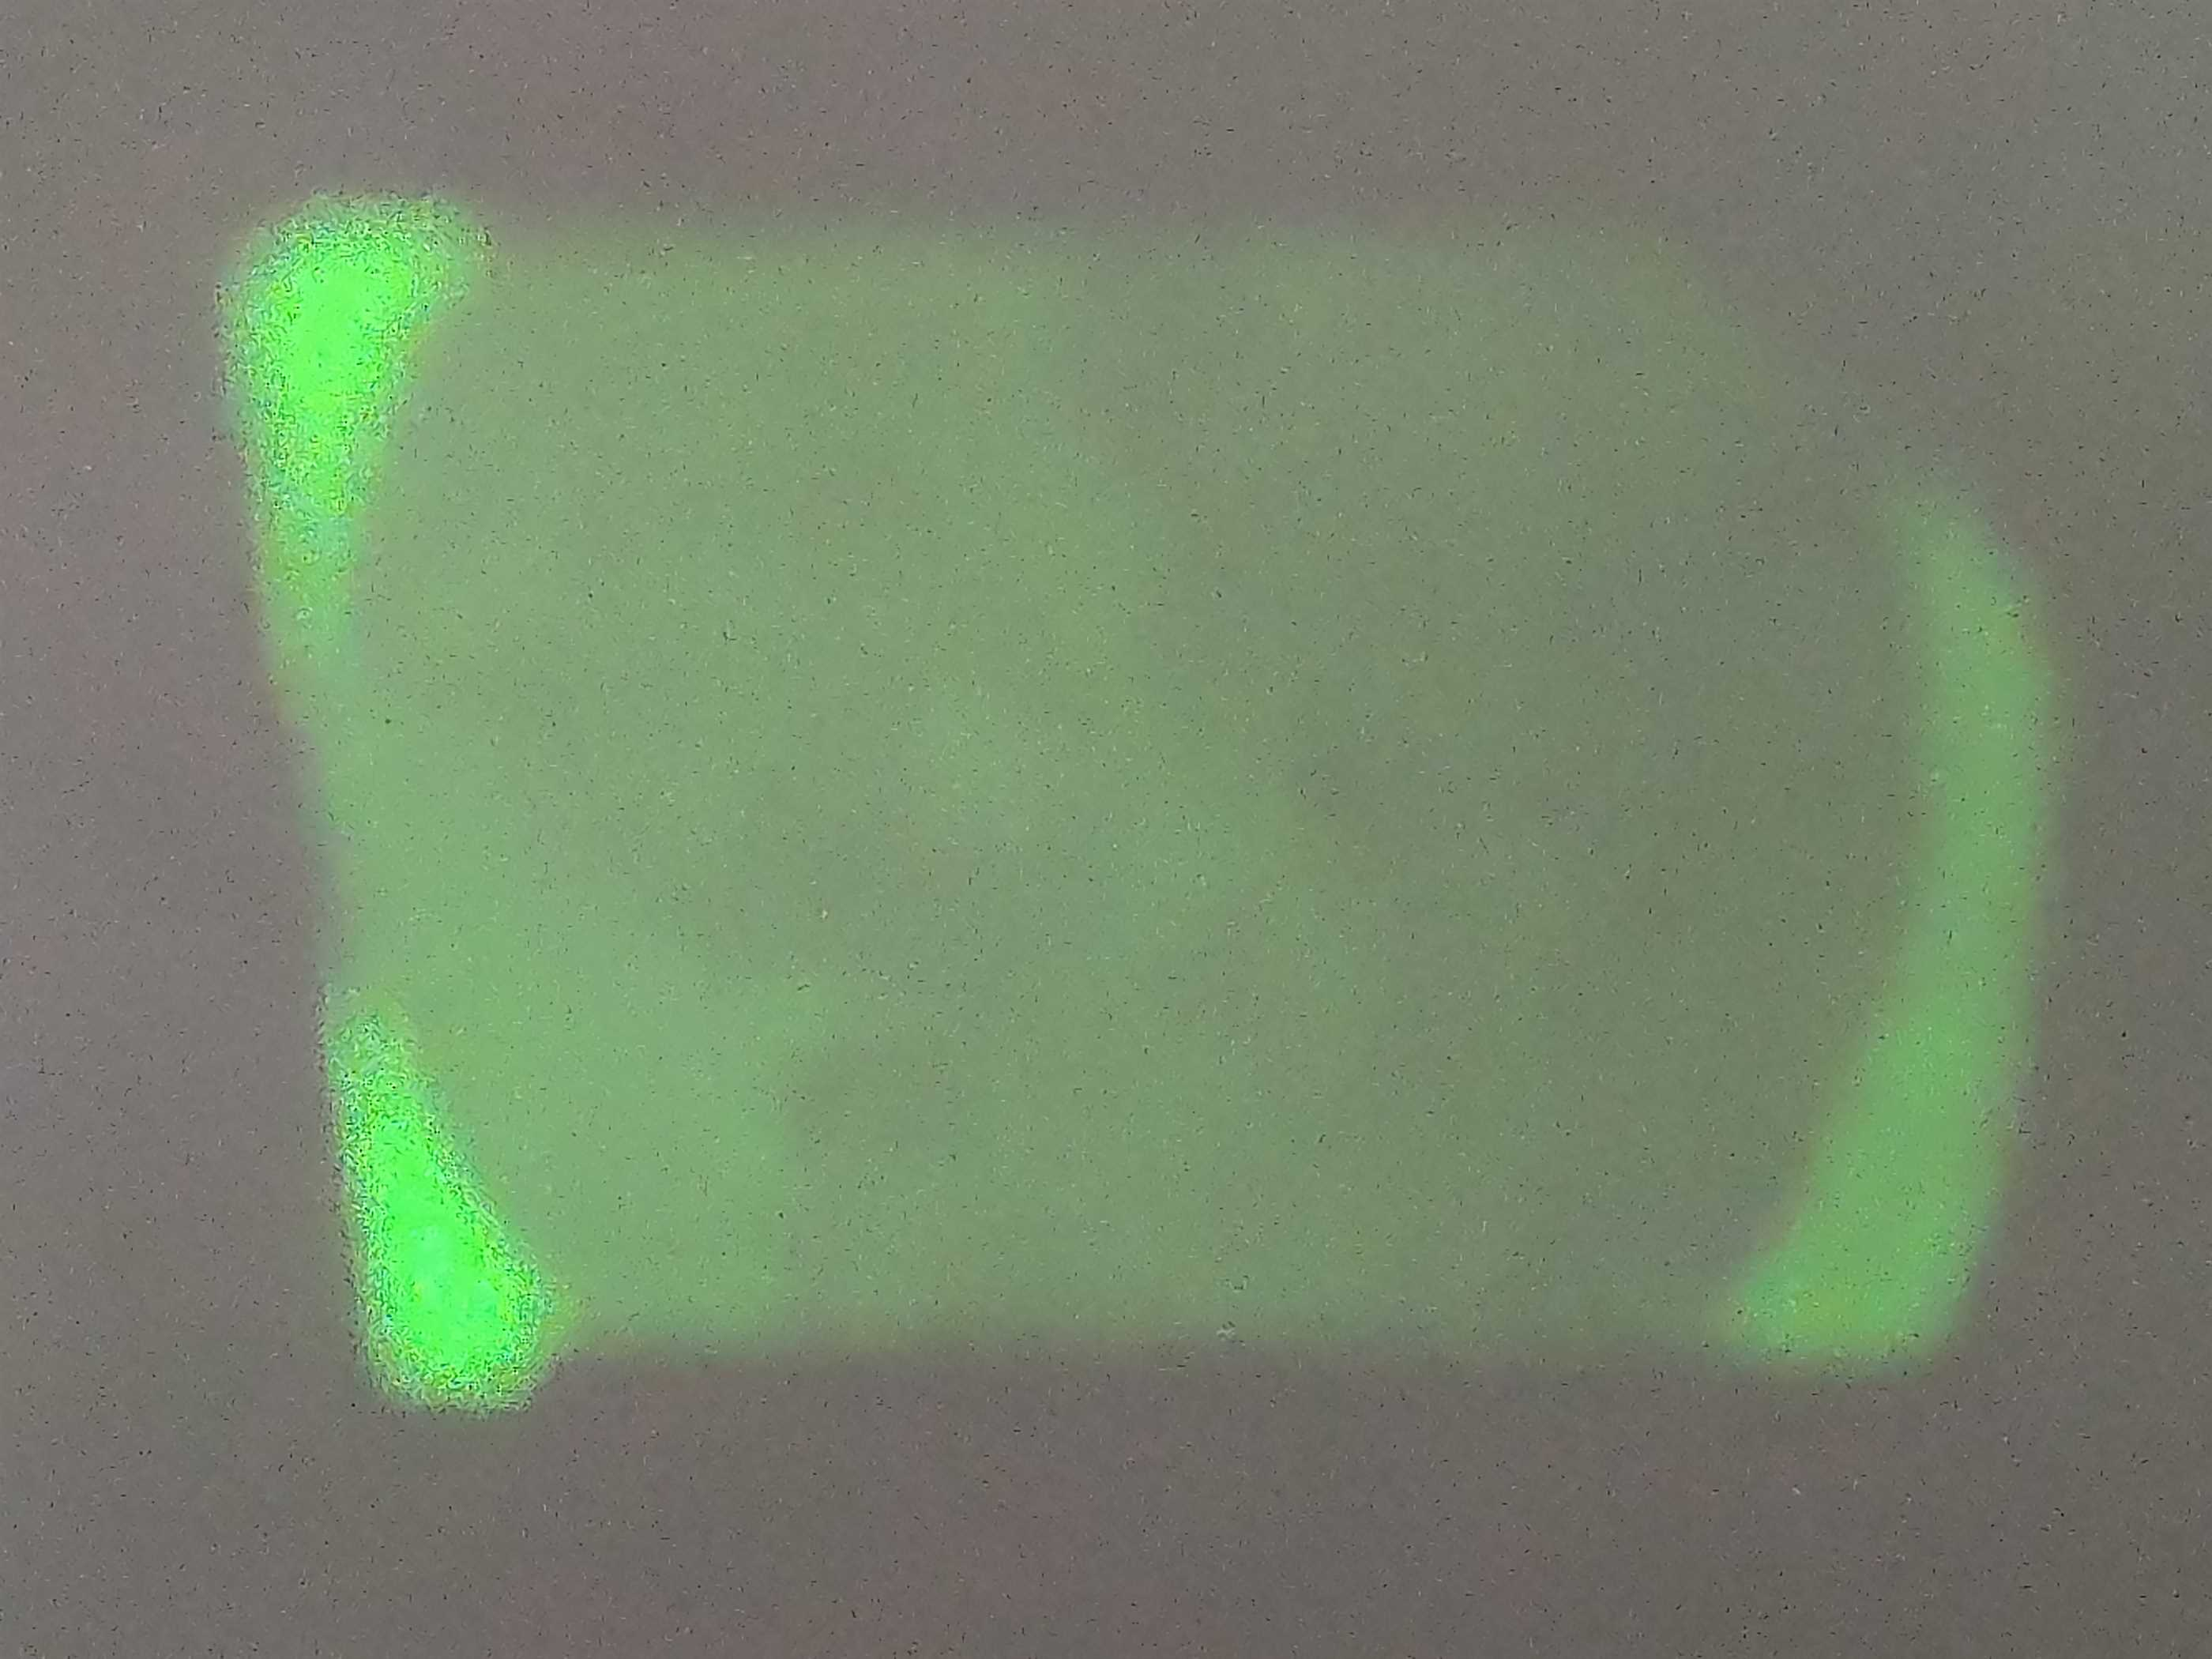
\includegraphics[width=\linewidth]{fig/Compressed/Arago_mixed Detail.jpg}
        \caption{Interferenzmuster mit einem Polarisator in horizontaler Anordnung im ersten Arm und einem mit vertikaler im zweiten Arm}
        \label{fig:michelson_pol_mixed}
    \end{minipage}
\end{figure}
\setcaphanging
%! maybe noch was anderes hier aber sollte sonst gach eh mal passen. 



\section{Auswertung}
\label{sec:auswertung}

\subsection{Young'scher Doppelspalt}
\label{subsec:auswertung_doppelspalt}

Aus den aufgenommenen Interferenzmuster der vier Young'schen Doppelspalte aus den Abbildungen \ref{fig:DS_1_interferenzmuster} bis \ref{fig:DS_4_interferenzmuster} können Intensitätskurven gewonnen werden. Dafür wird zuerst ein Bereich von Interesse ausgeschnitten und zusätzliche mit einem Graufilter belegt, sodass die Intensitätsunterschiede zulasten der Farbdarstellung besser ersichtlich werden. Dies erfolgt mit der Bildbearbeitungssoftware \textit{paint.net}. Aus diesen bearbeiteten Bildern werden mithilfe der Software \textit{ImageJ} Intensitätskurven extrahiert. Da die einzelnen Intensitätsmaxima auch direkt im Labor mit einem Lineal gemessen worden sind, ist die Umrechnung von Pixelpositionen in reale relative Abstände ein leichtes. Hierfür wird pro Doppelspaltintensitätskurve je das 0. und 1. Maximum herangezogen, wobei das 0. Maximum als Koordinatenursprung gewählt wird. Die extrahierten Intensitätskurven sowie die theoretischen Verläufe (Produkt aus Intensität für Beugung und Interferenz, \autoref{eq:intensity_gesamt}) aufgrund der Abmessungen des jeweiligen Doppelspalts werden gegen relative Abstände zum 0. Maximum aufgetragen und sind in den Abbildungen \ref{fig:intensitaet_DS_1} bis \ref{fig:intensitaet_DS_4} ersichtlich. Die mit dem Lineal gemessenen Position der Maxima sind zusätzlich mit einem vertikalen Balken inklusive Unsicherheitsband eingezeichnet.
%
\begin{figure}[H]
    \centering
    \begin{samepage}
        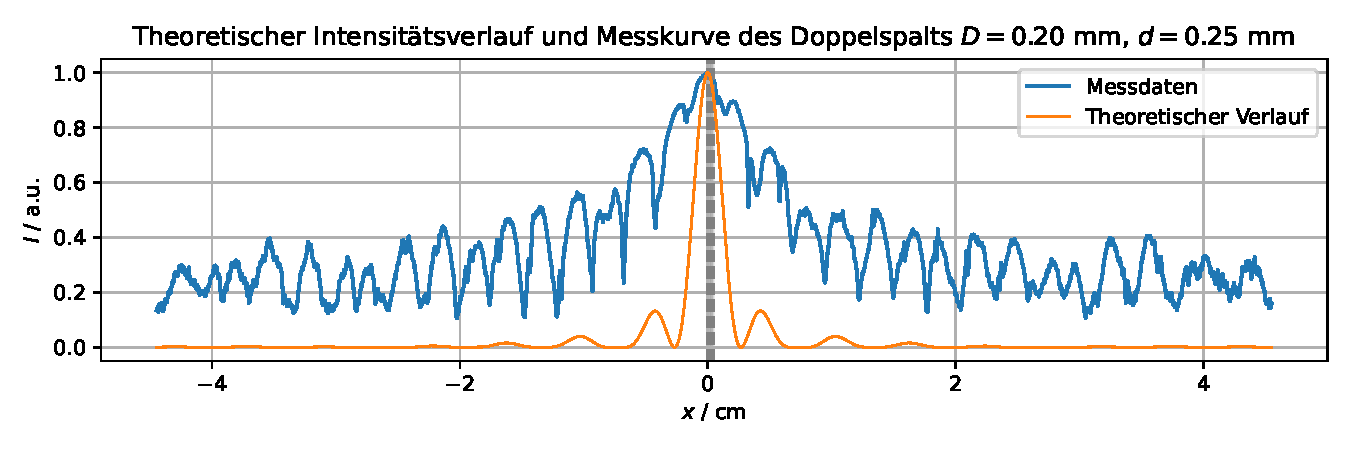
\includegraphics[width=\linewidth]{../python/plots/young_1.pdf}
        \caption[Intensitätskurve DS 1]{Gemessener und theoretischer Intensitätsverlauf des Doppelspalts 1, Messkurve aus \autoref{fig:DS_1_interferenzmuster} extrahiert.}
        \label{fig:intensitaet_DS_1}
    \end{samepage}
\end{figure}
\begin{figure}[H]
    \centering
    \begin{samepage}
        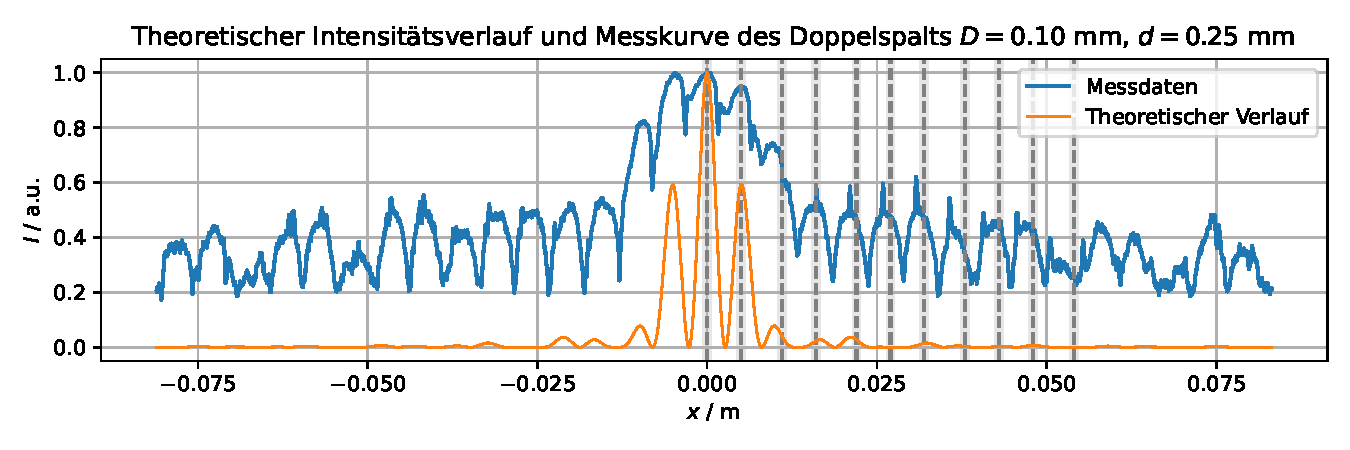
\includegraphics[width=\linewidth]{../python/plots/young_2.pdf}
        \caption[Intensitätskurve DS 2]{Gemessener und theoretischer Intensitätsverlauf des Doppelspalts 2, Messkurve aus \autoref{fig:DS_2_interferenzmuster} extrahiert.}
        \label{fig:intensitaet_DS_2}
    \end{samepage}
\end{figure}
\begin{figure}[H]
    \centering
    \begin{samepage}
        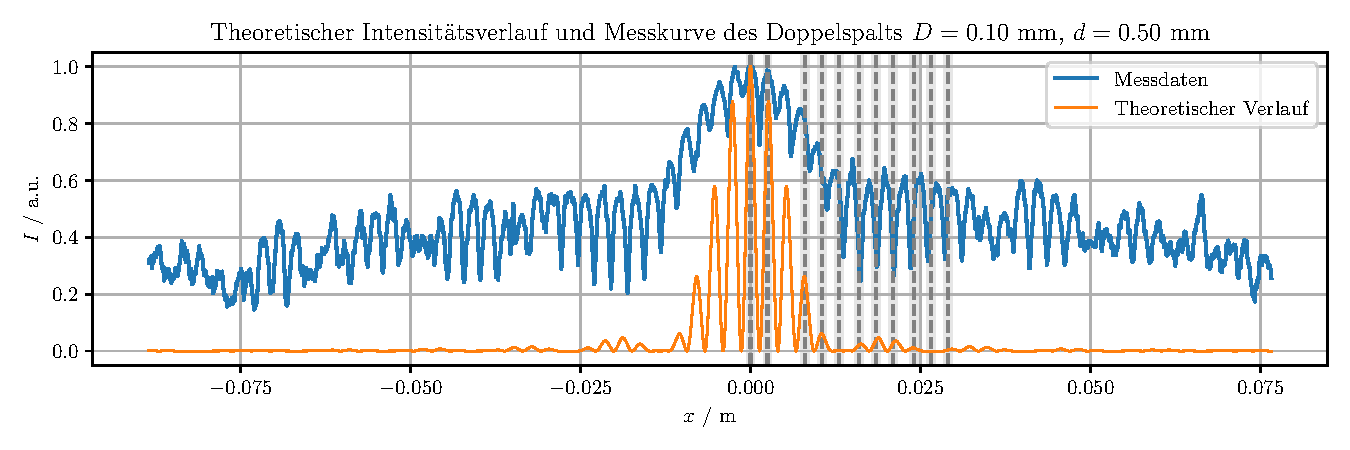
\includegraphics[width=\linewidth]{../python/plots/young_3.pdf}
        \caption[Intensitätskurve DS 3]{Gemessener und theoretischer Intensitätsverlauf des Doppelspalts 3, Messkurve aus \autoref{fig:DS_3_interferenzmuster} extrahiert.}
        \label{fig:intensitaet_DS_3}
    \end{samepage}
\end{figure}
\begin{figure}[H]
    \centering
    \begin{samepage}
        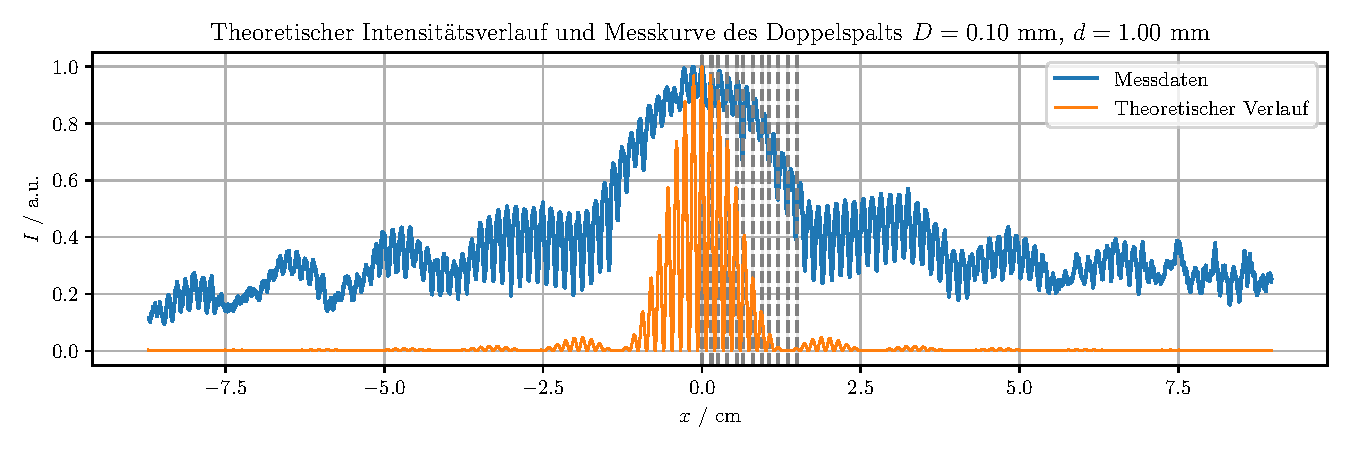
\includegraphics[width=\linewidth]{../python/plots/young_4.pdf}
        \caption[Intensitätskurve DS 4]{Gemessener und theoretischer Intensitätsverlauf des Doppelspalts 4, Messkurve aus \autoref{fig:DS_4_interferenzmuster} extrahiert.}
        \label{fig:intensitaet_DS_4}
    \end{samepage}
\end{figure}
%
Nach \autoref{eq:konstruktive_interferenz_approx} und den per Lineal gemessenen Abständen zwischen 0-tem und $n$-tem Intensitätsmaximum lassen sich je Doppelspalt $n$ Wellenlängen $\lambda_n$ berechnen. Es wird $n=8$ gewählt. Die so erhaltenen Werte werden statistische gemittelt und mit einem Student-t-Korrekturfaktor mit Signifikanzniveau $1\sigma$ versehen. Pro Doppelspalt ergibt sich so eine resultierende berechnete Wellenlänge, diese sind in \autoref{tab:auswertung_wellenlaenge_doppelspalt} zusammengefasst.
%
\begin{table}[H]
    \centering
    \begin{samepage}
        \caption[]{Berechnete Werte der Wellenlängen $\lambda_i$ in \si{\nano\meter} je Doppelspalt $i$ nach \autoref{eq:konstruktive_interferenz_approx} aus je den ersten $n=8$ Intensitätsmaxima. Unsicherheit $\Delta \lambda_i$ in \si{\nano\meter} mit Student-t-Korrekturfaktor mit Signifikanzniveau $1\sigma$.}
        \label{tab:auswertung_wellenlaenge_doppelspalt}
        \begin{tblr}{colspec={Q S[table-format=3] S[table-format=2]}, row{1}={guard}}
            $i$ / 1 & $\lambda_i$ / \si{\nano\meter} & $\Delta \lambda_i$ / \si{\nano\meter} \\
            1       & 531                            & 7                                     \\
            2       & 532                            & 7                                     \\
            3       & 630                            & 40                                    \\
            4       & 534                            & 12                                    \\
        \end{tblr}
    \end{samepage}
\end{table}
%
Derselbe Prozess wie für die vier Doppelspalte wird nun abermals für das Gitter wiederholt. Ein Plot der Messdaten auf Basis der Auswertung durch die Software \textit{ImageJ} findet sich auf \autoref{fig:intensitaet_gitter}. Auf die Darstellung des theoretischen Verlaufs wird verzichtet.
%
\begin{figure}[H]
    \centering
    \begin{samepage}
        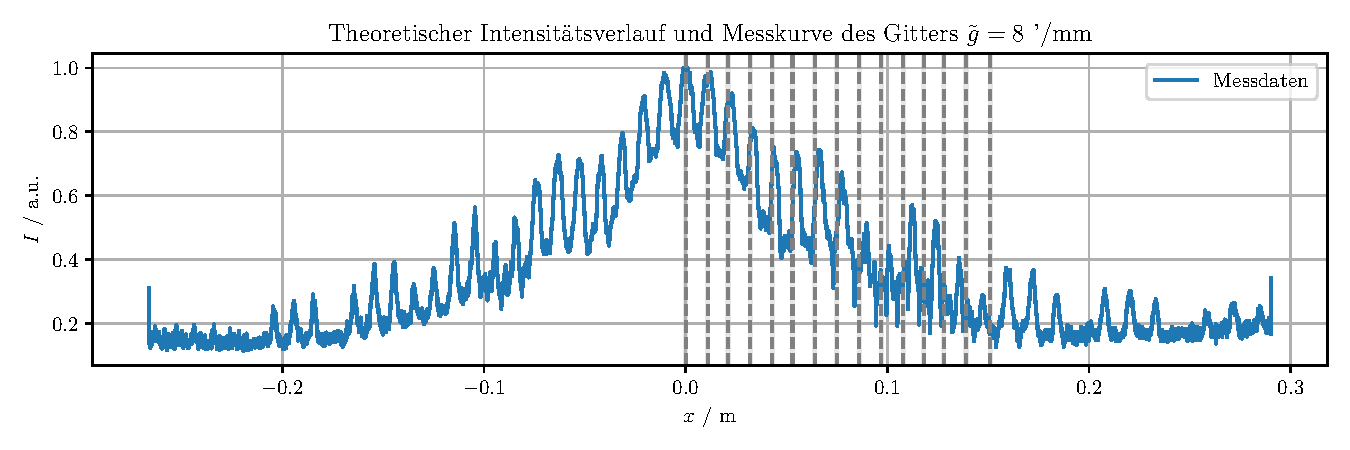
\includegraphics[width=\linewidth]{../python/plots/grating.pdf}
        \caption[Intensitätskurve Gitter]{Gemessener Intensitätsverlauf des Gitters, Messkurve aus \autoref{fig:DS_4_interferenzmuster} (rechts) extrahiert.}
        \label{fig:intensitaet_gitter}
    \end{samepage}
\end{figure}
%
Durch Äquivalenzumformung von \autoref{eq:intensity_gitter} kann schließlich die Gitterkonstante $g$ in \si{m} aus den gemessenen Positionen der Intensitätsmaxima aus \autoref{tab:messwerte_gitter} berechnet werden. Die resultierenden Werte werden wieder mit Hilfe einer Student-t-Verteilung statistisch gemittelt und korrigiert. Die Gitterkonstante ergibt sich zu:
\[g = \SI{96(9)}{\micro\meter}\]



\subsection{Shearing-Interferometer}
\label{subsec:auswertung_shearing}

Die in \autoref{tab:messergebnisse_shearing} tabellierten Größen werden zur statistischen Auswertung gemittelt und deren Standardabweichung mit einem Student-t-Korrekturfaktor mit Signifikanzniveau $1\sigma$ versehen. Daraus ergeben sich die folgenden Werte:
\begin{align*}
    l      & = \SI{9.8(3)}{\milli\meter} \\
    d      & = \SI{3.2(3)}{\milli\meter} \\
    \theta & = \SI{22(2)}{\degree}
\end{align*}
Für die Wellenlänge des Lasers wird der in \autoref{subsec:auswertung_doppelspalt} berechnete Wert herangezogen. Nun lässt sich der Radius $r$ der Wellenfront nach \autoref{eq:radius_wellenfront} berechnen und ergibt sich zu:
\[r=\SI{153(18)}{m}\]


\subsection{Polarisation}
\label{subsec:auswertung_polarisation}

Die am Lichtintensitätsmesser abgelesenen Intensitätswerte beider Messreihen werden pro Winkel statistisch gemittelt und mit einem Student-t-Korrekturfaktor versehen. Die so erhaltenen Werte werden inklusive ihrer Unsicherheiten (in Form eine halbdurchsichtigen Bands um den Graph) in \autoref{fig:auswertung_polarisation} dargestellt. Ebenfalls auf dieser Abbildung ist der theoretische Verlauf der Intensitätskurve gezeichnet, welche mit einem initialen $I_0 = \SI{1144}{lx}$ errechnet wurde.

\begin{figure}[H]
    \centering
    \begin{samepage}
        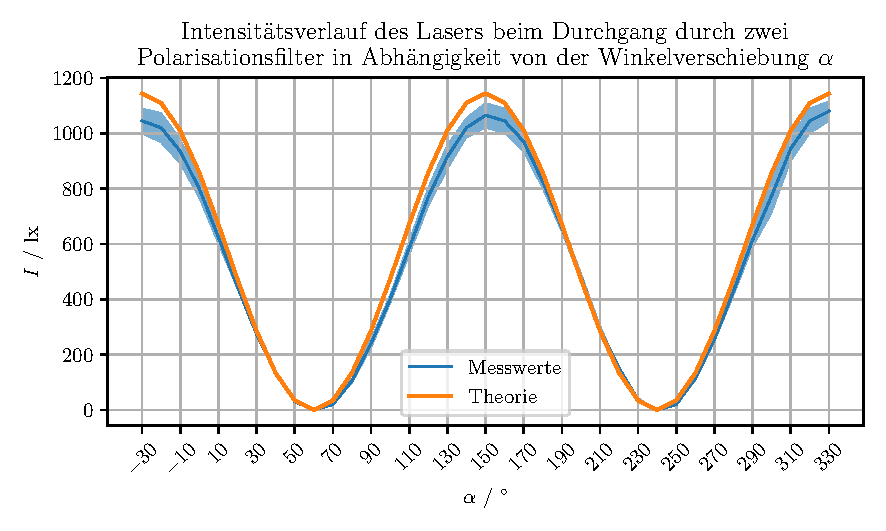
\includegraphics[width=\linewidth]{../python/plots/polarisation.pdf}
        \caption[Messkurve Polarisation]{Statistische Intensitätswerte am Lichtintensitätsmesser für die Messreihen des Laserdurchgangs durch zwei Polarisator. Die Messwerte sind mit einem Student-t-Korrekturfaktor versehen. Die Unsicherheit wird in Form des halbdurchsichtigen Bands dargestellt. Zusätzlich der errechnete theoretische Verlauf der Kurve.}
        \label{fig:auswertung_polarisation}
    \end{samepage}
\end{figure}


\subsection{Michelson-Interferometer}
\label{subsec:auswertung_michelson}

Mithilfe der Anzahl der generierten bzw. vernichteten Interferenzstreifen für sowohl Sammel- als auch Streulinse und der währenddessen notieren Weglängenunterschiedsänderung der Interferometerarme kann schließlich nach \autoref{eq:wegunterschied_anzahl} die Wellenlänge des Lasers berechnet werden. Diese ergibt sich sowohl aus den Messdaten der Sammellinse (Interferenzringe) als auch der Streulinse (Interferenzstreifen) zu:
\[\lambda_{\text{Sammellinse}} = \lambda_{\text{Sammellinse}} = \SI{530(30)}{nm}\]


\section{Diskussion}
\label{sec:diskussion}


\section{Zusammenfassung}
\label{sec:zusammenfassung}


\clearpage
% Literaturverzeichnis
\printbibliography

% Abbildungsverzeichnis
\listoffigures

% Tabellenverzeichnis
\listoftables


\end{document}